\documentclass{report}

\usepackage[utf8]{inputenc}

% cool tables
\usepackage{booktabs}
\newcommand{\ra}[1]{\renewcommand{\arraystretch}{#1}}

\usepackage{multirow}

\newcommand{\colorA}{\cellcolor{green!100}}
\newcommand{\colorB}{\cellcolor{green!60}}
\newcommand{\colorC}{\cellcolor{yellow!75}}
\newcommand{\colorD}{\cellcolor{orange!90}}
\newcommand{\colorE}{\cellcolor{red!80}}
% images
\usepackage{graphicx}
\usepackage{tabularx}
\usepackage{rotating}
\usepackage[table]{xcolor}
\usepackage{hyperref}
\usepackage{longtable}
% ?
\usepackage{float}



\usepackage[T1]{fontenc}
\usepackage{titlesec}
\usepackage{ltxtable}
% black square
\usepackage{amsmath}
\usepackage[parfill]{parskip}
\newcommand{\horrule}[1]{\rule{\linewidth}{#1}}


% referencing requirements
\newcommand{\refreq}[1]{\hyperref[req_#1]{#1}}
%numbers
%\renewcommand\thesection{\arabic{section}}
\pagenumbering{arabic} 

\title{
	\hrule
    \normalsize \textsc{Customer Driven Project}\\
    \Huge Rock Concert Audience as a Screen\\[10pt]
    \normalsize Project Report\\[10pt]
    Netlight AS
    \horrule{2pt}
    }  
\author{Agnethe Soraa,
Tomas Dohnalek,
Jan Bednarik,
Miloš Jovac \\
\normalsize Project supervisor: Anh Nguyen Duc}
\date{\today}

\definecolor{gray75}{gray}{0.75}
\newcommand{\hsp}{\hspace{20pt}}
\titleformat{\chapter}[hang]{\Huge\bfseries}{\thechapter\hsp\textcolor{gray75}{|}\hsp}{0pt}{\Huge\bfseries}

\begin{document}
\maketitle
\chapter*{Abstract}
The purpose of this document is to give an insight into the details of the planning, research, design and implementation of the task given in the course TDT4290 - Customer Driven Project. 
The project aims to give the students experience with a real project, and with a real customer. 
This gives the students an opportunity to combine both theory and practice. 
The customer for our project is Netlight AS.  

Our project will be about researching and implementing image processing. 
Naturally this means we also have to solve problems regarding mapping of mocked units to locations as a function of time. 
The environment takes place at a rock concert, which means we also have to solve issues with timing and syncing between multiple independent units.

This is a proof-of-concept task.  
All the research done will be documented, and used to argue for and against the solutions. 
We will also argue for and against alternative solutions. Everything from the planning to the complete conclusion is described in this report. 
To be able to solve these problems we have to start by investigating relevant technologies, and how we can make this possible.
The conclusion of this study allows us to create a system which showcases the real potential of our solution.


\chapter*{Preface}
This report is one of the deliverables in the course TDT4290 Customer Driven Project, which given by Department of Computer and Information Science at the The Norwegian University of Science and Technology, in the fall of 2013. Based on this project, the group?s work will be evaluated and graded by the appropriate personnel in charge of the course. 
We would like to thank our teaching supervisor, Anh Nguyen Duc , for regular input and guidance. 
We would also like to give a special thanks our customer, Peder  Kongelf from  Netlight consulting, who has given us the opportunity to work on such an interesting project, and also for being enthusiastic and helpful throughout the whole course.

\tableofcontents
\setcounter{page}{3}

\chapter{Introduction}
\section{General information}

The project is the making of the course TDT4290 Customer Driven Project. 
Customer driven project is a course held at The Norwegian University of Science and Technology, as mentioned briefly in the preface. 
This course accounts for 15 credits. 
It is a mandatory subject for the 4th year computer science students at IDI. 
The course aims to give the students a real experience with customers in a relevant IT-project. 
This course shall give the students a feel of managing a project in a group. 


All of the different groups is given one customer. 
The customer has put together a project, and to make sure the customer gets what he or she wants, there should be a close relationship with the customer.
Each group also receives an supervisor, which will support and give advice to the group. 


The delivery of the course is a report and a product, and this will be presented to an examiner. 
The report is the most important part of the project, and will contain all the documentation for this project. The course will provide realistic experience in both report writing and product development driven by a customer. 
This will help the students perform better when they are out in real life employment situations.

\section{Structure of report}
You can see the structure of this report in table \ref{tab:structure_of_report}.
\begin{table*}[!ht]\centering
\caption{List of all chapters and short description. }
\label{tab:structure_of_report}
\def\arraystretch{1.3}
\begin{tabularx}{\textwidth}{lX} \toprule[1mm]
\textbf{Chapter} & \textbf{Description} \\ \midrule
Chapter 1 & The introduction chapter introduces the problem, and introduces the members and stakeholders of this project.
This chapter also explains the motivation and goals. \\
Chapter 2 &  The preliminary Study chapter describes the work and research done. This chapter describes alternative solutions, and an evaluation these solutions. \\
Chapter 3 &  The planning chapter describes the project plan, the organization, quality assurance and planned workload.  \\

Chapter 4 &  The requirements chapter describes the requirements, both functional and non-functional. It also describes Use cases for the system. \\

Chapter 5 &  The test plan chapter contains the approach for testing with the overall test plan for the project.\\

Chapter 6	 &  The architecture chapter explains the structure of the system, and how it is put together. \\

Chapter 7	 &   The tools and strategy chapter describes the different tools we chose to use for this project.\\

Chapter 8-14 	&  In the sprint chapters the reader can see how the product has developed during the time of the project. This includes planning, architecture, the implementation, testing and evaluation of the sprint. \\

Chapter 15 	 &  The testing chapter describes the different tests. Everything from unit testing to acceptance testing. \\

Chapter 16 	 &  Evaluation chapter includes the team dynamics, risk evaluation, an evaluation of the customer, supervisor and of course the task. \\

Chapter 17 	 &  Conclusion chapter sums up the project, and discusses the solution, and looks at further work. \\

Chapter 18 	 &  The references chapter contains references. \\

Chapter 19 	 &  This chapter contains attachments. \\
\midrule
Appendix 	 &   The appendix contains user manual, installation guide, meeting minutes and more.\\

\bottomrule[1mm]
\end{tabularx}
\end{table*}

\section {Terminology}
\label{sec:terminology}
Since the customer is technically skilled and is used to use Scrum technology, we have adopted his terminology.
After few meetings with the supervisor it was settled that we must present our terminology to prevent from misunderstandings. 
There are also presented product related terminology that will be used in technical parts of this report.

\subsection{Scrum related terms}

\paragraph{User story}
is a short text of user's language of a system that describes user's interaction with the system.

User stories are actually narrative texts that describe an interaction of the user and the system, focusing on the value a user gains from the system.

\paragraph{Epic}
is a large \emph{user story} that will need to be broken down into smaller stories. It is too big to fit into a sprint, or it is unknown as to whether it is too big to fit into a sprint or not.

\paragraph{Task}
If user story is too complex, it can be divided into several tasks. 
Task is then basic unit of problem division.


\paragraph{Milestone}

\subsection{Product related terms}
\paragraph{Client user}
is a participant of concert who wants to actively take part in show and he can download client application.

\paragraph{Server user}
or simply \textbf{Manager} is a person who controls what media should be played on screen made from mobile phone's of users. 
He can also manage other general settings.

\paragraph{End user} is either manager or end client user.

\paragraph{Client} or \textbf{Client side} is an application controlled by client user and provides him opportunity to be part of the screen by displaying figures on his mobile.

\paragraph{Server} or \textbf{Server side} is and application controlled by manager and provides him opportunity to change the media displayed on screen.

\paragraph{Pixel} is a client user's mobile phone under control of manager.


\section{Project and project name}

The customer wants a product to make the audience as a screen on a rock concert. We decided to name the product "digital lighter". We agreed on this name because this product digitalizes the concept from "the old days", where the crowd at a concert held up lighters, to create a special atmosphere. 

\section{Project purpose and concept}

The audience members at a rock concert should be able to download a simple application to their cell phone, and register this through a simple GUI.
Behind the artist on stage there is a screen, with a simple camera on top. 
The camera is taking pictures of the audience. 
At special occasions the audience will be instructed, by the artist, to hold up their phones with the screen towards the stage. 
The mobile is a replacement for the lighter.  

On control a signal the application will fill the entire mobile screen with a single color.
The control signal can as an example say: " all pixels white". 
The signal will be specific for each application.
Each mobile will be a pixel in a larger picture, which will be presented on the big screen. 
What kind of picture the audience can create will depend on the number of people in the audience.   

As a motivation for the audience to hold up their phone, the camera on top of the screen will take pictures of the audience.
In that way the audience can see a reflection of them selves, and see what kind of picture they are creating together.

\section{Project goals}
Goals and objectives are statements that describe what the project will accomplish. The very first step in all projects: business, home, or education, is to define goals and objectives. 
This step defines the projects outcome and the steps required to achieve that outcome. 
It is important to spend sufficient time on this step, or else it can lead to unsuccessful project completion in many different ways. It can push the  a project intro overrun, territory battles, personality clashes, missed milestones, and unhappy customers. 
   
\label{sec:project-goals}

\subsection{Project goals}

\paragraph{Finish the project within the scheduled timetable}
Our goal is be to finished with the project within the given time frame. This means we must do everything possible to drive the project to the end and stay on time. Remember to avoid guessing in the planning of the scope.

\paragraph{Finish the project within the specified guidelines}
Another goal is to make sure we are meeting the customer's needs. We want "wow" the customer! 
This can be done simply by finishing the project with the specifics the customer really wanted. The best way to solidify this is to verify your accomplishment by customer hand off and close down.

\subsection{Group goals}
\paragraph{Receive a good grade}
Getting a good grade is important because it says something about what you have learned in this course. 
This is relevant in terms of what job we might get when we have graduated. It also shows an employer that we can work hard. 
\paragraph{Receive a good recommendation from customer/supervisor}
If we work really hard, and impress the supervisor and the customer it would be nice to get a recommendation. This would be a bonus for our CV.


\paragraph{Do the best we can with what we have been given}
There is no such thing as a perfect project.
Some projects run up against major odds and hurdles, and project goals were met because they did their best with what came their way. One of ours goals is of course to do the best with what we have been given.


\subsection{Personal goals}
\paragraph{Agnethe}

My personal goal is to learn about group dynamics and collaboration. Another goal is learn more about writing reports, because it is important to get some experience before writing the masters report. One of my goals is also to  satisfy our customer, and maybe get a good recommendation. It is also a great chance that I might work as an IT-consultant, and I want to learn as much as possible about this profession. I also  get better at holding presentations, because there will always be another presentation to hold. I also want to learn as much as possible about android and mobile development.

\paragraph{Jan}

This class was suggested to me by a few students who have already passed it. As from what I have learned it should be challenging and the students should receive a lo of experience while working on a project. From this point of view my personal goal is to improve my soft-skills regarding team collaboration as well as the technical skills, mostly the Java/Android programming. While I study at the Computer graphics department on my home university the image processing part of this project is also of the great value for me. I also expect to get the proper feedback from both the supervisor and the customer so I could learn from the mistakes or wrong approaches.

\paragraph{Milos}

is freerider.

\paragraph{Tomas}
I have chosen NTNU university for my exchange studies because of this class. 
I was expecting to improve my soft-skills, software engineering knowledge and also my written and spoken English and to be treated like in real project.
As this class has already started, I can add to my personal goals also learning Java programming language,
Android platform development and improving my skills concerning image processing.

\section{Stakeholders}

The stakeholders in this project is any person or organization, which has some interest or is affected by this project. Together they construct the different restrictions and goals for the project. 
You can see the organization chart in figure \ref{img:organization_chart}.

\begin{figure}[!ht]
    \begin{center}
    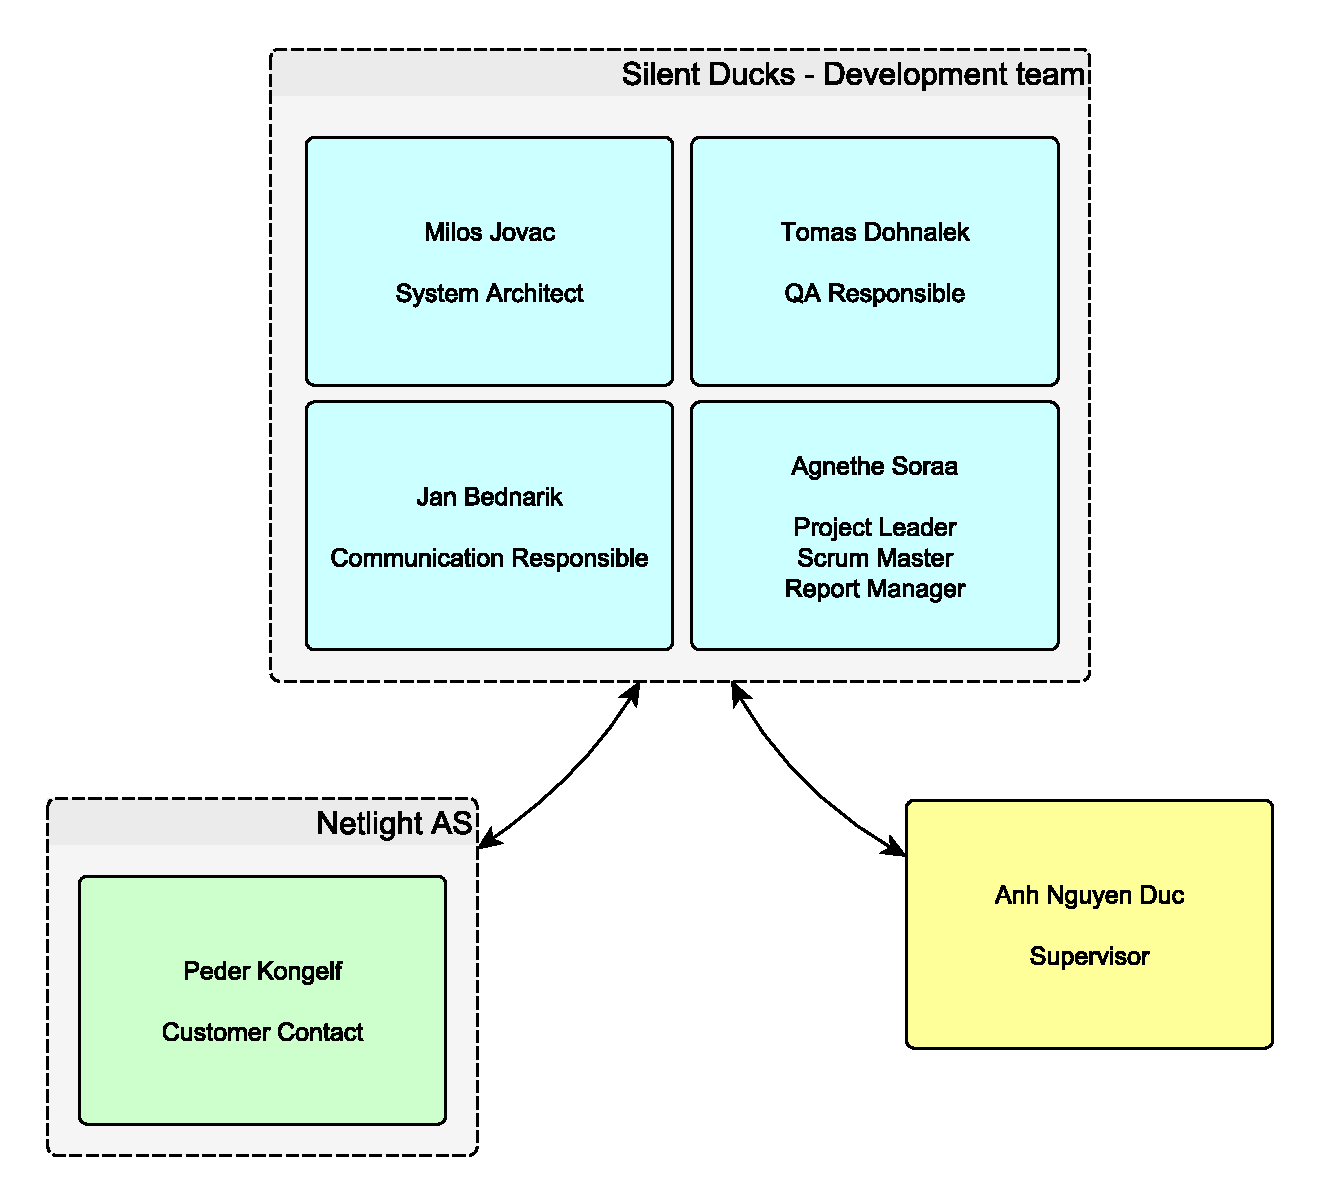
\includegraphics[width=12cm]{images/organization_chart.eps}
    \caption{Chart depicting team organization and its stakeholders.}
    \label{img:organization_chart}
    \end{center}
\end{figure}

\subsection{Customer}
Netlight AS is a consulting company engaged in IT and management. Their field of expertise is within IT management, IT governance, IT-strategy, IT-organization and IT-research. They deliver unique solutions based on their customers requirements. They operates throughout Europe with offices in Stockholm, Oslo, London, Munich and Helsinki. The company was founded at 1999 and employs to 500 employees. 
\subsubsection{Customer contact}
Peder Kongelf will be our contact person in Netlight. We will have weekly meetings with him to make sure the project is going in the right direction, and of course get opportunities to ask questions. This way we will get a better understanding of the project.

\subsection{Development team}
 The development team's role is, first of all, to meet all requirements presented by the customer and IDI. We are responsible for development of the project. We are also responsible for writing all the documentation for this course.  Our interest in the project is to receive experience with new technologies and project management, as well as to receive satisfactory grading. You can read about personal goals in section \ref{sec:project-goals}. 
 
 The project was intended for 5-7 students,but we are only 4 members in our team. This will, in some way, affect what the team can manage towards what was expected when the project was put together.

\subsection{Supervisor}

Anh Nguyen Doc is the supervisor assigned to this project from The Department of Computer and Information Science. The main responsibility of the team's supervisor is to overview the whole project and discuss the work done together with the future plans. Since the decisions and suggestions of this person are of the great importance the team agreed on holding the supervisor meetings once a week. The team should prepare the meeting minutes document and send it to the supervisor before the next meeting.


Of course the interest from the university in general is to provide some real experience to the students, and prepare them for the business world.


\subsection{End users}
Is a everyday person who uses the end product. Our plan is to release the product on the application store for Android. That way we can get feedback from someone other than supervisor and customer. 
\subsection{Stakeholder summary}
You can see the table with email contacts in table \ref{tab:stakeholders_summary}.

\begin{table*}[!ht]\centering
\caption{List of all stakeholders with their role and email contact. }
\label{tab:stakeholders_summary}
\def\arraystretch{1.15}
\begin{tabular}{lll}
\toprule[1mm]
\textbf{Person} & \textbf{Email} & \textbf{Role}\\
\midrule
Peder Kongelf & peder.kongelf@gmail.com  & Customer\\
\midrule
Anh Nguyen Doc	 & anhn@idi.ntnu.no & Supervisor \\
\midrule
Milos Jovac &  milosjovac@gmail.com & Team member  \\
Jan Bednarik &  ja.bedna1@gmail.com & Team member\\
Agnethe Soraa & agnethes0raa@gmail.com & Team member  \\
Tomas Dohnalek & dohnto@gmail.com & Team member \\
\bottomrule[1mm]

\end{tabular}
\end{table*}

\chapter{Preliminary studies}
This chapter is devoted to describing the outcomes of the preliminary research focusing on the similar already existing projects and technologies we could utilize.
In section \ref{txt:similar_projects} the similar projects will be described together with their relations to our project and their advantages and disadvantages. 
Then in the section \ref{txt:development technologies} the development technologies and collaboration tools will be presented with outcome of the overall research. 

%%%%%%%%%%%%%%%%%%%%%%%%%%%%%%%%%%%%%%%%%%%%%%%%%%%%%%%%%%%%%%%%%%%%%%%%%%%%%%%%%%%%%%%%%%%%%%%%%%%%
%%%%%%%%%%%%%%%%%%%%%%%%%%%%%%%%%%%%%%%%%%%%%%%%%%%%%%%%%%%%%%%%%%%%%%%%%%%%%%%%%%%%%%%%%%%%%%%%%%%%

\section{Similar projects} \label{txt:similar_projects}

We were not able to find any other service that would use exactly the same technical solution as compared to our product. 
Nevertheless a few similar entertainment services that aim to amuse the music concert audience already exist. 
These services basically encourage the audience to use either their smartphones or other device as the source of light that helps to create impressive and colorful show.

%==================================================================================================%

\subsection{Wham City Lights}

\subsubsection{Description}
The Wham City Lights is the mobile application developed by the one year old Baltimore based start-up \footnote{\url{http://whamcitylights.com/}}. 
As far as the Digital Lighter is concerned the Wham City Light service seems to be the closest solution as it works with the users' smartphones and uses them as a source of the light and even the sound.

Users attending the given concert only need to download and install the free application, start it and then hold their smartphones in the air.
The application then controls the color displayed on the smartphone screen, the camera flashes and the sound going out of the speakers and it creates the spatial soundscapes and lighting designs.
What is more the application do not require the Internet connection as the instructions are modulated into the ultrasonic inaudible signal that is being continuously transmitted during the performance.

Using this innovative technique all of the smartphones can be effectively synchronized so that the  changing lights and imagery on the phone follows and complete the music performance.
Nevertheless the so called light show must be pre-programmed and this system cannot determine the location of the mobile devices.

The demonstration of the real world performance of the application and the whole concept for that matter can be seen in the official Wham City Lights marketing video\footnote{\url{http://www.youtube.com/watch?v=faJ1Av5kBCE}}.

\begin{figure}[!ht]
	\centering
		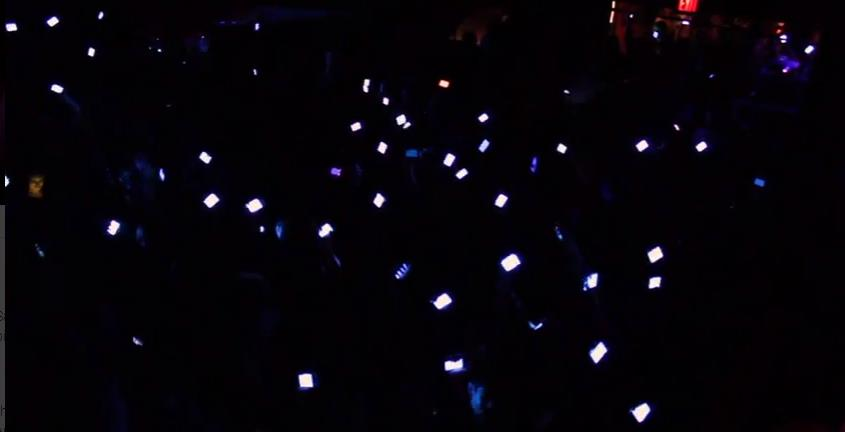
\includegraphics[width=10cm]{preliminaryStudies/wham_city_lights.jpg}
	\caption{Wham City Lights}
	\label{fig:wham_city_lights}
\end{figure}

\subsubsection{Impact}
The Wham City Lights application or its derivatives have been so far used on relatively many music events of the greater importance where several thousands of people were present and used the application. To list a few:
\begin{itemize}
\item America's Got Talent 2013
\item CMA Music Festival 2013
\item Intel sales conference 2013
\item Billboard Music Awards 2013
\item etc.
\end{itemize}

\subsubsection{Availability}
The application is available for the devices using Android or iOS operating systems and it can be downloaded from the Google Play\footnote{https://play.google.com/store/apps/details?id=com.whamcitylights} and App Store\footnote{https://itunes.apple.com/us/app/wham-city-lights/id580034697?mt=8} respectively. The developer nevertheless offers the customers the concert specific applications with relevant user interface built-in. As for the light show itself, programming part can be done either by the customer or the developer.

\subsubsection{Relation to our project}
Like our project the Wham City Lights application build upon users' smartphones that are remotely controlled in order to display intended imagery. 

\paragraph{Advantages}
The devices attending the light show do not need the Network connection and the displayed imagery is well synchronized with the music.

\paragraph{Disadvantages}
The location of the mobile devices cannot be determined and the different processing speed of the devices causes incorrect synchronization.


\subsection{Xylobands}

\subsubsection{Description}
So called Xyloband\footnote{http://xylobands.com/} is the invention of the company RB Concepts Limited. The device itself consists of the plastic bracelet that includes the LED diodes of the different colors and the microcontroller. 
The bracelets are controlled by the radio signal being broadcast from the stage and as a result they change their colors, flashes and in general create colorful imagery.

\begin{figure}[!t]
	\centering
		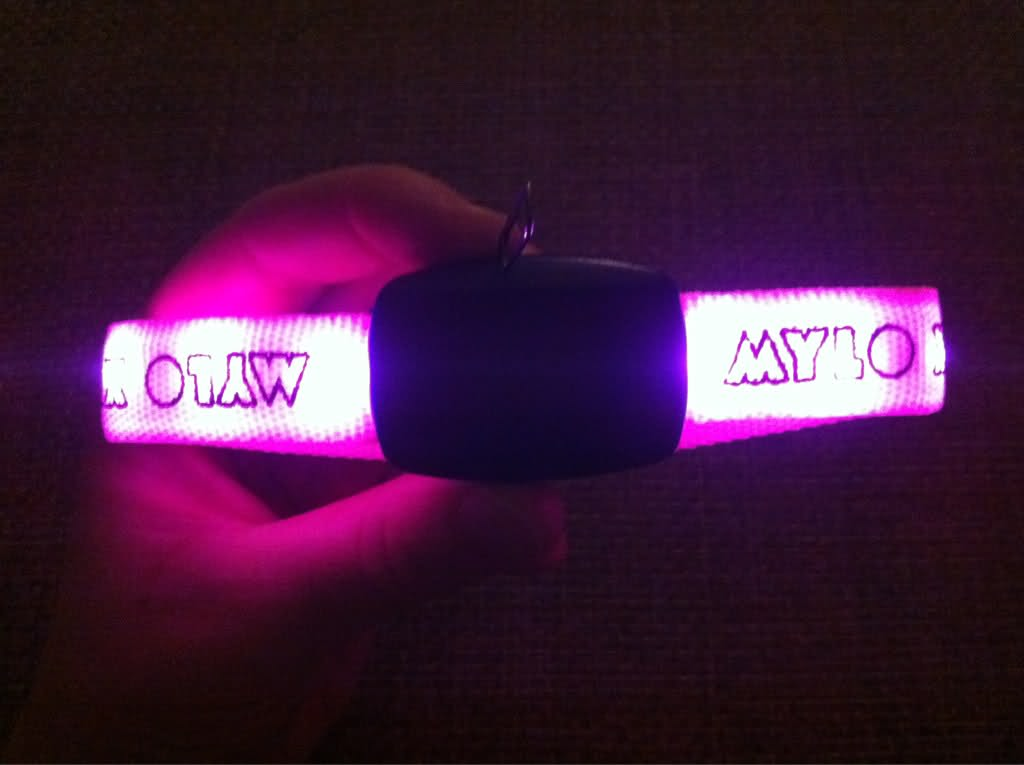
\includegraphics[width=10cm]{preliminaryStudies/xylo.jpg}
	\caption{Wham City Lights}
	\label{fig:xylo}
\end{figure}

\subsubsection{Impact}
Xylobands received great fame thanks to the well known British rock band ColdPlay which used them during their 2012 tour.

\subsubsection{Availability}
The bracelets can be ordered on the official Xylobands website.

\subsubsection{Relation to our project}
the Xylobands product is somewhat different from the Digital Lighter as it does not utilize the users' mobile devices. 
The similarity can be found in the way the bracelets are synchronized using wireless signal. 

\paragraph{Advantages}
The users do not need to bring their own mobile device and all of the audience have the possibility to become the part of the light show.

\paragraph{Disadvantages}
The location of the single participants cannot be determined.

%\section{Existing technologies and frameworks}
%\section{Evaluation of alternative solutions}

%%%%%%%%%%%%%%%%%%%%%%%%%%%%%%%%%%%%%%%%%%%%%%%%%%%%%%%%%%%%%%%%%%%%%%%%%%%%%%%%%%%%%%%%%%%%%%%%%%%%
%%%%%%%%%%%%%%%%%%%%%%%%%%%%%%%%%%%%%%%%%%%%%%%%%%%%%%%%%%%%%%%%%%%%%%%%%%%%%%%%%%%%%%%%%%%%%%%%%%%%

\section{Software development methodology}
A software development methodology is a framework used for structuring, planning and controlling the process of developing an information systems \cite{selectinMethodology}.
There will be presented a few of leading methodologies below. 

\subsection{Waterfall}
\subsection{Scrum}

After fast research and consultation with our mentor and customer(He has experience with CDP student group from last year), we decided to use SCRUM methodology for a few reasons. Requirements and scope of the undertaking were not that precisely defined at the time we had to decide on the methodology. Our approach therefore could not be founded on the sequential methodology as is "waterfall". We wanted to have frequent meetings with our customer and involve him in development process. Sprints in SCRUM allow us just that - 
to have meeting with customer at the end of every sprint, and plan next one together. Sprints does not have to be the same length so we can better managed developing process and risks, and we will be able to have as much sprints as possible under time limit of 13 weeks. SCRUM will give us derivatives that we can enhance in increments and allow us to gradually reduce the risk and keep our customer informed about our progress. SCRUM is also a very popular approach in the software industry, so it is a good choice to learn it.

\section{Development technologies} \label{txt:development technologies}

According to the customer's requirements the product must be executable on the mobile devices and it should utilize the image processing technologies as well. Therefore we had to make two main decisions - which mobile platform to prefer and which existing image processing libraries to use. Both of the decisions are explained in greater detail in sections \ref{txt:mobile_platform} and \ref{txt:image_processing_library}.

%==================================================================================================%

\subsection{Android} \label{txt:mobile_platform}

The mobile devices market is currently flooded with smartphones and tablets running on dozen of different platforms. 
But since we try to aim the application on as many users as possible the choice was relatively straightforward.
Considering the survey carried on by the well established analyst, the company IDC, as of Q2 2013 Google's Android OS held almost 80 \% of the market share\footnote{\url{http://www.idc.com/getdoc.jsp?containerId=prUS24257413}} leaving iOS, windows Phone, BlackBerry and others well behind.
What is more all of the members of our team posses the Android based smartphone thus we decided to choose the Android platform.

\subsubsection{Android SDK}

Google provides the Android developers with all the necessary tools and API's through the open source and free SDK\footnote{Software Development Kit}. While developing under SDK the Java programming language together with the Android event-driven architecture is used.

\subsubsection{Android NDK}

Through the NDK\footnote{Native Development Kit} Google provides the toolset allowing the programmers parts of the application using native-code languages such as C and C++.
We discussed using NDK just for the computationally demanding modules such as the image processing since the applications based on already compiled code tend to run faster.
Nevertheless we are allowed to scale the problem down and thus the use of Java perfectly suffices fr our purposes.
Should the customer require to scale the problem up we can switch to using NDK anytime.

%==================================================================================================%

\subsection{OpenCV} \label{txt:image_processing_library}

As far as the image processing is considered the outcome of our preliminary research is as follows.
Currently there exist a few open source and free libraries generally focusing on working with the multimedia.
OpenCV library is probably the most well-known library providing a broad range of image processing functions.
It is written and meant to be used in conjunction with C++ but the possibility to use Java already exists too.
The support for using OpenCV on Android platform is provided through the OpenCV4Android SDK that can be obtained from the official OpenCV website\footnote{\url{http://docs.opencv.org/}} and used for free.
So far we consider this toolkit to be sufficient for our needs but should we come across any problems we might be forced to switch to the combination of OpenCV, C++ and Android NDK.

%==================================================================================================%

\subsection{TestFlight}

TestFlight\footnote{\url{https://testflightapp.com/}} is a free web service for mobile developers that provides the tools to easily deploy and distribute the mobile application. What is more TestFlight offers the SDK for developers so that it can be integrated directly into the applications. The advantage of using the TestFlight is the fact that the developer is able to track the bugs, crashes and users' or testers' feedback. The customer suggested the team to use such a service and we had to choose between the TestFlight and similar service called HockeyApp. Unlike HockeyApp the TestFlight is a free service therefore we decided to adopt this service.

%%%%%%%%%%%%%%%%%%%%%%%%%%%%%%%%%%%%%%%%%%%%%%%%%%%%%%%%%%%%%%%%%%%%%%%%%%%%%%%%%%%%%%%%%%%%%%%%%%%%
%%%%%%%%%%%%%%%%%%%%%%%%%%%%%%%%%%%%%%%%%%%%%%%%%%%%%%%%%%%%%%%%%%%%%%%%%%%%%%%%%%%%%%%%%%%%%%%%%%%%

\section{Project management tools}
Since we use Scrum methodology, we were in need to find an appropriate management tool supporting Scrum. 
There exist many possible tools, but most of them are charged from
certain number of team members. 
Here are presented tools we have used for a testing purposes or in real development.

%==================================================================================================%

\subsection{Trello}
is a collaboration tool\footnote{\url{https://trello.com/}} that can organize tasks into various boards, it shows what task has been assigned to who and in what stage the task is.
Even though Trello supports a lot of features, it is not originally designed for Scrum use and there is no support of \emph{Epics}, \emph{Burn-down chart} and time tracking. Therefore after short discussion we have decided that Trello is not suitable for our purpose.

%==================================================================================================%

\subsection{Gravity} 
is a simple project management tool\footnote{\url{www.gravitydev.com}} currently in beta phase.
It supports splitting stories into tasks and also automatically calculates \emph{Burn-down chart}. 
Last but not least it supports it is free of charge for 5 team members, it supports issue tracking and support labels, which can be used for \emph{Epics}.
On the other hand it does not support time tracking.
You can see picture of Gravity's features in image \ref{img:gravity}. After a while it showed up that Gravity has some bugs since it is in Beta version and also it misses a time tracking feature.

\begin{figure}[!h]
	\centering
		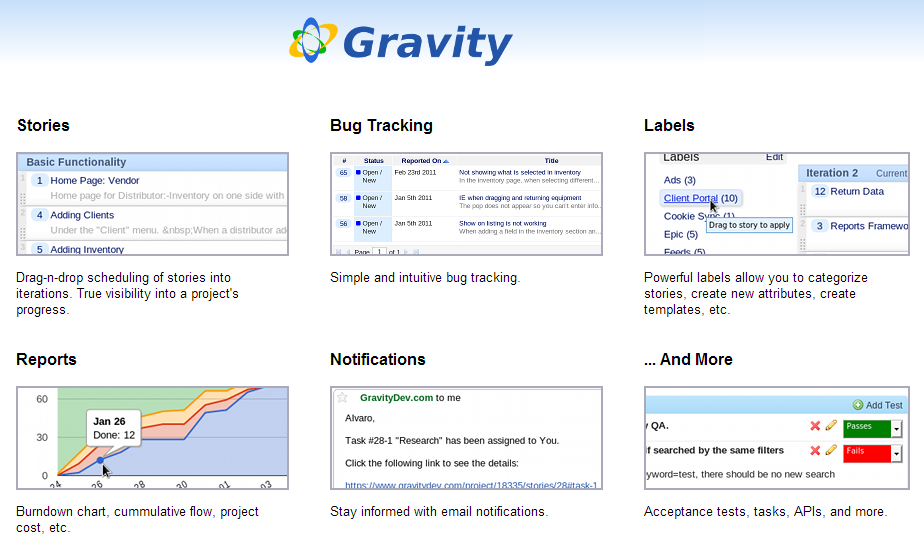
\includegraphics[width=11cm]{preliminaryStudies/gravity.png}
	\caption{Gravity features}
	\label{img:gravity}
\end{figure}
%==================================================================================================%

\subsection{Target Process} is a project management tool\footnote{\url{http://www.targetprocess.com/}} that supports different processes such as Scrum, Kanban and own process. 
To its main features belongs role distinguishing, different graphs (such as \emph{Burn-down chart}), time estimation and time tracking of both stories and its tasks, drag and drop prioritizing which makes it easy to use from customer side and different kinds of boards (diverse point of views on project).
On the contrary it also does not support Epics and it is much more complicated to use than other tools introduced.
You can see example of board in TargetProcess3 in image \ref{img:targetp}. Despite its complexity we decided to use the TargetProcess as it suited our needs the best.

\begin{figure}[!t]
	\centering
		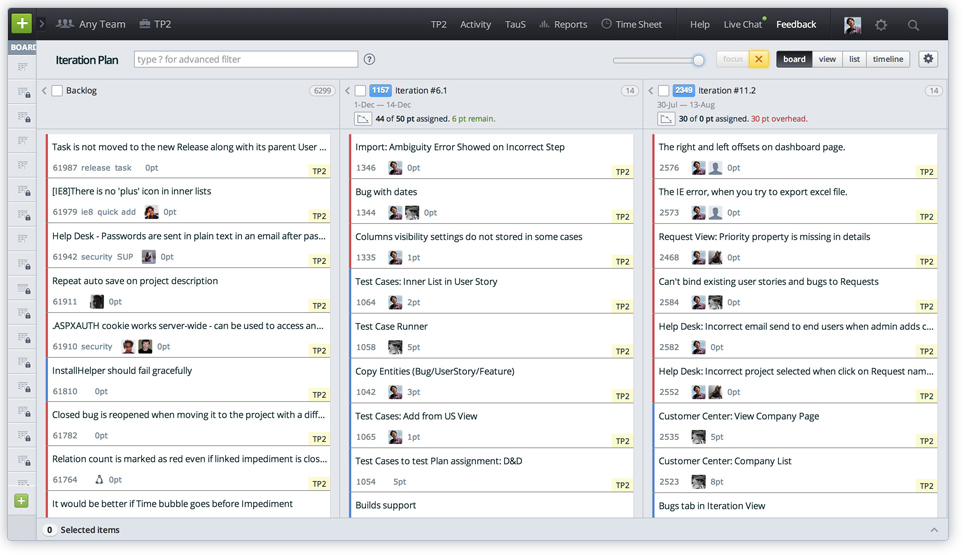
\includegraphics[width=11cm]{preliminaryStudies/targetp.png}
	\caption{TargetProcess's board}
	\label{img:targetp}
\end{figure}

%%%%%%%%%%%%%%%%%%%%%%%%%%%%%%%%%%%%%%%%%%%%%%%%%%%%%%%%%%%%%%%%%%%%%%%%%%%%%%%%%%%%%%%%%%%%%%%%%%%%
%%%%%%%%%%%%%%%%%%%%%%%%%%%%%%%%%%%%%%%%%%%%%%%%%%%%%%%%%%%%%%%%%%%%%%%%%%%%%%%%%%%%%%%%%%%%%%%%%%%%

\section{Version control tools}
Version control systems (VCS) are usually stand-alone applications but they can be integrated into other applications. These system usually allow users to browse previous versions of content. We have decided that we will use VCS both for source code of applications and for project report. 

As every member of the team had experience with different version control systems, they become our candidates. As our team works both on Microsoft Windows and GNU/Linux, it is necessary that chosen VCS supports clients in both platforms. Another criteria was support of online code repository free of charge.

%==================================================================================================%

\subsection{Subversion} or SVN is an open source centralized VCS and has many clients across different platforms. 
SVN is supported by Google Code\footnote{\url{http://code.google.com/}} repository.
SVN supports atomic commits, branching and more. Although this tool provides the user with all of the necessary functionality we decided not to use it as the customer suggested to use the other tool.

%==================================================================================================%

\subsection{Git} on the other hand is distributed VCS and offers immediate offline operations.
Projects like Linux kernel\footnote{\url{https://www.kernel.org/}} and Glibc\footnote{\url{https://www.gnu.org/software/libc/}} are using Git as a VCS.
Although Git was created by Linus Torvalds, there are Windows clients available.
Git is supported by GitHub\footnote{\url{https://github.com/}}, what is web-based hosting service for VCS. We have adopted Git as our version control system due to our customer suggestion, the distribution feature and our good experience with Github.
You can find our repository on \url{https://github.com/dohnto/CDP} page.

\begin{figure}[!t]
	\centering
		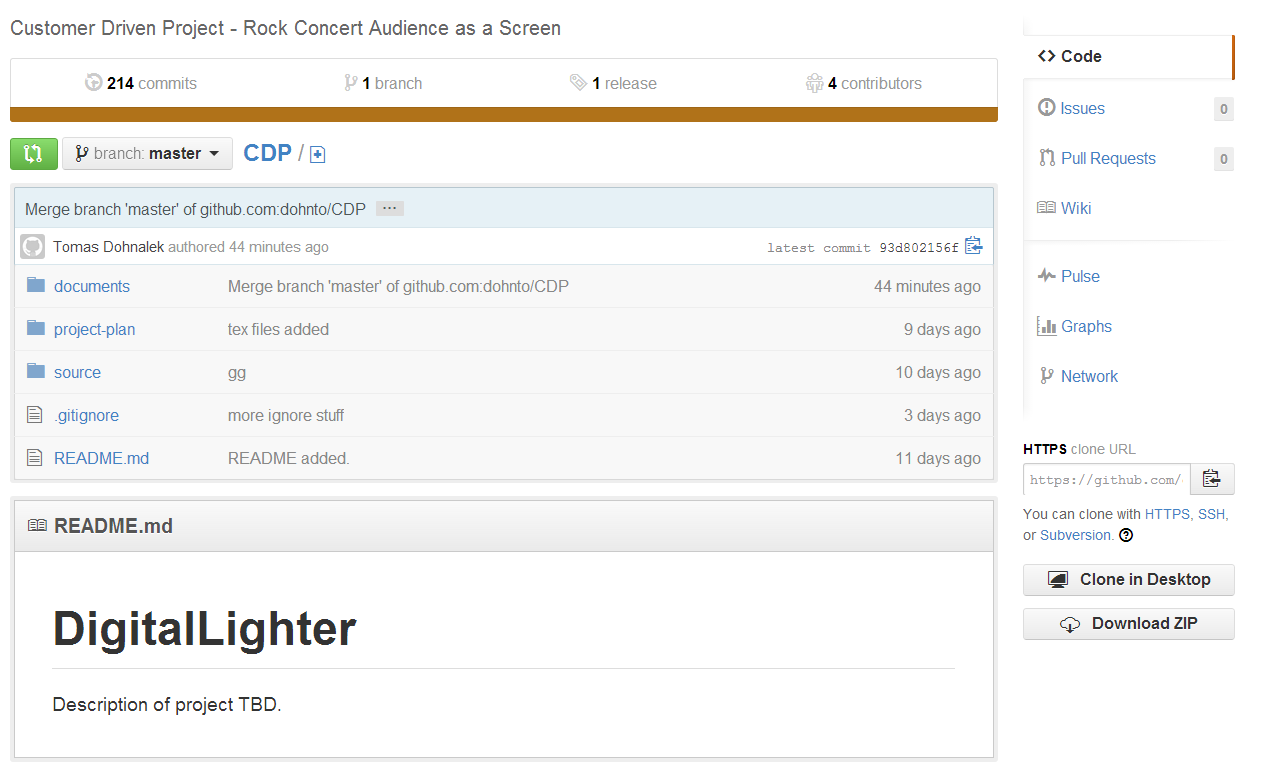
\includegraphics[width=10cm]{preliminaryStudies/git.png}
	\caption{Our github page}
	\label{img:git}
\end{figure}


%%%%%%%%%%%%%%%%%%%%%%%%%%%%%%%%%%%%%%%%%%%%%%%%%%%%%%%%%%%%%%%%%%%%%%%%%%%%%%%%%%%%%%%%%%%%%%%%%%%%
%%%%%%%%%%%%%%%%%%%%%%%%%%%%%%%%%%%%%%%%%%%%%%%%%%%%%%%%%%%%%%%%%%%%%%%%%%%%%%%%%%%%%%%%%%%%%%%%%%%%

\section{Communication tools} \label{txt:communication tools}
Regular Communication with stakeholders and creation of a positive understanding is one of the essential parts of the successful project that can help build effective long-term relationships all parties benefit from. Not only the development team should meet the customer and the supervisor on regular basis but there is also the need for easy distribution and sharing of all kind of the documents. As the time resources of all parties are limited the right collaboration tools enabling seamless and fast communication must be established.

There are certain standard tools that are widely used as a mean of exchanging both textual information and data files. The mainstream well known and effective tools include standard e-mail for messaging, tool for video conferencing, cloud system for data sharing and/or calendar for planning the meetings. Certain platforms providing all necessary tools exist, one can choose among solutions made by Microsoft, Apple, Google and Facebook to list a few most popular.

%==================================================================================================%

\subsection{Email}
Standard email messages will serve the purpose of the communication mean.

%==================================================================================================%

\subsection{Google Drive}
In order to provide the customer with the convenient overview of the work done all relevant documents including the meeting minutes, private notes taken during the meetings and the project report are stored on the Google drive cloud storage service and shared with the customer.

%==================================================================================================%

\subsection{Google Calendar}
The shared Google Calendar was established to keep track of arranged meetings.

%==================================================================================================%

\subsection{Skype}
The Skype is used as a videoconferencing tool as it is considered to be a software of a good quality and the customer disposes of the Skype account.

%==================================================================================================%

\subsection{Facebook group}
For the purpose of internal communication and data exchange among the team members a Facebook group was chosen.

%%%%%%%%%%%%%%%%%%%%%%%%%%%%%%%%%%%%%%%%%%%%%%%%%%%%%%%%%%%%%%%%%%%%%%%%%%%%%%%%%%%%%%%%%%%%%%%%%%%%
%%%%%%%%%%%%%%%%%%%%%%%%%%%%%%%%%%%%%%%%%%%%%%%%%%%%%%%%%%%%%%%%%%%%%%%%%%%%%%%%%%%%%%%%%%%%%%%%%%%%

\section{Documentation tools} \label{txt:documentation tools}

There are basically two options for documentation writing. It is either possible to use WYSIWYG editor such as Microsoft Word, Libre Office or document preparation system based on markup language such as \LaTeX.

\subsection{LaTeX}

It was strongly suggested by the customer to use the latter one as the reports written using \LaTeX  tend to make more professional impression.




\chapter{Planning}
In this chapter we are planning the project in general. It is hard to come up with a detailed plan for each sprint now, but this is a rough plan for the whole project. After doing a preliminary study we have made some decisions about methodology tools, technology, collaboration, and a rough project plan. Planning increases the efficiency and it reduces the risks involved. It also facilitates proper coordination within a development team, and this will help us maintain a good control. Planning will help us to achieve our goals by using the available time and resources, and of course planning helps in decision making  

\section{Methodology choice - Scrum}
After fast research and consultation with our mentor and customer(He have experience with CDP student group from last year), we decided to use SCRUM methodology for a few reasons. Requirements and scope of the undertaking were not that precisely defined at the time we had to decide on the methodology. Our approach therefore could not be founded on the sequential methodology as is "waterfall". We wanted to have frequent meetings with our customer and involve him in development process. Sprints in SCRUM allow us just that - 
to have meeting with customer at the end of every sprint, and plan next one together. Sprints does not have to be the same length so we can better managed developing process and risks, and we will be able to have as much sprints as possible under time limit of 13 weeks. SCRUM will give us derivatives that we can enhance in increments and allow us to gradually reduce the risk and keep our customer informed about our progress. SCRUM is also a very popular approach in the software industry, so it is a good choice to learn it.

\section{Organization}
\begin{table*}\centering \ra{1.3}
    \caption{Skills and previous experience table. Coding:
        \textcolor{green!100}{$\bullet$} expert,
        \textcolor{green!60}{$\bullet$} experienced,
        \textcolor{yellow!75}{$\bullet$} neutral,
        \textcolor{orange!90}{$\bullet$} little experience,
        \textcolor{red!80}{$\bullet$} no experience}
    \label{tab:skills}
    \vspace{2mm}
    \begin{tabular}{lcccc}
    \toprule
                                & Agnethe   & Tomas & Milos & Jan \\
    \midrule
    \textbf{Leadership                 } & \colorB & \colorE & \colorD & \colorC \\ 
    \textbf{Scrum                      } & \colorB & \colorE & \colorE & \colorE \\ 
    \textbf{Mobile software development} & \colorC & \colorE & \colorB & \colorE \\ 
    \textbf{\LaTeX                     } & \colorE & \colorB & \colorE & \colorB \\ 
    \textbf{Network programming        } & \colorD & \colorC & \colorC & \colorC \\ 
    \textbf{Image processing           } & \colorE & \colorC & \colorE & \colorD \\ 
    \textbf{Java                       } & \colorC & \colorD & \colorA & \colorE \\ 
    \textbf{C++                        } & \colorE & \colorB & \colorC & \colorB \\ 
    \textbf{Testing                    } & \colorE & \colorB & \colorD & \colorC \\
    \bottomrule
    \end{tabular}
\end{table*}

\subsection{Role Assignment}
To assign roles according to our skills and previous experience we have decided to make a survey of relevant knowledge. 
Results of this survey can be seen in table \ref{tab:skills}. 
This table was used as a base for our role assignment.
In the beginning, during planning, we did not establish so many roles, but during the development process itself we found out that some of them are necessary. 
Nevertheless we use only few roles and the responsibility of unused roles (mention in compendium) are distributed to all members. 
We decided to embrace this as a development team were we are all equal.
The assigned roles can be seen in table \ref{tab:roles}. 

\begin{table*}\centering \ra{1.3}
    \caption{Assigned roles and their responsibilities}
    \label{tab:roles}
    \vspace{2mm}
    \begin{tabularx}{\textwidth}{llX}
    \toprule
    Role    & Person   & Responsibility \\
    \midrule
    \textbf{Project Leader}             & Agnethe &
        Responsible for progress of the project according to the plan.
        Distributes work to group members.
        Has final call in arguments.\\
    \textbf{System Architect}             & Milos &
        Check consistency and analyze all layers of the product. \\
    \textbf{Scrum Master}             & Agnethe &
        Leads the scrum stand-ups. \\
    \textbf{Communication Responsible}  & Jan &
        Responsible for communicating with customer and supervisor.
        Regularly send meeting minutes, agenda and other documents to customer and supervisor. \\ 
    \textbf{QA Responsible} & Tomas &
        Ensure a quality of all documents and end-product.        \\ 
    \textbf{Documentation Responsible} & Agnethe &
        Responsible for delegating and supervising work on final report.        \\         
    \bottomrule
    \end{tabularx}
\end{table*}

\section{Risk Management}
In the table \ref{tab:risks} the consequence and possibility in a number between 1-10. The risk, or the riskfactor, is the consequence multiplied with the possibility. The risks in this table is very obvious ones. 

Other risks we can see from analyzing the skill table. If for example the only two persons on the team who are familiar with image processing is away, then this will be a risk. There is a great possibility that this kind of task will take longer time then planned for. 

Also if some of the rows in the skill table all were painted red, which would imply that the team had experience with this, then this would be a risk. In such a case, we would have to talk to our customer and consider scaling down this task. 
\ref{tab:risks}

\begin{sidewaystable}
    \caption{Handling risks}
    \label{tab:risks}
    
    \centering \ra{1.3}
    \vspace{2mm} %\rotatebox{90}{
    \begin{tabularx}{500pt}{XcccXX}
    \toprule
        Event & Consequence & Possibility & Risk  & Reactive Measures & Proactive Measures \\
    \midrule
Someone gets sick & 4     & 5     & 20    & Other people do more work.  & Free weekends \\
Coding problems & 4     & 7     & 28    & Talk to supervisor \& Guru office & preparing for the task \\
Testing problems & 4     & 4     & 16    & Talk to customer about reformulating requirements & Double check requirements with customer \\
Implementing things we are not supposed to & 7     & 6     & 42    & Try to adopt functionality or start all over & Don't do anything that is not in backlog and keep good communication with customer \\
Dead end with technologies & 8     & 8     & 64    & Talk to supervisor \& Guru office & Do thoroughly research \\
Unrealistic time estimate & 7     & 8     & 56    & Work overtime  & Planing poker \\
Frequent changes in requirements specification & 6     & 3     & 18    & Renegotiate with a customer & Try no to change finished modules and keep weekly meetings with the customer \\
Customer too ambitious & 9     & 5     & 45    & Renegotiate with a customer & Keep customer informed about what  to expect \\
Hardware problems & 9     & 3     & 27    & Obtain a new one & Keep your devices updated \\
\bottomrule
\end{tabularx}
\end{sidewaystable}
\subsection{Limitations}
\label{sec:limitations}
We are developing this project under a few technical, resource, time and knowledge limitations. 

Our biggest limitation is the image processing part. Half of the team has no experience with this, and the other half has little experience. Their experience is mostly theoretical information about the subject, and practical experience is preferred. We are aware of this limitation, and our plan is to learn by doing. We are going to start developing, and teach ourself while coding. We chose this approach because we do not want to spend more time than necessary doing research.

Another limitation is lack of experience with Mobile development within the development team. All of the team members have Android phones, and to be able to test our application, we have to develop an Android application. Only one team member have experience with this. 

If we are not scaling down the project, then we do not have all necessary resources to test the system. As an example we do not have a huge audience. Also  we do not have access to a big screen etc. This is also a limitation.  

As this course last for a 13 weeks, it is normal that we have to make some trade-offs.
This project is technically difficult, and there is a limited amount of time. 


\section{Communication}
Specific guidelines and practices were adopted
so that the team and the customer could continuously verify that the project development keeps the right direction and that the requirements are being fulfilled.

\subsection{Customer collaboration}
Since the scope of the project and the actual requirements are determined by the customer it is essential to establish tight collaboration practices and even involve the customer in the collaboration tools the team uses. In the next paragraph the main means utilized for interaction with the customer are listed. 

\paragraph{Meetings}
We agreed on holding the weekly meetings taking approximately 60 minutes. The standard agenda consists of the approval of the meeting minutes summarizing the last meeting, comments on the meeting minutes and the specific issues regarding the team-customer collaboration and technical issues. As the customer is located in Oslo the meetings will be carried out using the video-conference devices provided by the NTNU (accessible in the Accenture Lab) and Skype software. Contents of each meeting including the topics discussed, decisions made and the future plans are summarized in the meeting minutes. The team should provide the customer with the meeting minutes document before the next meeting is held.

\paragraph{Email}
Standard email messages will also serve the purpose of the communication mean, both team and the customer agreed on responding to the queries as soon as possible.

\paragraph{Documents}
In order to provide the customer with the convenient overview of the work done all relevant documents including the meeting minutes, private notes taken during the meetings and the project report are stored on the Google drive cloud storage service and shared with the customer.

\paragraph{Other tools}
As mentioned earlier the team decided to utilize the Target Process 3 as a collaboration tool suitable for handling Scrum-driven projects. The customer was invited to join the framework so that he could observe the development process more closely. Thanks to the software tool the customer is able to easily adjust the order of the user stories according to his preferences.

\subsection{Team collaboration}
Mostly during the pre-study phase the developers need to distribute and maintain the information considered important for the next work. The Facebook group was chosen and set up to serve this purpose as it disposes of the tools suitable for exchanging website links, opinions and multimedia.

It has been also decided that the project report should be written continuously by all members as a part of our daily workflow. Through this practice the team will be able to keep track of the amount of work done and all members will make sure they understand well what direction the project is aiming.

\section{Duration and workload}
 Compendium proposed week workload 25 person-hours per week. During our internal meeting we have decided that each member will spend 30 hours per week because our team consists only of 4 members. We agreed on fixed daily working hours so that we could distribute the workload through the whole semester. We will do daily stand-ups according to Scrum methodology.

\section{Project scope}
After third meeting with our customer we decided to lay out the scope of the project that is tangible and doable under 13 weeks. Customer idea although good and innovative has one flaw - it is a huge undertaking!

As we operate under certain limitations we explained in \ref{sec:limitations}, we agreed with customer on next terms:
\begin{itemize}
	\item Take project title as domain of work and not final product.
	\item Scale down problem but attack all main problems of the domain.
	\item When designing architecture disregard scaling of product.
	\item Disregard some of problems that are not important for final prototype, but  with approval of a customer before making this kind of decision.
\end{itemize}

\section{Project plan}
\subsection{General plan for all of the sprints}

In general the sprints will last for two weeks. The only sprints that does not have that length, is the first and the last. This is because these two are more related to getting started, and finishing the project. The other sprints will have a more general approach. 

After each sprint we have a sprint review with the customer. The sprint reviews takes place every other Thursday, which means that the Wednesday before, the team has to prepare for the review. In each sprint review we both present and demonstrate what we have done so far. After the presentation we are doing a retrospective with the customer. It is important to evaluate our sprint delivery the customer. After the retrospective we will plan the next sprint, and now the customer can prioritize which user stories he wants us to work on next. The Friday after the sprint review, the team will do a detailed planning of the next sprint. 

On the Thursdays in between we have weekly meetings with the customer. It is important to have good communication with the customer. These meetings gives us opportunities to ask questions, and to make sure that we are on the right track.

You can see detailed sprint decomposition in figure \ref{img:sprint_detail}.

\begin{figure}[!h]
    \begin{center}
    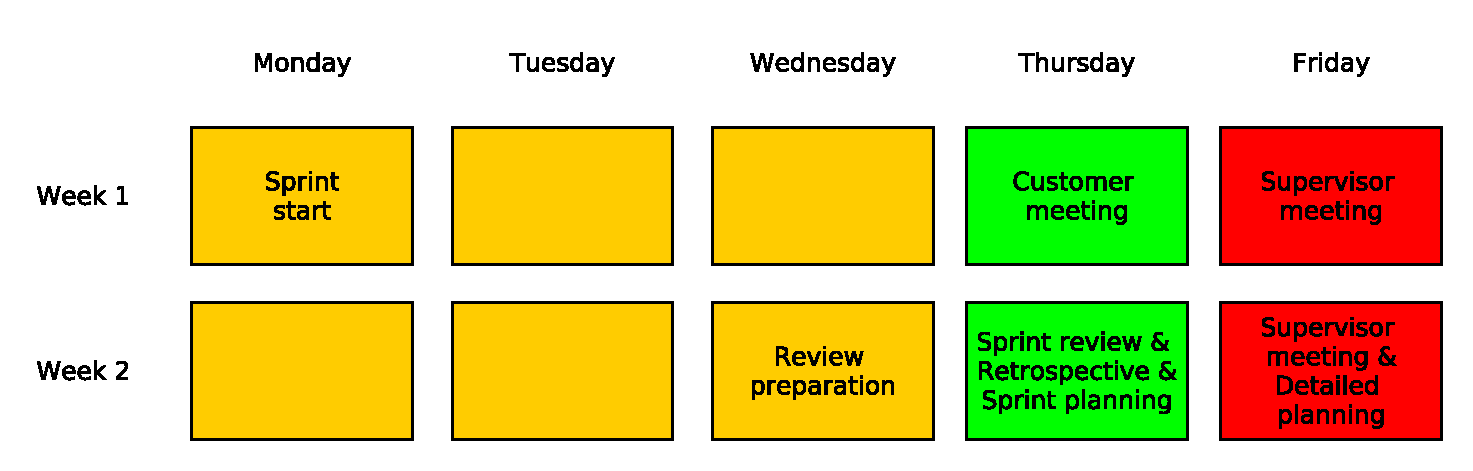
\includegraphics[scale=0.4]{images/sprint_detail.pdf}
    \caption{Diagram depicting detailed sprint decomposition.}
    \label{img:sprint_detail}
    \end{center}
\end{figure}

\subsection{Phases}
\subsubsection{Sprint 0}
We have embraced Sprint 0 as a preliminary sprint, when we can set up all necessary collaboration tools, equipment, prepare templates for meetings and mainly to acquaint ourselves with Scrum methodology. The original plan was to finish sprint 0 on 8th of September, but we have decided to terminate it prematurely due to finishing sprint goals in shorter time than we had expected. Other reason for terminating the sprint was desire to start actually working on the product itself.

\paragraph{Sprint duration:} from 22nd of August until 1th of September
\paragraph{Sprint goals:}
\begin{itemize}
    \item Read compendium
    \item Find and agree suitable collaboration tools
    \item Start working the Project plan
    \item Fill backlog with stories
    \item Assign roles to members of the team
    \item Assign a name to our project
\end{itemize}

\subsection{Milestones}

\subsubsection{Product Milestones}

We set milestones in order to more accurately ascertain whether or not the project is on schedule. After finishing some group of the milestones we will have running prototypes (Deliverables). There are 4 prototypes in total we 
agreed on. After reaching point of 4 prototypes we will have meeting with our customer about how the project is about to continue. The 3th prototype implies that all milestones are reached. 
Although the order of prototypes may look like a waterfall approach that is not the case.
Overview of all milestones and 4 prototypes (Deliverables).

\paragraph{Obedient client  - Prototype 1}
\begin{itemize}
	\item Put "Hello World" project to gitHub and pull it to every group member's local storage.
	\item Set up protocol for client \& server.
	\item Make server able to listen for clients.
	\item One client connects to the server.
	\item The server sends command to one client.
	\item The client receives one command.
	\item The client "plays" one command (white light 10 seconds).
\end{itemize}

\paragraph{Obedient crowd - Prototype 2}
\begin{itemize}
	\item Multiple clients connect to the server.
	\item The server sends same signal to multiple clients.
	\item The server sends multiple different commands to the client.
	\item The client plays commands (Red light 2 seconds, Green light 2 seconds).
\end{itemize}

\paragraph{Traffic light control - Prototype 3}
\begin{itemize}
	\item Server identifies one client from light.
	\item Server maps one client to grid (4 quads).
\end{itemize}

\paragraph{Digital lighter stone age - Prototype 4}
\begin{itemize}
	\item Server identifies multiple clients from light.
	\item Server maps all devices to the grid.
	\item Server play whole picture to the grid.
\end{itemize}


\begin{itemize}
	\item Finish of Project Plan document.
	\item Learn about team dynamics.
\end{itemize}

\section{Gantt diagram}
You can see the Gantt chart in figure \ref{fig:gantt}.
\begin{figure}
    \begin{center}
        \label{fig:gantt}
        \caption{Gantt Chart: Allocation of sprints into weeks.}
        \begin{sideways}
            \begin{gantt}{9}{14}
                \begin{ganttitle}
                   \titleelement{Week}{14}
                \end{ganttitle}
                \begin{ganttitle}
                   \titleelement{1}{1}
                   \titleelement{2}{1}
                   \titleelement{3}{1}
                   \titleelement{4}{1}
                   \titleelement{5}{1}
                   \titleelement{6}{1}
                   \titleelement{7}{1}
                   \titleelement{8}{1}
                   \titleelement{9}{1}
                   \titleelement{10}{1}
                   \titleelement{11}{1}
                   \titleelement{12}{1}
                   \titleelement{13}{1}
                   \titleelement{14}{1}
                \end{ganttitle}
                \ganttbar{Sprint 0}{0.5}{1.5}
                \ganttbarcon{Sprint 1}{2}{2}
                \ganttbarcon{Sprint 2}{4}{2}
                \ganttbarcon{Sprint 3}{6}{2}
                \ganttbarcon{Sprint 4}{8}{2}
                \ganttbarcon{Sprint 5}{10}{2}
                \ganttbarcon{Sprint 6}{12}{1.5}
            \end{gantt}
        \end{sideways}
    \end{center}
\end{figure}


\section{Quality Assurance}

\section{Measurement of Project Successes \#supervisor}
To measure success of our end-product we have to set up some criteria to be fulfilled. The product should pass all test-cases and function according to customer's requirements.

\subsection{Description ?}
\subsection{Result schedule ?}


\chapter{Requirements}
In this chapter expected behavior of product and its resulting requirements will be described. 
First there will be introduced simple life cycle of the product.
Although project title was accepted as a domain and not a final product, following requirements could be applied also on project that is not scaled down.

\section{Description}
To clarify and properly explain life cycle of one run of server side application, its usage and possible requirements, structure of UML's activity diagram was adopted. 
Therefore we show in figure \ref{img:activity_diagram} interaction between manager and one client user.
Notice that there are some actions of both Manager and client user which do require direct manipulation with mobile phone or other actors such as "Notice users to raise their mobiles", "Raise mobile", "Put down mobile" and more.

\begin{figure}[h!]
    
    \begin{center}
    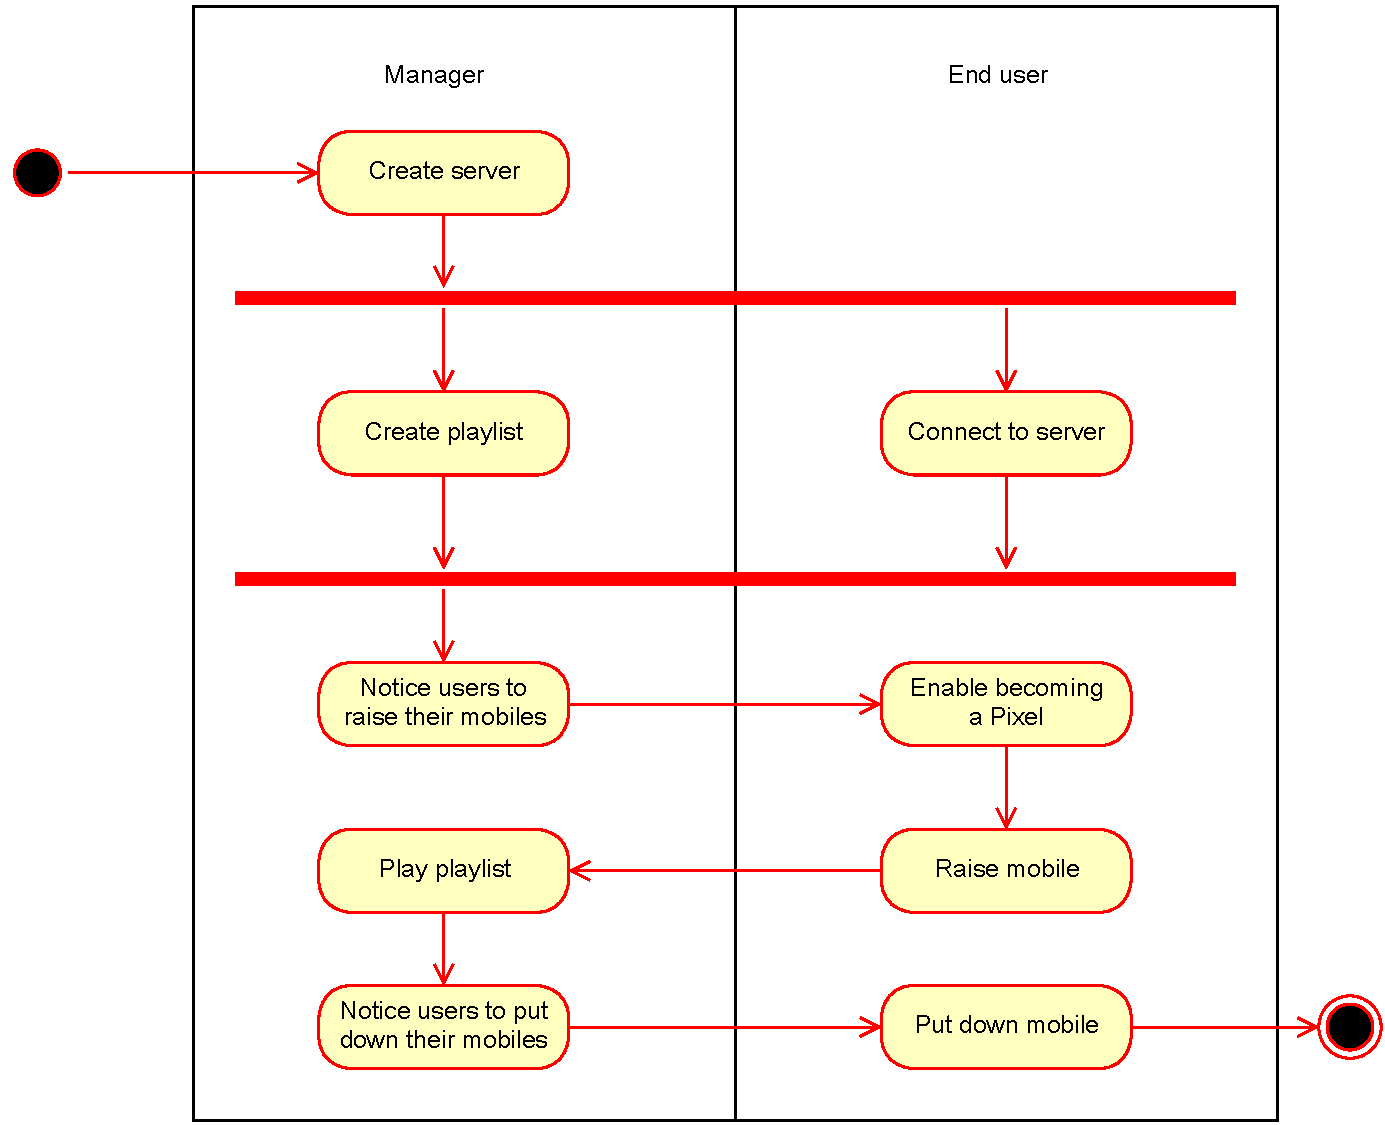
\includegraphics[scale=0.4]{images/activity_diagram.pdf}
    \label{img:activity_diagram}
    \caption{Activity diagram depicting basic scenario of using product with all actors.}
    \end{center}
\end{figure}


\section{Use case diagram}
As we have defined terminology in section \ref{sec:terminology} we will use actor's names according to that terminology.
In the figure bellow use case diagram \ref{img:usecase} of the whole system  is shown.

\begin{figure}[h!]
    \begin{center}
    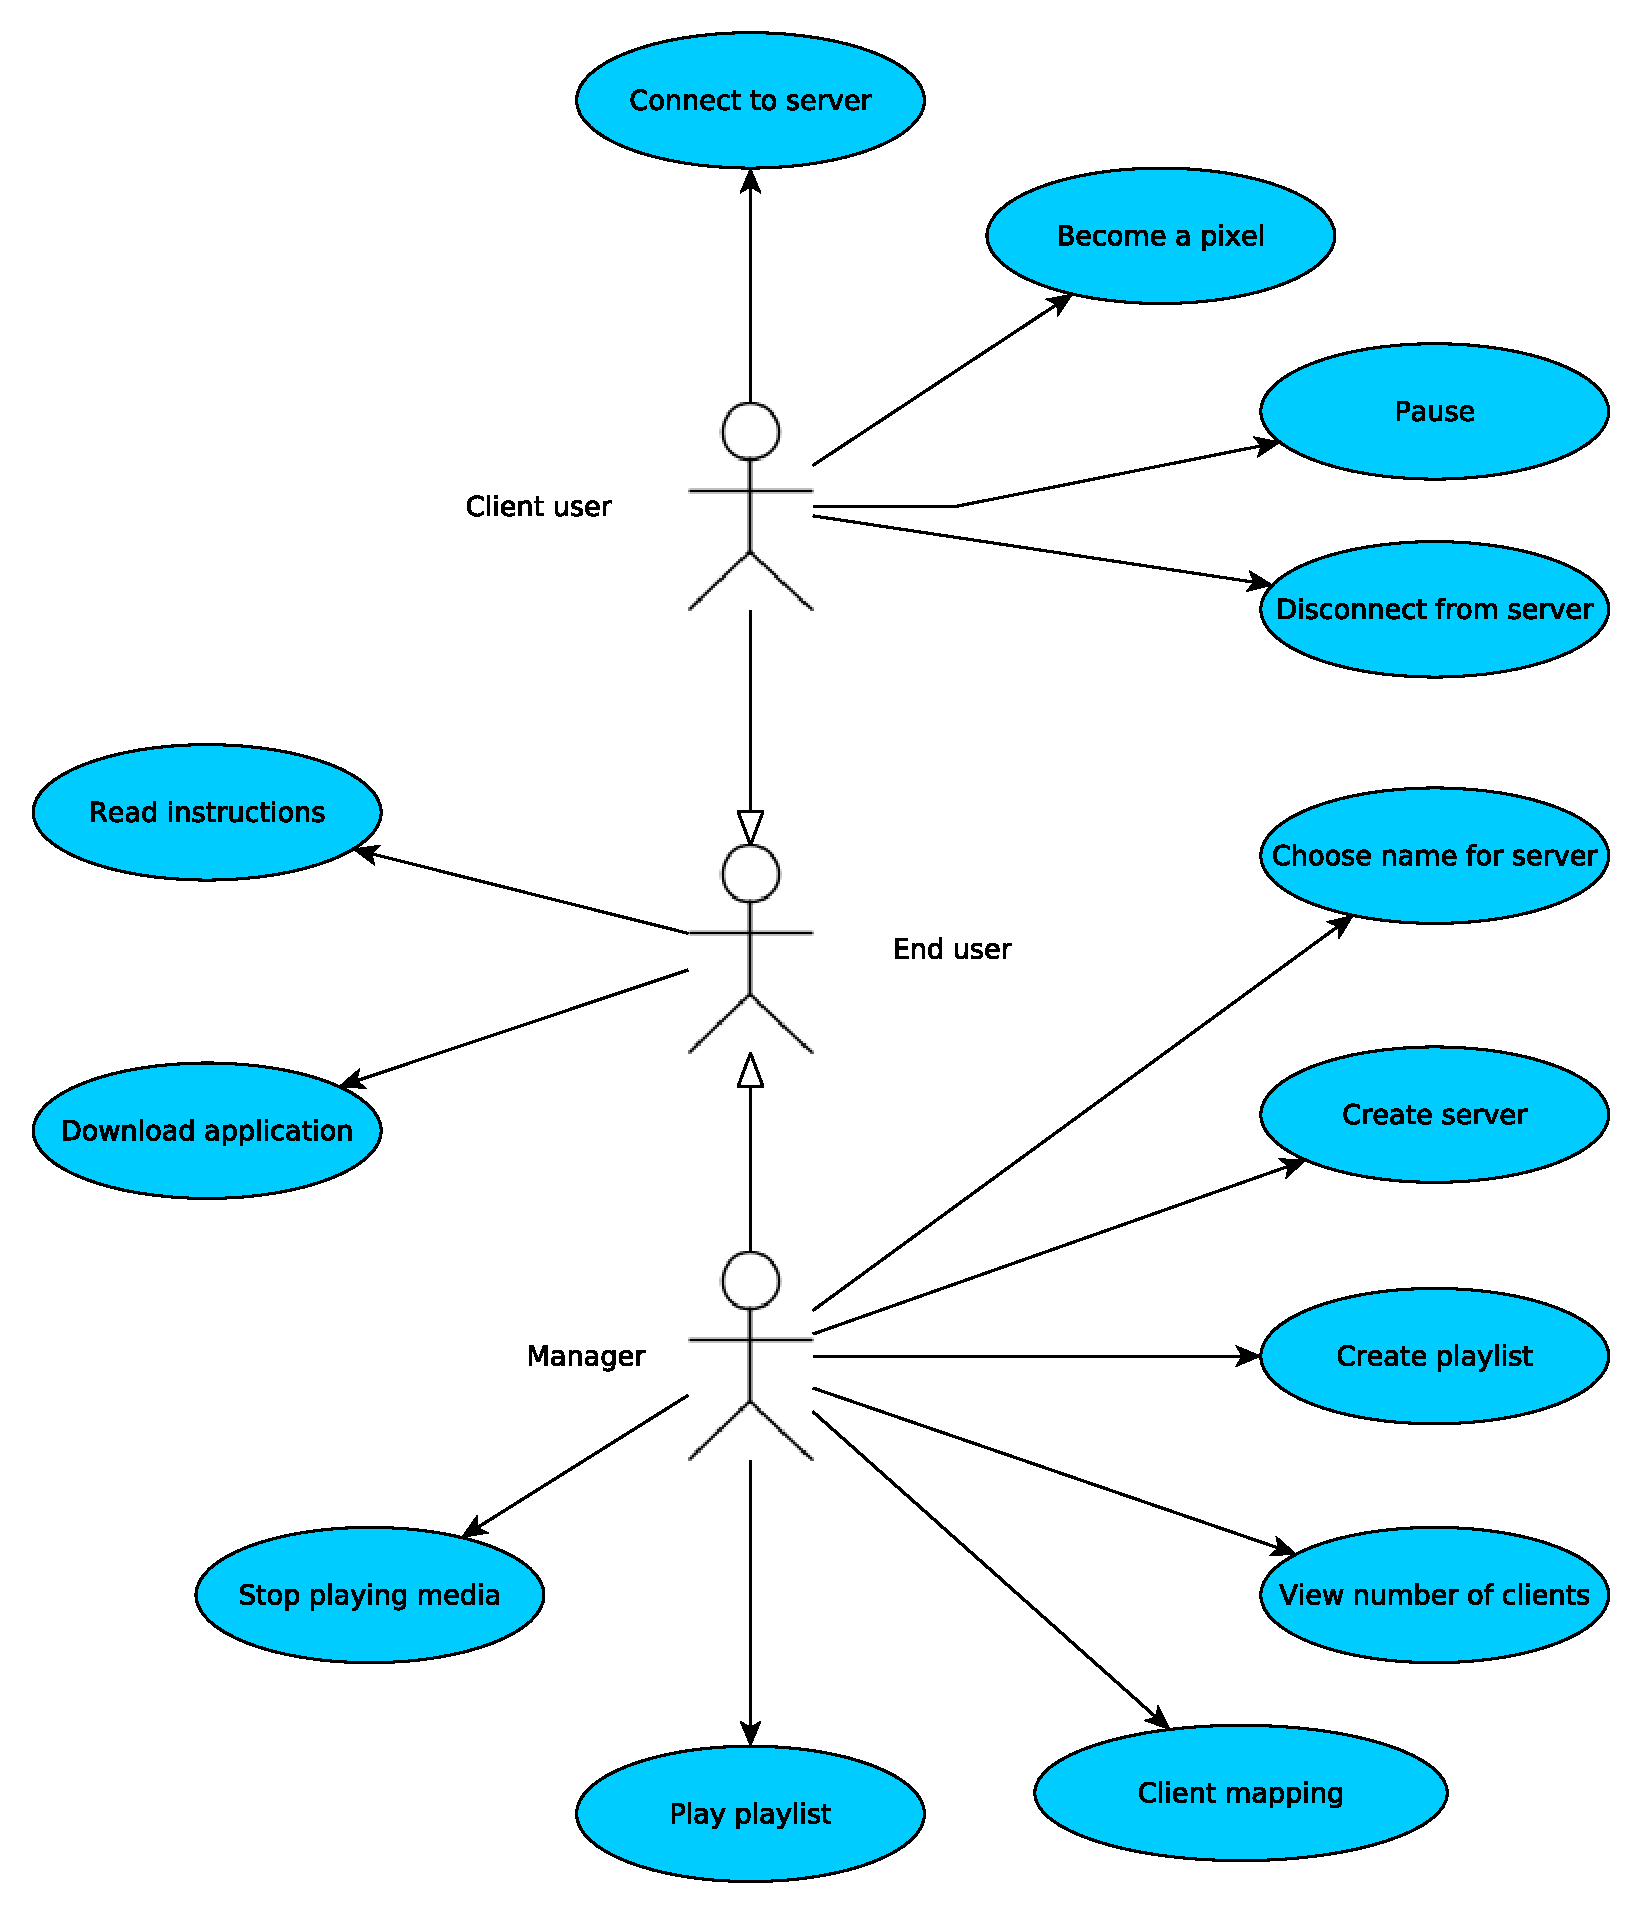
\includegraphics[scale=0.4]{images/usecase.pdf}
    \caption{Use case diagram depicting all actors.}
    \label{img:usecase}
    \end{center}
\end{figure}

\section{Requirements}
Requirements can be divided into two categories - functional and non-functional. 
Functional ones describe what should product do, its specific behavior or function.
On the other hand non-functional requirements cover what product is.


\subsection{Functional}
According to use case diagram \ref{img:usecase}, functional requirements were created.
You can see list of those requirements from end user's point of view below.

\begin{enumerate}
	\item[\textbf{E1}] \label{req_E1}
		I as a end user want to be able to read instructions.
	\item[\textbf{E2}] \label{req_E2}
		I as a end user want to be able to download relevant application from mobile application store.
\end{enumerate}

You can see list of functional requirements from client user's point of view below.
\begin{enumerate}
	\item[\textbf{C1}] \label{req_C1}
		I as a client user I want to easily choose to which server/concert stage I would like to connect.
	\item[\textbf{C2}] \label{req_C2}
		I as a client user I want to connect to chosen server.
	\item[\textbf{C3}] \label{req_C3}
		I as a client user I want to become a \emph{Pixel}.
	\item[\textbf{C4}] \label{req_C4}
		I as a client user I want to be able to pause being a Pixel.
	\item[\textbf{C5}] \label{req_C5}
		I as a client user I want to be able to disconnect from server/stage.
\end{enumerate}


You can see list of functional requirements from manager's point of view below.
\begin{enumerate}
	\item[\textbf{M1}] \label{req_M1}
		I as a manager I want to be able to choose name for my server/stage.
	\item[\textbf{M2}] \label{req_M2}
		I as a manager I want to be able to create a server.
	\item[\textbf{M3}] \label{req_M3}
		I as a manager I want to be able view attendance.
	\item[\textbf{M4}] \label{req_M4}
		I as a manager I want to be able to start mobile phone localization.
	\item[\textbf{M5}] \label{req_M5}
		I as a manager I want to be able to choose playlist to be played.
	\item[\textbf{M6}] \label{req_M6}
		I as a manager I want to be able to start playing given media.
	\item[\textbf{M7}] \label{req_M7}
		I as a manager I want to be able to start pause playing the media.
	\item[\textbf{M8}] \label{req_M8}
		I as a manager I want to be able to start pause stop the media.
\end{enumerate}

\subsubsection{Detailed use cases}
In this section there will be described some use cases in detail.
\begin{table*}[!h]
	\def\arraystretch{1.25}
	\caption{Use case detail: Create playlist}
	\label{tab:usecase1}
	
	\begin{tabular}{p{\textwidth}}
		\toprule
		\textbf{Use case detail: Create playlist} \\
		\midrule
		Actors: Manager \\
		Conditions:
		\begin{enumerate}
			\item Manager had created server.
		\end{enumerate}
		Events flow:
		\begin{enumerate}
			\item Use case starts when manager choose option "Create playlist".
			\item Application will display list of possible media (videos, images) that can be played.
			\item Manager can preview specific media (view on his own screen).
			\item Manager chooses media to be played, order of choosing will be order of playing.
			\item Manager confirms the playlist.
			\item Use case ends.
		\end{enumerate}
		Alternative flow:
		\begin{enumerate}
			\item Manager can quit the screen and return to main menu anytime.
		\end{enumerate}
%		\\ 
		\vspace{0.6em}
		\hrule
%		\\[0.1pt]
%		\bottomrule[1mm]
	\end{tabular}
\end{table*}

\subsection{Non-functional}
You can see non-functional requirements listed below.

\begin{enumerate}
\item[\textbf{N1}] \label{req_N1} Product must work as a server and client architecture.
\item[\textbf{N2}] \label{req_N2} Client side application must work on at least one mobile platform.
\item[\textbf{N3}] \label{req_N3} Application must be deployed to relevant mobile application store.
\item[\textbf{N4}] \label{req_N4} The product must be scalable - it must work with different count of mobile phones.
\item[\textbf{N5}] \label{req_N5} The product must be prepared for future using outside of rock concert domain.
\item[\textbf{N6}] \label{req_N6} Final product must be finished until 21st of November 2013 and presented to the committee and the customer.
\end{enumerate}

\subsubsection{Quality attributes}
\phantomsection
\label{sec:quality_attributes}

\paragraph{Accessibility}
is the degree to which a the product is available to as many people as possible. 
Accessibility can be viewed as the "ability to access" and benefit from the product. 
To achieve this we plan to release the product on the Android Play Store, and we are also using TestFlight to make the applications as accessible as we can.

\paragraph{Interoperability}
describes the extent to which systems and devices can exchange data, and interpret that shared data. Digital Lighter server and client application should be able to mutually share specific structure or format of data that is preserved and unalterd during the process.  

\paragraph{Maintainability}
is the ease with which a product can be maintained. This means the product needs to isolate defects or their cause, prevent unexpected breakdowns, correct defects and repair or replace faulty components. If one component need to be replaced, then the system should do this without having to replace still-working parts. The product also needs make future maintenance easy.

\paragraph{Modifiability}
is all about handling changes, and this is including the extent to which this modification affects other functions. 
Code must be prepared for changes, and this can only be done by increase cohesion, and reduce coupling. 
If the modules get built smaller, the risk of having to make a change will be reduced. 
Team should also make sure that dependencies are restricted. 
Increasing the cohesion, or interdependency within modules, can affect build time, load time, initialization time or run time, therefore some trade-offs have to be done.

\paragraph{Performance}
is about managing system resources in the face of particular types of demands to achieve acceptable timing behavior. 
Performance can be measured in terms of throughput and latency. 
Performance can be improved by reducing demand, or by managing resources more appropriately. 
Reducing demands will have the side effect of reducing fidelity, or refuse service to some requests. 
Managing the resources more fitting can be done through scheduling, relication, or simply increase the resources available.

WRITE MORE HERE WEHN WE KNOW MORE!!


\paragraph{Usability}
Usability is the ease of use and learnability of the product.
Usability includes methods of measuring usability, such as analysis of needs or the study of the principles behind an object's perceived efficiency or elegance. We want our product to be easy to use, understandable, and easy to learn.  

\section{Summary}
In this chapter was explained how the application's basic life-cycle looks like and there was introduced Use case diagram \ref{img:usecase}.
According to Use case diagram \ref{img:usecase} there were created \emph{Epics} which serve as a requirements. 
After that non-functional requirements were introduced.
In following chapters each user story which is connected to relevant requirement will be referenced with requirement's identification.

As you could see, client user's interaction with both applications is rather simple (and as our customer suggested the user interface is not core of the work) the main attention will be focused on image processing, network programming and mapping devices into screen.

\begin{figure}[!ht]
    \begin{center}
    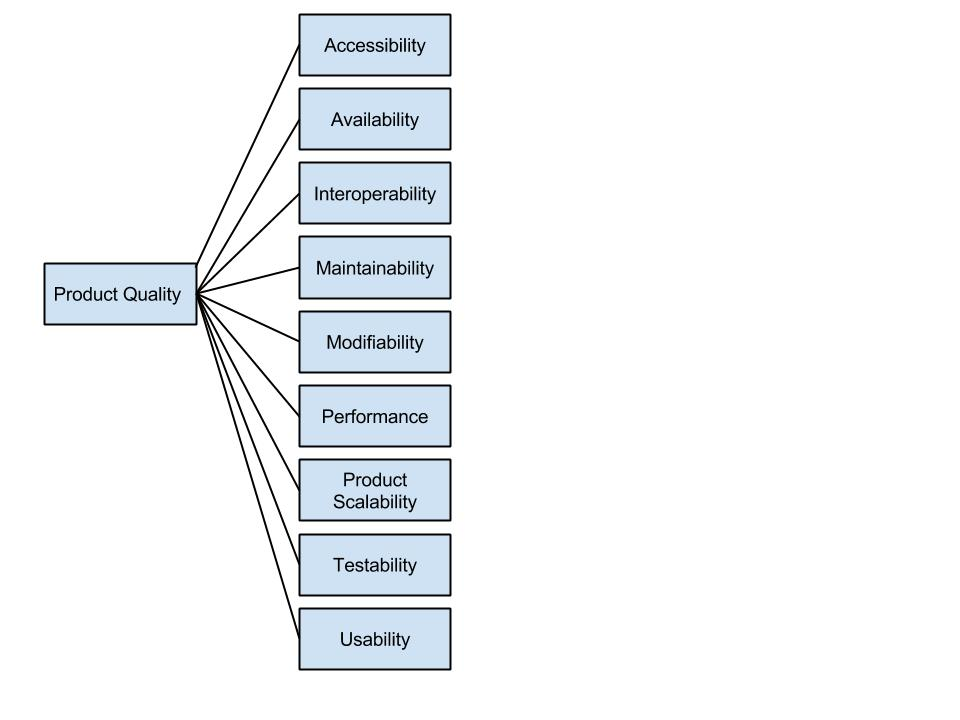
\includegraphics[scale=0.4]{images/qualityAttributes.jpg}
    \caption{Quality attributes.}
    \label{img:qualityAttributes}
    \end{center}
\end{figure}

%\chapter{Test plan}
%\section{Approach}
\section{Templates}
\section{Responsibilities}
\section{Test criteria}





\chapter{Software Architecture}
In this chapter, product architecture is described using 4 + 1 architectural view model.
It is based on the multiple concurrent views and therefore better explanation of architecture can be provided.

\section{4 + 1 view model}
\subsection{Logical view}
The description of the functional requirements of the architecture. The client and the server are decomposed into a set of key abstractions, taken(mostly) from the problem domain, in the form of objects or object classes.
\subsection{Development view}
\subsection{Process view}
\subsection{Physical view}
\subsection{Scenarios}
Use case diagrams can be considered as scenarios, therefore introduced diagram \ref{img:usecase} in Requirements chapter can be considered as a scenario.

\section{Used design patterns}
\subsection{Strategy}
\subsection{Model-View-Controller}
\subsection{Observer}

\chapter{Sprint 0}
In this chapter Sprint 0 will be described. It is written about what the team did during the first sprint, which also was a planning period for the team. At the end there will be evaluation of the  whole sprint, and answers to following questions: What went well? What could be improved? 

\section{Sprint planning}
The Sprint 0 is embraced as a preliminary sprint, where team can set up all necessary collaboration tools, equipment, prepare templates for meetings and mainly to acquaint team members with Scrum methodology. The original plan was to finish sprint 0 on 8th of September, but it have been decided to terminate it prematurely due to finishing sprint goals in shorter time than expected. Other reason for terminating the sprint was desire to start actual work on the product itself.

The user stories are listed in Table \ref{tab:sprint0stories}. Since software collaboration tool was used when sprint was already in progress, team did not manage to estimate the time needed to complete each story beforehand and thus the column \textbf{Est.} is left empty.

%\begin{longtable}{cX|cc}
%\textbf{ID} & \textbf{Description} & \textbf{Hours estim.} & \textbf{Hours spent} \\
%259 & \LaTeX template for minutes project plan & 5 & 4 \\
%259 & \LaTeX template for minutes project plan & 5 & 4 \\
%\end{longtable}

%\caption{User stories selected for Sprint 4.}
  \label{tab:sprint4stories}
 \def\arraystretch{1.25}
 
\begin{longtable}{ccXcc}

\toprule[0.5mm]
\multirow{2}{*}{\textbf{ID}} &
\multirow{2}{*}{\textbf{Ref.}} & \multirow{2}{*}{\textbf{Description}} & \multicolumn{2}{c}{\textbf{Hours}} \\
 					& & & \textbf{Est.} & \textbf{Sp.} \\
%\textbf{ID} 	& \textbf{Description} 	& \textbf{Est.} & \textbf{Sp.} \\
\midrule
\textbf{I4.1} 	& 	& {\bf As a server I need to link the devices' location with their ids.}	 &  52	& \textbf{48} \\

\textbf{I4.2} 	& 	& {\bf As a server I need to identifiy multiple clients from light.}		 &  19	& \textbf{18} \\

\textbf{I4.3} 	& 	& {\bf As a server I need to map all available devices to grid.} 			 & 22 & \textbf{18} \\	

\textbf{I4.4} 	& 	& {\bf As a server I need to play the whole media to the grid.} 			 & 37 & \textbf{34} \\
	
\midrule
		
				&& \textbf{SUM:}		&		130	& \textbf{136}
 \\																			
\bottomrule[0.5mm]
\end{longtable}


\section{Sprint goals}
\begin{itemize}
    \item Read compendium
    \item Find and agree suitable collaboration tools
    \item Start working on the Project plan
    \item Fill backlog with stories
    \item Assign roles to members of the team
    \item Assign a name to our project
\end{itemize}


\section{Testing}

Only the third party products were tested during the sprint 0. Team focused on testing the online team collaboration tools including Trello, described in Section \ref{subsec:TrelloToolDescription}, Gravity, described in Section \ref{subsec:GravityToolDescription} and TargetProcess, described in Section \ref{subsec:targetProcessToolDescription}. The outcomes of our research are described in Section \ref{sec:management_tools}.

\section{Occurring risks}

One of the major risks team came across were the limitations of the selected collaboration tools used for controlling the Scrum process. As team members were learning all the perks of using the Scrum methodology it was continuously discovered that neither Trello nor Gravity software tools suited team's needs and more time searching for another tool and setting it up again had to be spent. A few difficulties regarding the version control system Git prevents merging individual versions of the project plan document. This is considered as an risk so team spent significant amount of time solving these issues.

\section{Customer feedback}

The outcomes of preliminary studies have been presented to the customer. The customer was also walked through the collaboration tools and provided with the access to all of the team's resources so that the team and the customer would be able to collaborate more tightly. The customer was satisfied with the amount of the work done and approved the TargetProcess to become the team's main collaboration tool. Since the team managed to finish all of the selected user stories the customer agreed with the accelerated end of Sprint 0.

\section{Retrospective}
Since each complex software project requires that the team would go through the certain initiative tasks such as the assignment of the team roles, agreeing on the meetings, setting up the communication and collaboration tools etc., the Sprint 0 cannot be really thought of as a fully-fledged sprint. Team mainly focused on pre-studying the scrum methodology, communicating with the customer and the supervisor, clarifying the requirements and researching both the collaboration and development tools.

The working was started immediately after the first meeting with the customer was held. Besides the time spent on setting the tools we mainly focused on writing the project plan as this is a project where the amount of documentation is expected to be extensive. 

In order to reflect on the past sprint and to learn from the mistakes done it is necessary to answer two essential questions: "What went well" and "What could be improved".

\subsection{What went well}
Three online collaboration tools (Trello, Gravity and TargetProcess) were evaluated so that the suitable one could be find. The initiation tasks were finished earlier than expected and the Sprint 1 could be started earlier. All of the members' computers were set so that all of the tools would work. The team also got familiar with the concept of user stories, assigned a few of them to Sprint 0 and managed to finish all of them. All of the members were committed to spend the same amount of working hours.

\subsection{What could be improved}
During the first days the team was not operating efficiently due to the fact that team started to write the project plan without any clear specification of the document structure. Once the structure was agreed on the team members were able to work on the single tasks efficiently again without any need for unnecessary communication overhead and negotiations. Lack of experience in using the Scrum process resulted in imprecise usage of the user stories concept. The team should carry out additional research regarding the Scrum process in order to follow the specified guidelines properly. The team also did not measure the time spent on the different tasks. In order to reflect on the preliminary time estimation the time spent on working on the single tasks must be tracked. Late use of the proper collaboration tool resulted in inability to generate the burndown chart for Sprint 0.

\chapter{Sprint 1}
In this chapter planning and work-flow regarding Sprint 1 will be described. 
All from setting  goals to implementation and testing. On the end team will evaluate whole sprint and try to answer the following questions: What went well? What could be improved? 


\section{Sprint Planning}
After assembling all the tools in Sprint 0, team decided to start with the implementation of the core modules.
As team's understanding of task improved, they were able to come up with user stories from the perspective of user, customer, developer and a student.
All user-stories were given to the customer so they can be prioritized. 
All but user-stories concerning team school obligations, like writing project plan, minutes, meetings with supervisor and attending lectures.
Team decided to have school tasks as a user stories so time can be better tracked.
School user-stories were mandatory and already added as a user-stories of sprint 1.
On Monday 02.09.2013. team had meeting with the customer where time needed for every user story were estimated.
Result of that meeting was list of rest of the user-stories for sprint 1.

For the documentation part, team made a document "project plan". 
Supervisor wanted these sections to be integrated in the project report instead. 
Therefore team decided to make the content for the report, and to make the general structure for it. 
Also integrate the parts previously written in the project plan into the project report. 
Team also planed to add the additional sections that were missing.

All implementation related user stories for sprint 1 are presented in Table \ref{tab:sprint1stories}.
%\caption{User stories selected for Sprint 4.}
  \label{tab:sprint4stories}
 \def\arraystretch{1.25}
 
\begin{longtable}{ccXcc}

\toprule[0.5mm]
\multirow{2}{*}{\textbf{ID}} &
\multirow{2}{*}{\textbf{Ref.}} & \multirow{2}{*}{\textbf{Description}} & \multicolumn{2}{c}{\textbf{Hours}} \\
 					& & & \textbf{Est.} & \textbf{Sp.} \\
%\textbf{ID} 	& \textbf{Description} 	& \textbf{Est.} & \textbf{Sp.} \\
\midrule
\textbf{I4.1} 	& 	& {\bf As a server I need to link the devices' location with their ids.}	 &  52	& \textbf{48} \\

\textbf{I4.2} 	& 	& {\bf As a server I need to identifiy multiple clients from light.}		 &  19	& \textbf{18} \\

\textbf{I4.3} 	& 	& {\bf As a server I need to map all available devices to grid.} 			 & 22 & \textbf{18} \\	

\textbf{I4.4} 	& 	& {\bf As a server I need to play the whole media to the grid.} 			 & 37 & \textbf{34} \\
	
\midrule
		
				&& \textbf{SUM:}		&		130	& \textbf{136}
 \\																			
\bottomrule[0.5mm]
\end{longtable}

%\vfill
All the documentation related stories for sprint 1 are presented in Table \ref{tab:sprint1Documentationstories}.
%\caption{User stories selected for Sprint 2.}
\def\arraystretch{1.25}
 
\begin{longtable}{ccXcc}
\label{tab:sprint2Documentationstories}\\[-6mm]
\caption{Documentation stories selected for sprint 2}\\[-4mm]
\toprule[0.5mm]
\multirow{2}{*}{\textbf{ID}} &
\multirow{2}{*}{\textbf{Ref.}} & \multirow{2}{*}{\textbf{Description}} & \multicolumn{2}{c}{\textbf{Hours}} \\
 					& & & \textbf{Est.} & \textbf{Sp.} \\
%\textbf{ID} 	& \textbf{Description} 	& \textbf{Est.} & \textbf{Sp.} \\
\midrule


\textbf{D2.1} 	& 
	\refwbs{wbs_documentation}{WBS 8.2}	& {\bf As a student I need to finish the pre-study chapter.} 									& 	12	& \textbf{ 16} \\

\textbf{D2.2} 	& 
	\refwbs{wbs_documentation}{WBS 8.2}	& {\bf As a student I need to finish the planning chapter.} 									& 	10	& \textbf{ 14} \\

\textbf{D2.3} 	&
	\refwbs{wbs_documentation}{WBS 8.2} 	& {\bf As a student I need to finish requirements chapter.} 									& 	30	& \textbf{ 26} \\

\textbf{D2.4} 	& 
	\refwbs{wbs_documentation}{WBS 8.2}  & {\bf As a student I need to finish the architecture chapter.} 								& 	24	& \textbf{ 12} \\

\textbf{D2.5} 	& 
	\refwbs{wbs_documentation}{WBS 8.2}	& {\bf As a student I need to finish sprint 1 chapter.} 										& 	12	& \textbf{ 16} \\

\textbf{D2.6} 	& 
	\refwbs{wbs_documentation}{WBS 8.2}	& {\bf As a student I need to work on the  sprint 2 chapter.} 									& 	16	& \textbf{ 18} \\
%ASK group about this:
%\textbf{360} 	& \refreq{}
%	& {\bf As a student I need to start on the architechture chapter.} 								& 	?	& \textbf{ ?} \\	

								
\hline
				&& \textbf{SUM:}		&		104	& \textbf{102}
 \\																			
\bottomrule[0.5mm]
\end{longtable}

All the project management related stories for sprint 1 are presented in Table \ref{tab:sprint1storiesProcess}.
%\caption{User stories selected for Sprint 1.}
\label{tab:sprint1storiesProcess}
\def\arraystretch{1.25}
 
\begin{longtable}{ccXcc}

\toprule[0.5mm]
\multirow{2}{*}{\textbf{ID}} &
\multirow{2}{*}{\textbf{Ref.}} & \multirow{2}{*}{\textbf{Description}} & \multicolumn{2}{c}{\textbf{Hours}} \\
 					& & & \textbf{Est.} & \textbf{Sp.} \\
%\textbf{ID} 	& \textbf{Description} 									& \textbf{Est.} & \textbf{Sp.} \\
\midrule

% === Process ==========================
\textbf{326} 	& 
	& {\bf  As a student I have to track effort time} 	& 		16	& \textbf{16} \\
\textbf{345} 	& 
	& {\bf As a student I have attend the weekly meetings with the customer} 	
	& 	22	
	& \textbf{?} \\
		&& Preparation for demonstration	& 2 & ? \\
		&& Demonstration	& 6 & ? \\
		&& Writing minutes 	&  6 & ? \\	
		&& Customer meeting	&  6 & ? \\
		&& Writting minutes	&  2 & ? \\
		
\textbf{327} 	& 
	& {\bf As a student I have to attend the weekly meetings with the supervisor} 	
	& 	12	
	& \textbf{?} \\
		&& Meeting in week I	& 4 & ? \\
		&& Meeting in week II	& 4 & ? \\
		&& Writing minutes from week I 	&  2 & ? \\
		&& Writing minutes from week II	&  2 & ? \\	

\textbf{344} 	&& {\bf As a student I need to attend the team building.} 	& 		7	& \textbf{9} \\
		

\textbf{321} 	&& {\bf As a student I need to participate to lectures about team dynamics. } 	& 		32	& \textbf{25} \\
				&& Course of group dynamics Thu.	&  &  \\
				&& Summary of course and exchange learned.	&  &  \\				
				
\hline
				&& \textbf{SUM:}		&		164	& \textbf{?}
 \\																			
\bottomrule[0.5mm]
\end{longtable}

% hous all in total: Estimated: 45+84+89=218 Spent: 37+96+81=214

\newpage
\subsection{Duration}
This Sprint will be 2 weeks long. From 02.09.2013 to 15.09.2013.
The team agreed on the date for presentation and showing the running demo -- Thursday 12.09.2013.
Estimated velocity is 240h since team agreed on 30 working hours per person per week.

\section{Sprint Goal}

Team's goal for this Sprint is to deliver working demo over core client-server module.
This includes registering services, listening for the client and sending simple signals to the client from the server application.
Scanning for the services, connecting, receiving signals and play commands on the client.
Establishing simple communication protocol and implementing Test-Flight in both applications, the server and the client.

The goal for the documentation is to have a good structure for the report, and integrate the project plan in the project report. It must be evaluated whether to write more of remove sections after integrating. The goal is also to finish the chapters that are a part of this sprint, which means that team need to finish the sprint 0 chapter, and write the sprint 1 chapter.

\section {Preliminary studies}
In this section all research connected to finishing user-stories, taken before work on actual code, will be described, as well as a decisions team made in order to successfully finish sprint 1.

\subsection{Bonjour software}
The first research of technologies that could help with achieving client-server communication, without writing everything from scratch, was Bonjour software\footnote{\url{http://www.apple.com/support/bonjour/}}. 
It is a group of technologies that includes service discovery, address assignment, and hostname resolution. 
Bonjour locates devices such as printers, other computers, and the services that those devices offer on a local network using multicast Domain Name System (mDNS) service records.
It is the Apple's implementation of Zero configuration network (Zeroconf).
Although good and very useful tool it is not supported on Android, and since Android is the platform chosen for the DigialLighter product further research must have been carried out.
Zeroconf software written in Java with similar set of services as Bonjour software seemed to be the best option.

\subsection {Zero configuration (Zeroconf)}
Zeroconf\footnote{\url{http://www.zeroconf.org/}} is a methodology and a set of special technologies that automatically create a usable wireless network based on the Internet Protocol Suite (TCP/IP) when computers or network peripherals are interconnected. 
It does not require manual operator intervention or special configuration servers.
It is assembled of technologies that includes service discovery, addressing assignment, and host name resolution.


\subsection{JmDNS library}
Further research brought JmDNS\footnote{\url{http://jmdns.sourceforge.net/}}. 
Java implementation of multi-cast DNS that can be used for service registration and discovery in Local Area Network. 
It works on most JDK1.6 compatible Virtual Machines, it comes as a library and it is easy to integrate with Android. 
JmDNS fulfill all of the expectations, but while learning about it, team found out that Android itself have built in Nestwork Service Discovery(NSD) that do the same thing.

\subsection{Android Network Service Discovery (NSD)}
NSD\footnote{\url{http://developer.android.com/training/connect-devices-wirelessly/nsd.html}} is supported from API version 16. 
It allows users to identify other devices on the local network, register services, broadcast connection information, scan for registered services and connect.
Even with API limitation it is a part of Android platform, no third part libraries are needed, it will evolve with Android and therefore always be working.
Min API version was not of concern to the customer, so team made a decision of using Android Network Discovery(NSD) for client-server core module.

\section{Architecture}
For the core communication and organization of our product the client-server architecture was selected as shown in Figure \ref{fig:sprint1_arhitecture}.
Choosing this architecture was very intuitive to do as the project should consist of two applications and overall tasks should be partitioned. 
Client application should be able to light up different sequences of lights depending on server command signals.
And server application should be responsible for awaiting incoming clients connections, mapping clients to the grid and providing command play signals to the clients by unicast and broadcast.
Communication should be established over wireless network using same router for both applications, the user and the server, and without need for third party server nor Internet connection.

\begin{figure}[H]
	\centering
		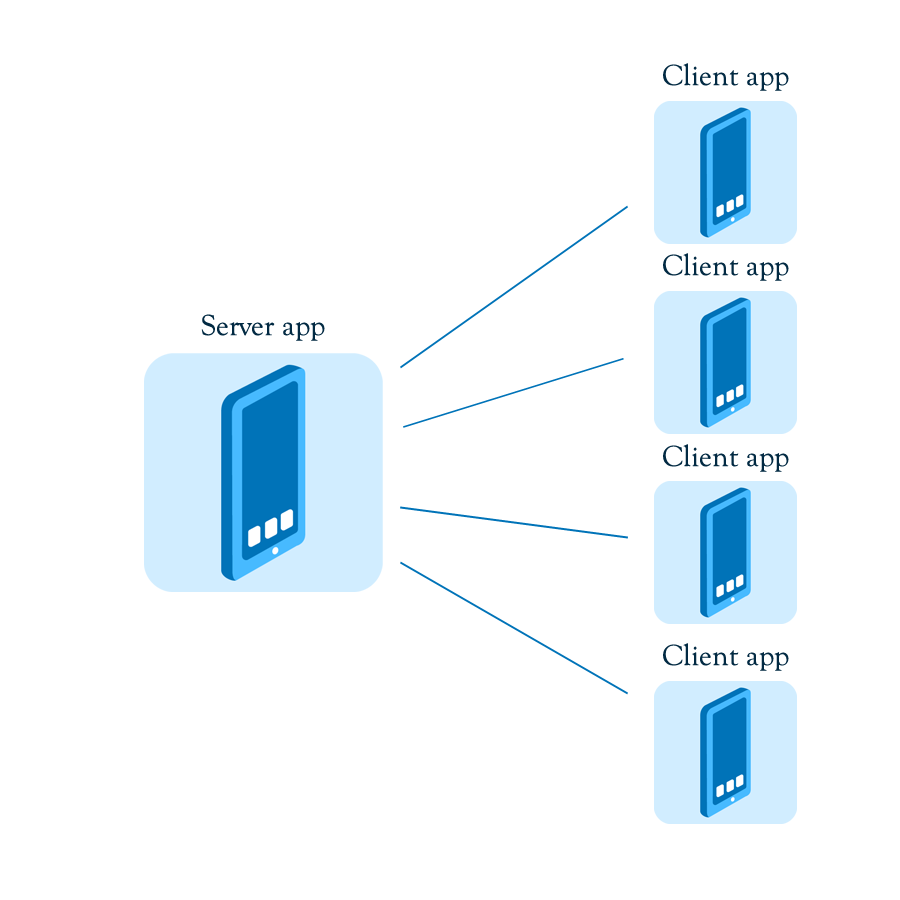
\includegraphics[width=7cm]{sprint1/arhitecture.png}
	\caption{Client-server architecture}
	\label{fig:sprint1_arhitecture}
\end{figure}

\subsection{Logical View}
Figure \ref{fig:class_diagram_client} gives an overview of the client class structure and collaboration. As planed client have all of the functionality covered by user stories. 

\begin{figure}[H]
	\centering
		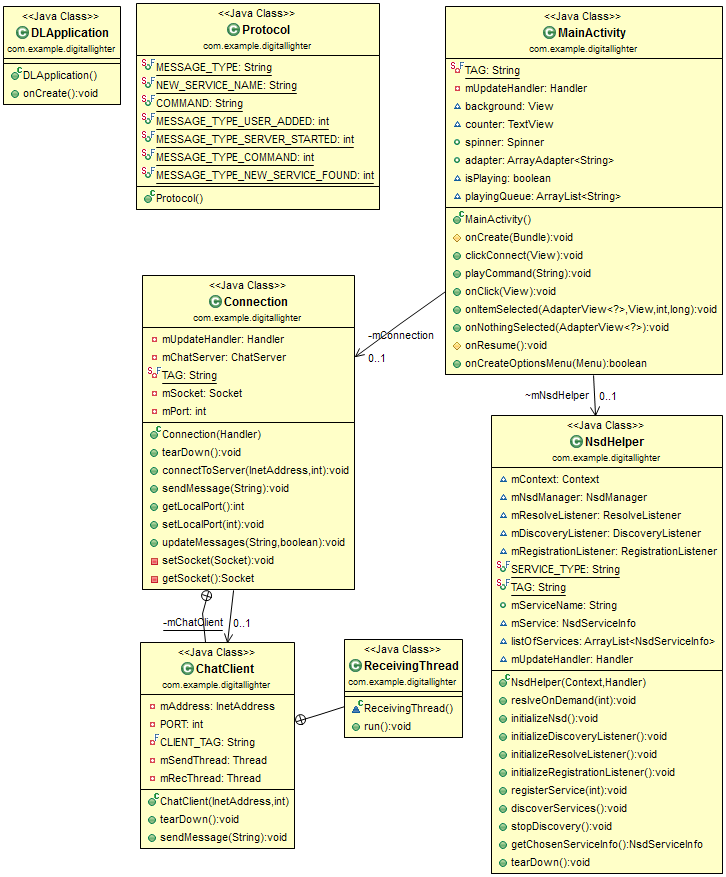
\includegraphics[width=15cm]{sprint1/class_diagram_client.png}
	\caption{Sprint 1 client class diagram}
	\label{fig:class_diagram_client}
\end{figure}

Figure \ref{fig:class_diagram_server} gives an overview of the server class structure and collaboration. Separated thread "ServerThread" for incoming clients was made to optimize server. Sending command signals is also moved from UI thread to "SendingThread" in order to make application more responsive.

\begin{figure}[H]
	\centering
		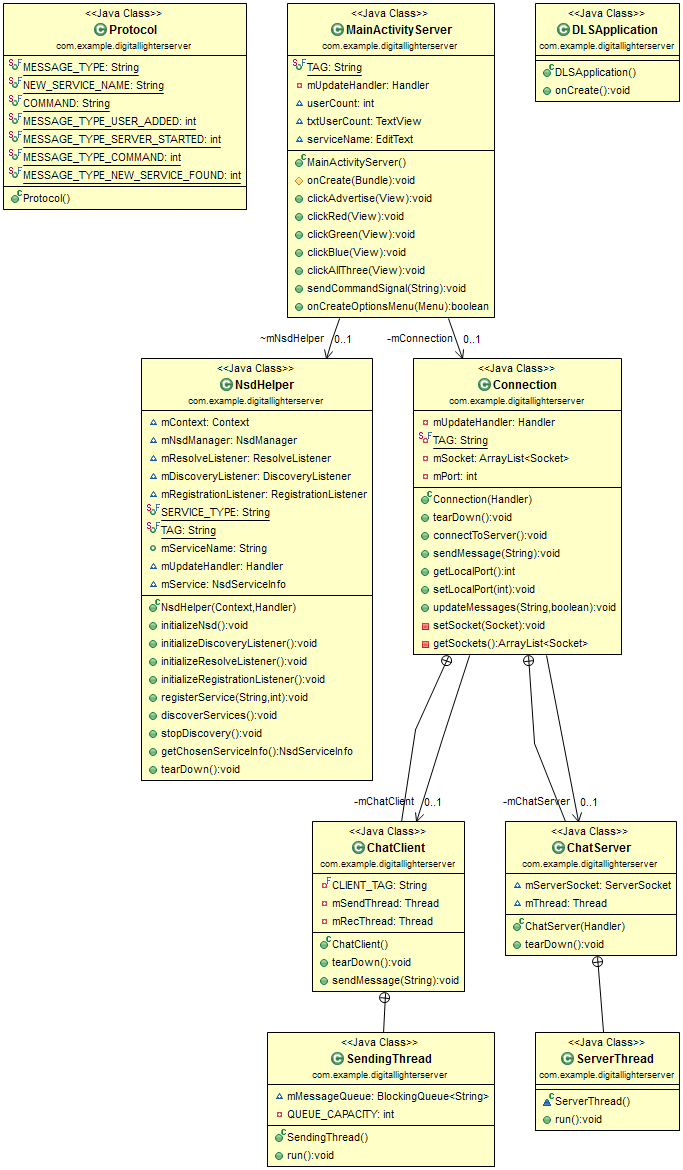
\includegraphics[width=16.2cm]{sprint1/class_diagram_server.png}
	\caption{Sprint 1 server class diagram}
	\label{fig:class_diagram_server}
\end{figure}

On the sequence diagram in Figure \ref{fig:sprint1_communication} it is shown how applications can be used. It gives an idea of how the data flows between different parts of the system when it is up and running.

\begin{figure}[H]
	\centering
		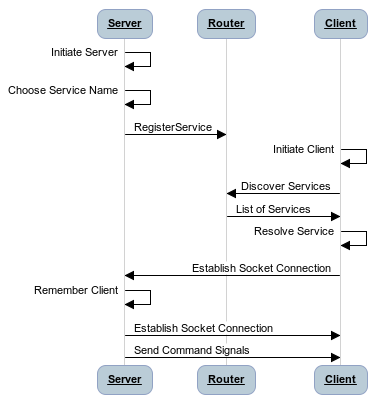
\includegraphics[width=9cm]{sprint1/communication.png}
	\caption{Sprint 1 Communication}
	\label{fig:sprint1_communication}
\end{figure}

\subsection{Physical View}
The deployment diagram, displayed in Figure \ref{fig:deployment_diagram} describes the system architecture focusing on the large components and their connections.

\begin{figure}[H]
	\centering
		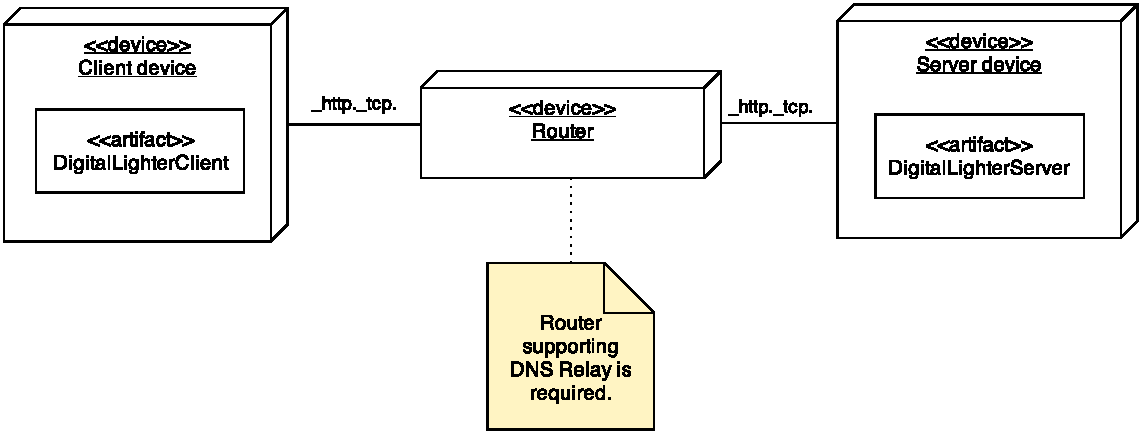
\includegraphics[width=15cm]{images/deployment-diagram-sprint1}
	\caption{Deployment diagram}
	\label{fig:deployment_diagram}
\end{figure}

\paragraph{Client}
is the application that runs on audience Android device. It is able to discover available services, connects to the one and receives command signals from the server. After receiving commands the client is able to flash screen according to given signal.

\paragraph{Router}
is inevitable part of client-server communication since project is based on wireless network and zeroconf technologies. In order to support all of the demands it has to include a DNS relay service. The relay embraces storing of service names and allows look-up stored data to the clients.

\paragraph{Server}
is the application that runs on manager's Android device. It has to register service it provides at router DNS table. Once registered it have to be able to listen for the clients and broadcast command signals to them.


\section{Implementation}

In this sprint most of the work have be done on time. Actual progress was not ideal, but team managed to finish all of the goals that have been set on the beginning of the sprint.
Actual burn down chart can be seen on Figure \ref{fig:Burn1}.  

\begin{figure}[H]
	\centering
		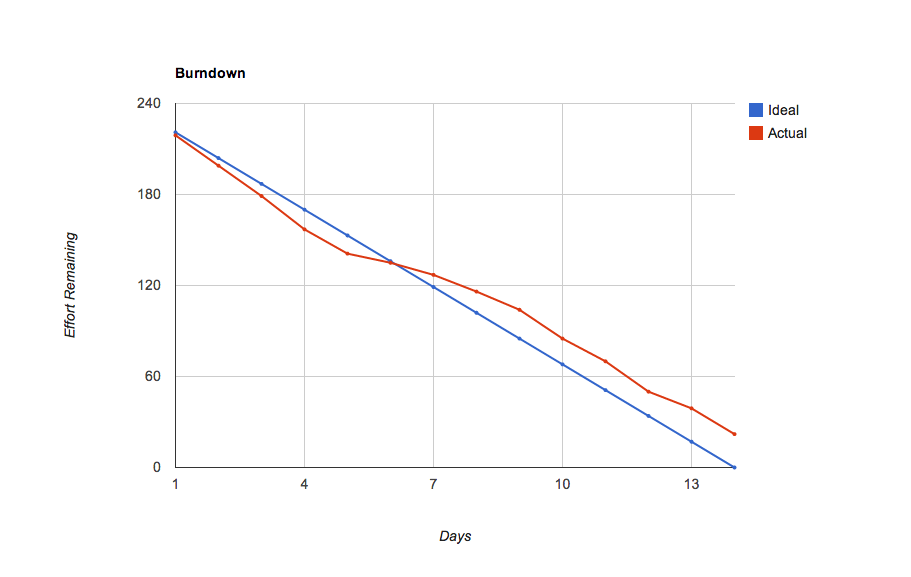
\includegraphics[width=18cm]{sprint1/BurndownSprint1.png}
	\caption{Burn down chart}
	\label{fig:Burn1}
\end{figure}


\section{Occurring risks}
The risk table 3.3, taken from the risk management section in the planning chapter, shows the risks that can occur this project. 
For this sprint most of them did not occur. 
This is because the hardest technical parts, which is the image processing, is not scheduled until the upcoming sprints. 

The user stories for this sprint was very clear, and the customer did not change any of them in the last minute. The team overestimated some of the user stories, so pressure with the time frame was not experienced.

The first risk in the risk table describes team members being sick. This did not occur, but what did occur was that that some of team members had to be absent in some of the working hours. 
The team solved this by having these team members work more independently, and with more flexible hours.  

For now only Android 4.1 adds support for multicast DNS-based discovery.
One of the risks is that Android will not make it available for lower platforms.
In that case a bit over 50\% of the devices will not be supported as shown on the Figure \ref{fig:Platform_chart }, and future development of our prototype will require some of the third part libraries we discovered in prestudy or similar.
Supporting lower platforms in the future, or not, is however never stated in any official document of the Android documentation.

\begin{figure}[H]
	\centering
		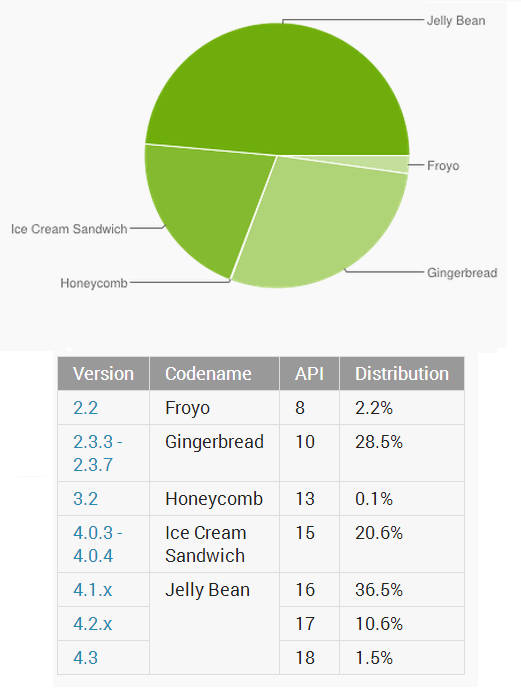
\includegraphics[width=16cm]{sprint1/android_platform_chart.png}
	\caption[Android version distribution]{Android version distribution\footnotemark. Data collected during a 7-day period ending on October 2, 2013. 
	Any versions with less than 0.1\% distribution are not shown}
	\label{fig:Platform_chart }
\end{figure}
\footnotetext{Source: \url{http://developer.android.com/about/dashboards/index.html}}

\section{Customer feedback}
The goal of this sprint was to implement the Prototype 1 as described in Section \ref{txt:planning_productmilestones} but it was not specified how the working increment should be presented to the customer. The team decided to record a demonstration video and present it to the customer through the YouTube online service. The customer was delighted by this idea and encouraged the team to continue in recording the videos for the next demonstrations.

The backlog of user stories was presented to the customer so that he could choose the stories for the next sprint. Since he was satisfied with the team performance during last sprint customer suggested that the team should pick the stories itself as long as the choice suites the intention to finish Prototype 2 until the end of the next sprint.

Customer however disagreed with the time estimated for the single stories contained in the backlog and expressed his concern that the team might be underestimating the complexity of the given tasks. Therefore he changed the time estimated for almost each story by extending it.

The video presented to the customer can be found on YouTube under the name Prototype 1: \url{http://www.youtube.com/watch?v=ofIa5QC6AKA}.

\section{Retrospective}
This section reflects on the past sprint. In order to learn from the mistakes done and thus to improve the workflow it is necessary to answer two essential questions: "What went well" and "What could be improved".

\subsection{What went well}
For the implementation part the sprint 1 goals were reached. The working demonstration video over core client-server module was delivered. The server side registers services, listens for the client, and sends simple  signals. The client is scanning for the services, connecting, receiving signals and play commands on the client. The customer was very satisfied with the video, and suggested recording our future prototypes as well. Besides this we reached the goal to implement Test-Flight in both applications. We also reached the milestone, Obedient client -- Prototype 1.

For the documentation the work done is in the report is good. The report is better structured now, and it actually looks like a report, which is good. The supervisor liked the structure as well. A lot of sections were added when the team integrated the project plan in the report, so that the introduction, the preliminary studies and the planning chapter would be as complete as possible. In for example the preliminary studies chapter the team has not written all of the studies about the image processing part yet, because the team will research this more in later sprints.

\subsection{What could be improved}
The sprint planning in this sprint could have been better. Some of the implementation user stories were over estimated. To solve this better till next time the team should spend more time doing the planning poker. This makes sure that everyone understands the task better. 

The structure of the report is good, but the number of chapters would probably have to be reduced. The supervisor suggested to move the test plan chapter in the planning chapter, since it was such a small chapter. The supervisor also wanted the team to work more with the requirements chapter. There should be a better connection between the user stories and the requirements.


Another con this sprint was that when the product was tested on the mobiles there were problems with the network. Since the mobiles were on different subnets, the client could not find the server. We had to borrow a router and bring with us to be able to test. 



\chapter{Sprint 2}
In this chapter the planning and work-flow regarding Sprint 2 will be described. 
Everything from setting the goals to implementation, and testing. At the end there will evaluate whole sprint, and answers to following questions: What went well? What could be improved? What should we start doing? 

\section{Sprint planning}
The customer was very satisfied with the demonstration video for sprint 1, and suggested recording future prototypes as well. 
After the successful sprint 1 review, the planning of next sprint was started. 
Since the customer was very happy with the sprint 1 delivery, he gave the team an opportunity to decide for themselves what they want to work on in sprint 2, and then ask for his approval.
It has been decided by the team to focus on multiple client support, and since sprint 1 just focused on connecting one client to the server, then it would also be a good opportunity to refine the code which was implemented so far. 
The customer thought this was a really good idea, because working on this now could help in future. 
Catching problems in early phases is much better than discovering them too close to the deadline. 
Then it might not be possible to have enough time to fix those problems.
Therefore sprint 2 will focus on adding support for multiple clients connection and sending different signals to different clients. 
Existing code should be revised and improved so that in next sprint the main effort can be focused on image processing module.


In the supervisor meeting the day after the sprint review, the project report draft was shown to supervisor. 
He was satisfied with the new structure, but he wanted the team to finish more sections. He also insists on creating a work break down structure for the project. 
There were also some chapters that could be merged, which means we should refine the structure of the report. 
These suggestions were included into the sprint plan and according to time estimation some stories were adjusted.

\subsection{Duration}
This Sprint will be 2 weeks long. From 16.09.2013 to 29.09.2013.
The team agreed on the date of presentation and showing the running demo -- Thursday 26.09.2013.
Estimated velocity is 240h since team agreed on 30 working hours per person per week.

\subsection{User-stories}

\subsubsection*{Implementation}
All the functional requirements for sprint 2 are presented in table \ref{tab:sprint2stories}
\LTXtable{\textwidth}{sprint2/stories.tex}

\subsubsection*{Documentation}
All the documentation stories for sprint 2 are presented in table \ref{tab:sprint2Documentationstories}
\LTXtable{\textwidth}{sprint2/storiesDocumentation.tex}

\subsubsection*{Project management}
All the project management stories for sprint 2 are presented in table \ref{tab:sprint2storiesProcess}
\LTXtable{\textwidth}{sprint2/storiesProcess.tex}

% hous all in total: Estimated: 57+104+50= 211 Spent: 48+102 +43 = 193
\section{Sprint Goals}
The goal for Sprint 2 is to deliver a working demo with a more refined core client-server module. 
This still includes registering services, listening for the client and sending simple signals to the client from the server application, but with a more refined code. 
Of course the client should still scan for the services, connect, receive signals, and play the commands. 
The goal is still to use the established simple communication protocol. 
All of the above is extended so it works for several clients connected to the server.

Goals about the report are to refine the report and write the sections needed to be up to speed with the report. This means that sprint 1 chapter has to be finished same as sprint 2 chapter. 

\section{System Burndown}
\begin{figure}[H]
	\centering
		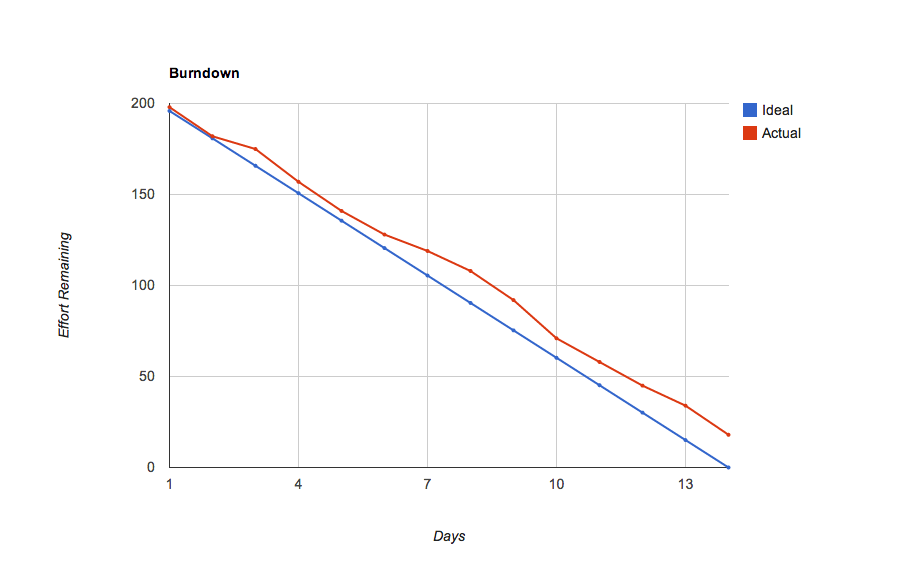
\includegraphics[width=18cm]{sprint2/BurndownSprint2.png}
	\caption{Burn down chart.}
	\label{fig:Burn2 }
\end{figure}

\section{Architecture}
\section{Implementation}
\section{Testing}
\section{Occurring risks}

The risk table \ref{tab:risks} shows many different risks that can occur. 
For this sprint most of them did not occur. 
This is because the most challenging technical parts are not developed yet. 
This is scheduled for sprint 3. 

The user stories for this sprint were also very clear, and really not that different from the last sprint. 
The only difference was that instead of one client, there are now several clients connected to the server. 
As mentioned earlier the customer was very happy with the demonstration in sprint 1, and he let the team choose the stories for this sprint. 
He approved the chosen stories, and because of this no changes in requirements were not met in the last minute.
 
In this sprint the team also did a better job with the time estimation. 
All of this avoids a lot of issues, which is advantage. 
  
\section{Customer feedback}

\section{Retrospective}
This section reflects on the past sprint. In order to learn from the mistakes done and thus to improve the workflow it is necessary to answer two essential questions: "What went well" and "What could be improved".

\subsection{What went well}
The team reached the sprint 2 goals. 
The team delivered the demo with more refined code, and as planned this code supported multiple clients. 
The clients were able to play the commands the server sent.
Another milestone was reached -- Obedient crowd -- Prototype 2.

The work done in the report is very good -- the report is better structured now.
Some extra hours were spent on going through the whole report. 
This was to see if we need to add more in the specific sections, or if we should remove something.  

Even though some members had other responsibilities, and had to absent in some of the working hours, the team still got everything from implementation part done in time for the sprint review. Everyone worked really well independently, as well as in team. 

%The sprint planning in this sprint went really well. 
%We had a perfect amount of work, and the hours estimated for each task, was very realistic, so that was good. 


\subsection{What could be improved}
%The time tracking of each task could have been done better. 
%Even though the team members track their own time, the TargetProcess3 program dos not have a feature for manually edit the time tracking. 
%This means if we forget to do it right away, then the burn down chart wont be as reliable. 
%Since this shows our time tracking we should try to be better at that.

When there is work that needs to be done in the report, the person who writes this section should read terminology, or what other team members have written earlier. 
This will help to get a better flow for the reader.
This will also save a couple of hours when refining is needed afterwards. 


\chapter{Sprint 3}
In this chapter planning and work-flow regarding Sprint 3 will be described. 
All from setting our goals to implementation and testing. On the end we will evaluate whole sprint and try to answer on following questions: What went well? What could be improved? What should we start doing?  
% TODO rewrite

\section{Sprint planning}
In the planning part of sprint 2, there have been introduced and idea or goal for refining and extending the existing code, customer agreed, with condition, that sprint 3 will be focused on image processing part.

As the image processing module was one of the major risks, there was done some preliminary research even in the end of sprint 2 about possible approaches.
One specific way to deal with the problem (using OpenCV and Hough transformation \cite{Duda:1972:UHT:361237.361242}) was introduced to customer in planning part of meeting.
Customer was not satisfied with such a low-level approach and wanted us to use some existing tools.
Therefore there was need for additional preliminary studies concerning existing projects or libraries that could be used.
You can read more about additional preliminary studies below.

Also there was made a proposal of additional "pre-demo" video showing the progress of implementation on Thursday 4th of October 2013 during the regular meeting and customer gladly accepted this offer.


\subsection{Duration}
This sprint is 2 weeks long. From 30th of September 2013 to 13th of October 2013.
We agreed on the date of presentation and showing the running demo -- on Thursday 11 of October 2013.
Estimated velocity is 240 hours since we agreed on 30 working hours per person per week.

\subsection{User-stories}

\subsubsection*{Implementation}
All the functional requirements for sprint 3 are presented in Table \ref{tab:sprint3stories}
\LTXtable{\textwidth}{sprint3/stories.tex}

\subsubsection*{Documentation}
All the documentation stories for sprint 3 are presented in Table \ref{tab:sprint3Documentationstories}
\LTXtable{\textwidth}{sprint3/storiesDocumentation.tex}

\subsubsection*{Project management}
All the project management for sprint 3 are presented in Table \ref{tab:sprint3storiesProcess}
\LTXtable{\textwidth}{sprint3/storiesProcess.tex}

\section{Preliminary studies}
% TODO

\section{Sprint goal}
The goal of this sprint is having a working application on a mobile phone that can work in two modes.  
Input type and output are for both modes common -- input is an image or video and output is location of detected mobile phones in a given matrix (e.g. 4x4 matrix) with color that mobile's screen is lighting.
In the first mode, real video from mobile's camera will be treated as an input and on the other hand in the second mode mock data (image or video) are treated as an input.

You can see example of input with matrix 2x2 in Figure \ref{img:sprint3_goal}. Appropriate output of image processing and mapping module is: \texttt{\{blue,[0,0]\}, \{red,[1,0]\}, \{green,[0,1]\}}.

\begin{figure}[H]
	\centering
		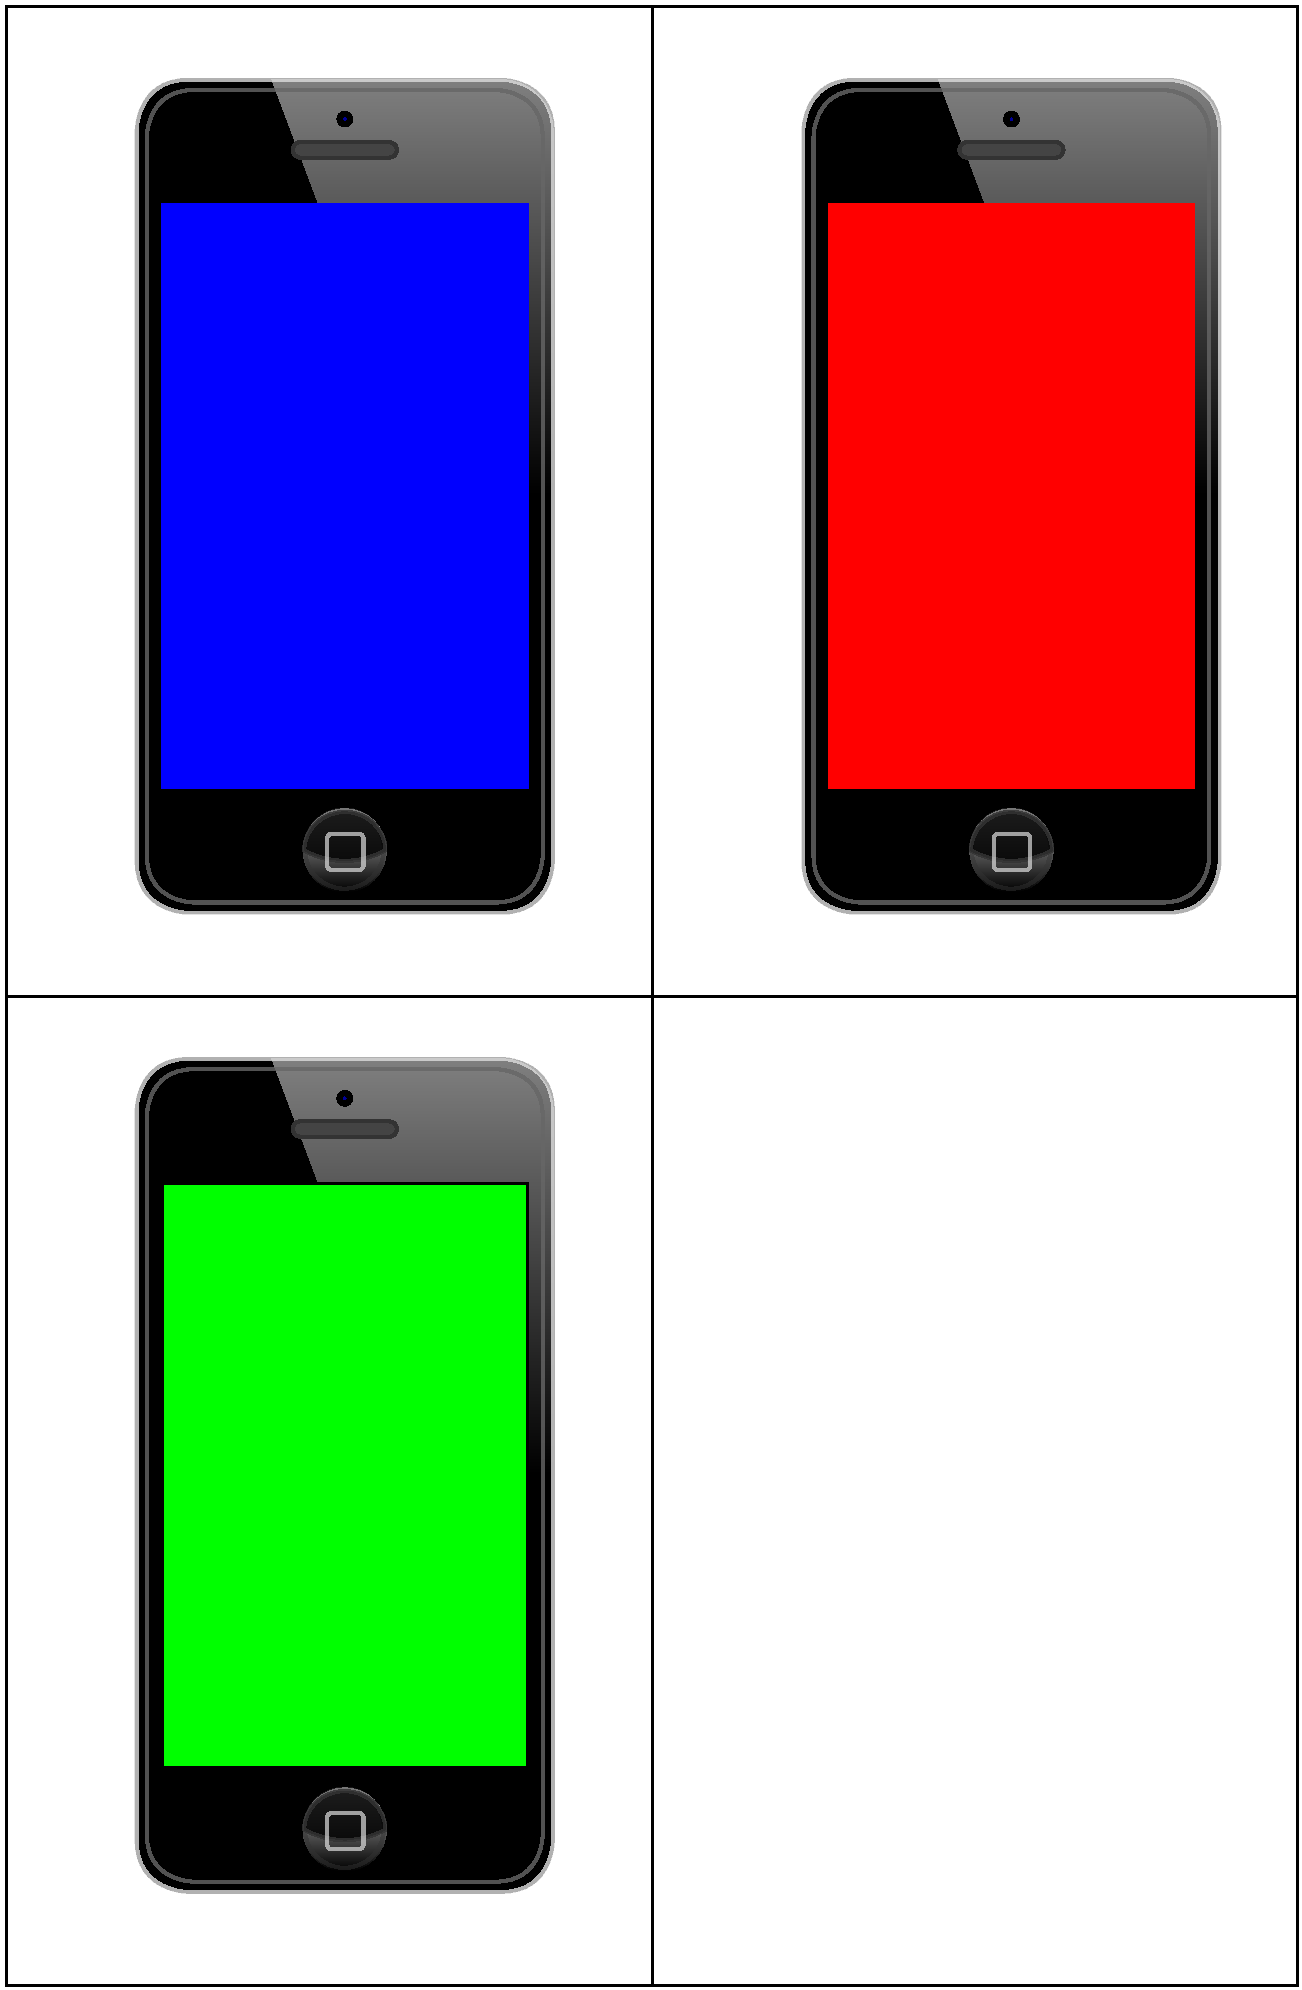
\includegraphics[width=7cm]{sprint3/sprint3_goal.pdf}
	\caption{Example of ideal data input for image processing module with 2x2 matrix.}
	\label{img:sprint3_goal}
\end{figure}


\section{Architecture}
In this section will be described image processing module using 4+1 architectural view module.

\subsection{Logical view}
You can see a class diagram of new classes created in sprint 3 in Figure \ref{fig:class_diagram_sprint3}. We can divide these new classes into three categories. 

Into the first category we count classes \texttt{LightDetector}, \texttt{TileMapper} and \texttt{PointCollector}. 
These classes are a core of image processing module. 
The only visible method for working with this module is \texttt{PointCollector}'s method \texttt{collect}.
This function accepts two parameters: first is the image where mobile phone's screen detection should be done and second is a list of colors of screens which should be detected. 
Method \texttt{collect} is run asynchronously (as a new thread due to possible high time demanding operations) and therefore it was designed as a design pattern \texttt{Observer}
As class \texttt{PointCollector} implements interface \texttt{Observable} (also known as a \emph{Subject} \cite[p.~326]{Gamma:1995:DPE:186897}), its \texttt{Observers} must implement method \texttt{update}. 
To this function is passed as a argument hash map with keys as a colors and values as a lists of tile positions with appropriate color.
Class \texttt{LightDetector} is responsible for detecting location of color blobs in given image. 
Results as a list of pixel's position of blobs are passed as a return value of function \texttt{getBlobCoords}. 
These values are fetched by instance of \texttt{PointCollector} and passed to \texttt{TileMapper}, which is responsible for mapping points into appropriate tiles in grid.

In second category there is only class \texttt{CameraActivity}, who is responsible for handling outputs from camera or mock device and also gives appropriate feedback on screen of mobile (draws grid and marks detected blobs).

In last category there is class \texttt{ColorManager}, which is standalone class and in application there is only need for one instance. Therefore it was designed as a \texttt{Singleton} pattern \cite[p.~144]{Gamma:1995:DPE:186897}. Its main purpose is to handle transformations of different color formats such as special library, network and internal formats.

\begin{figure}[H]
	\centering
		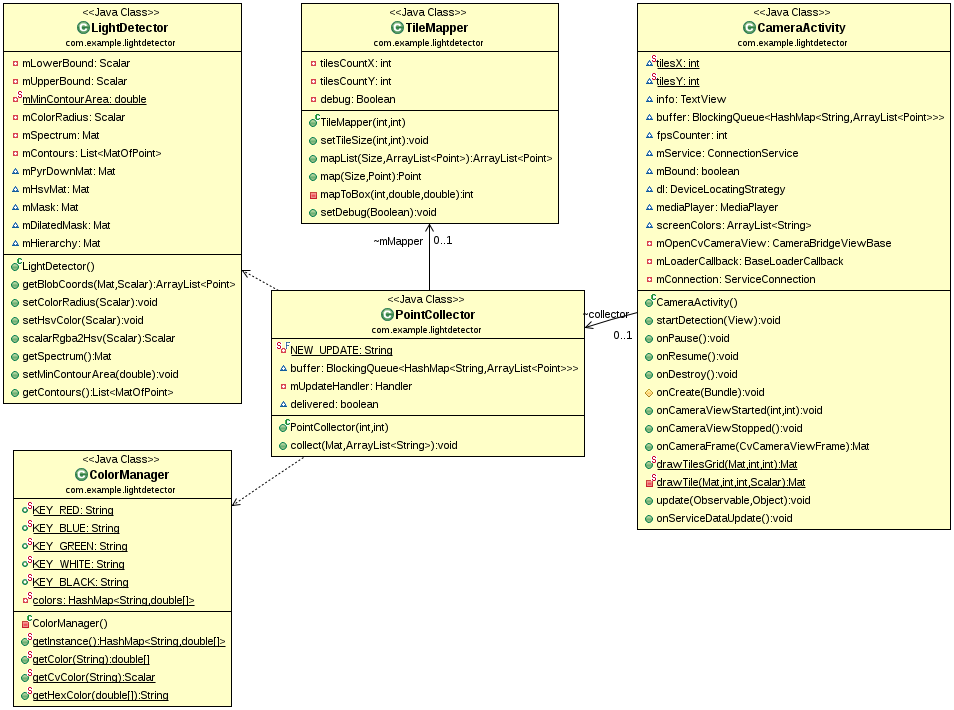
\includegraphics[width=16.2cm]{sprint3/sprint3.png}
	\caption{Sprint 3 light detection module class diagram}
	\label{fig:class_diagram_sprint3}
\end{figure}

\subsection{Physical view}
You can see the physical view of whole product represented in Figure \ref{fig:sprint3_deployment_diagram}.
Even though in this particular case device \emph{Camera} part of \emph{Server} device, the architecture and code was designed generally so \emph{Camera} can be stand alone device.

\begin{figure}[H]
	\centering
		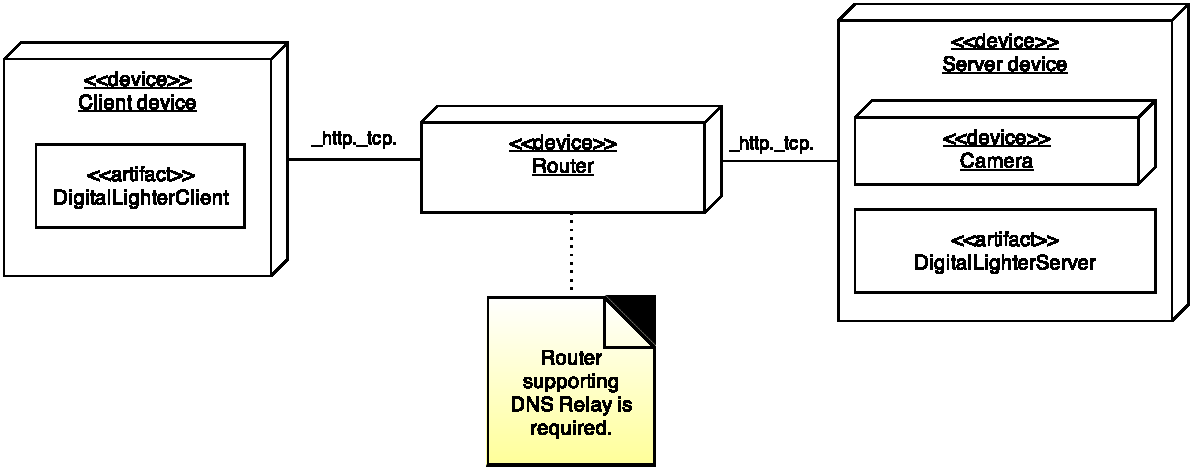
\includegraphics[width=15cm]{images/deployment-diagram-sprint3}
	\caption{Deployment diagram}
	\label{fig:sprint3_deployment_diagram}
\end{figure}

\subsection{Process view}
You can see the process view represented in Figures \ref{fig:sprint3_activity_diagram} and \ref{fig:sprint3_dfd}.
It should be mentioned, that each time new image was taken by camera, new thread is created and therefore several processing in the same time can be performed.

\begin{figure}[H]
	\centering
		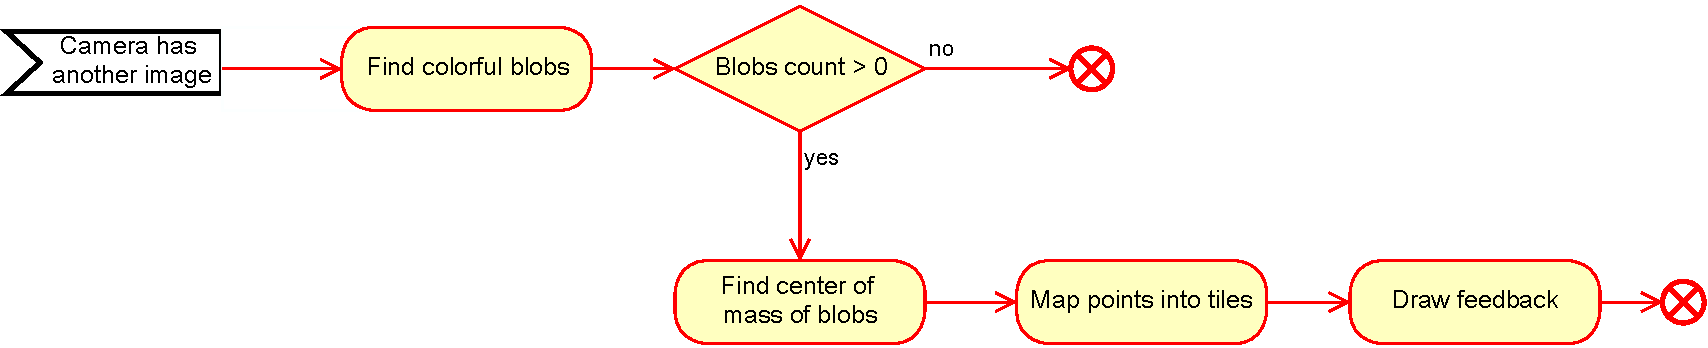
\includegraphics[width=16.2cm]{sprint3/sprint3_activity.pdf}
	\caption{Sprint 3 activity diagram}
	\label{fig:sprint3_activity_diagram}
\end{figure}


\begin{figure}[H]
	\centering
		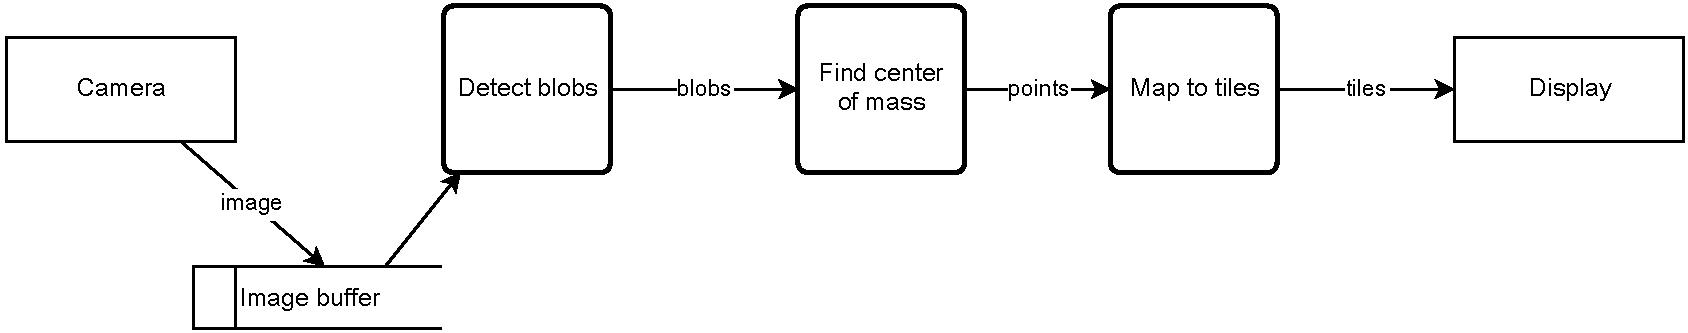
\includegraphics[width=16.2cm]{sprint3/sprint3_dtd.pdf}
	\caption{Sprint 3 data flow diagram}
	\label{fig:sprint3_dfd}
\end{figure}

%\subsection{Development view}
%Since this is a single module, there is no need for development view

\section{Implementation}

Few problems during implementation had occurred. 
Since the OpenCV library for Java is in early stage, there is some functionality missing.
One of these is a method \texttt{open(String)} of class \texttt{VideoCapture}\footnote{http://docs.opencv.org/java/org/opencv/highgui/VideoCapture.html}.
In C++ version of OpenCV there exist such a method and it allows programmers to use a video for input for image processing.
After short research, a fix of this bug was found\footnote{http://code.opencv.org/issues/3207}, but this feature will be added in release 2.4.7.
Due to this discovery, there has been abandoned (at least until OpenCV 2.4.7 is released) a plan for mocking a video and only single pictures were used for testing.


\section{Testing}
A capability of Java to run on multiple platforms were utilized during testing and initial testing was performed without any Android device.
There have been created a testing set\footnote{https://github.com/dohnto/DigitalLighter/tree/master/source/others/LightDetectorTester/res/drawable} of simple images used for black box testing.

After this test, it has been decided to merge module with the rest of the application and perform some integration tests.
To outline a characteristics of further testing you can see videos \footnote{http://www.youtube.com/watch?v=TcuMlvvAwSQ} \footnote{http://www.youtube.com/watch?v=fhWFAJY7QOg} demonstrating current progress of implementation.

\section{Occurring risks}
\section{Retrospective and evaluation}
\subsection{What went right}
Since the preliminary studies concerning image processing started very soon and instead of writing light detection module from scratch an existing code was used, the core of implementation was finished ahead of schedule.

\subsection{What went wrong}
Due to misunderstanding customer's demands regarding using existing solution, extra time was required for additional preliminary studies resulting to the same output as the first preliminary study concerning image processing. 
In the end, the customer approved using OpenCV as a best option.
Therefore the communication with customer should be more precise and accurate and if any ambiguity occurs, it should be consulted with customer as soon as possible.

From the beginning it was obvious, that the light detection module's performance affected by level of light.
During the testing the team was uncertain when the performance is sufficient, because the question of lighting was not discussed enough.
After this experience, an proposal to customer was made: if similar situation occurs, acceptance tests should be prepared and approved by the customer.

Last but not least, documentation stories XX YY ZZ were not finished due to need to refining previously written chapters.
\subsection{What to improve}
As mentioned in previous paragraphs, the communication with customer should be improved.
Also, daily stand ups were often omitted due to late attendance.
Even though the workload is 30 hours per week per person, the efficiently spend time is much more lower, therefore the workload was decreased to 25 hours per week per person.

\chapter{Sprint 4}
In this chapter the planning and work-flow regarding Sprint 4 will be described. 
Everything from setting our goals to implementation and testing. At the end we will evaluate the whole sprint and try on answer the following questions: What went well? What could be improved? 
\section{Sprint planning}

The customer was very satisfied with the demonstration video for sprint 3. The team planned how to take the project further. At this point it was possible to send control signals to multiple clients, and then detect the devices that lit up. We decided that the plan for this sprint was to combine those two, and try to create an image. We wanted to create a traffic light. This meant that after detection, we had to send signals to make the first client light up red, and make the second one light up yellow, and then make the last one light up green. Since the main goal was to make the mobile screens create an image, the order of the different colors was be imporant. We had to plan for making specific devices to light up specific colors at spesific positions. A traffic light was a good start for focusing on this part of the assignment, and the customer agreed. For sprint 4, the plan was to first map all available devices to grid, and then link the devices location with their ids, and then make the clients create a traffic light.  


In sprint 4 the team also planned to work more on the report. Our plan was to finish sprint 3, since that sprint finished the week before. It was also wanted to start working on sprint 4. Since it was implemented detection of devices, and it was planned to link their location to their ids, we figured that we needed to add more information about the software architecture as well. We where also starting to get a better understanding of what the end product would look like, therefore we planned to also start working a little bit on the evaluation. The supervisor also came up with some suggestions for small improvements on the report, which the team planned to follow up. Also it was decided to make to the user stories more consistent. It was also planned to separate the implementation stories from the documentation, and the project management stories.


All implementation related stories for sprint 4 are presented in table \ref{tab:sprint4stories}.
\LTXtable{\textwidth}{sprint4/stories.tex}

All the documentation related stories for sprint 4 are presented in table \ref{tab:sprint4Documentationstories}.
\LTXtable{\textwidth}{sprint4/storiesDocumentation.tex}

All the project management related stories for sprint 4 are presented in table \ref{tab:sprint4storiesProcess}.
\LTXtable{\textwidth}{sprint4/storiesProcess.tex}

% hous all in total: Estimated: 130 + 65 + 42 = 237  Spent: 136+ 36+35= 207

\subsection{Duration}
This sprint is 2 weeks long. From 14th of October 2013 to 27th of October 2013. We agreed
on the date of presentation and showing the running demo – on Thursday 25th of October 2013.
Estimated velocity is 240 hours since we agreed on 30 working hours per person per week.

\section{Preliminary studies}
% TODO
\section{Sprint goal}

The goal for sprint 4 is to link the devices location with their ids, and then make the clients create a traffic light together. 
\begin{figure}[H]
	\centering
		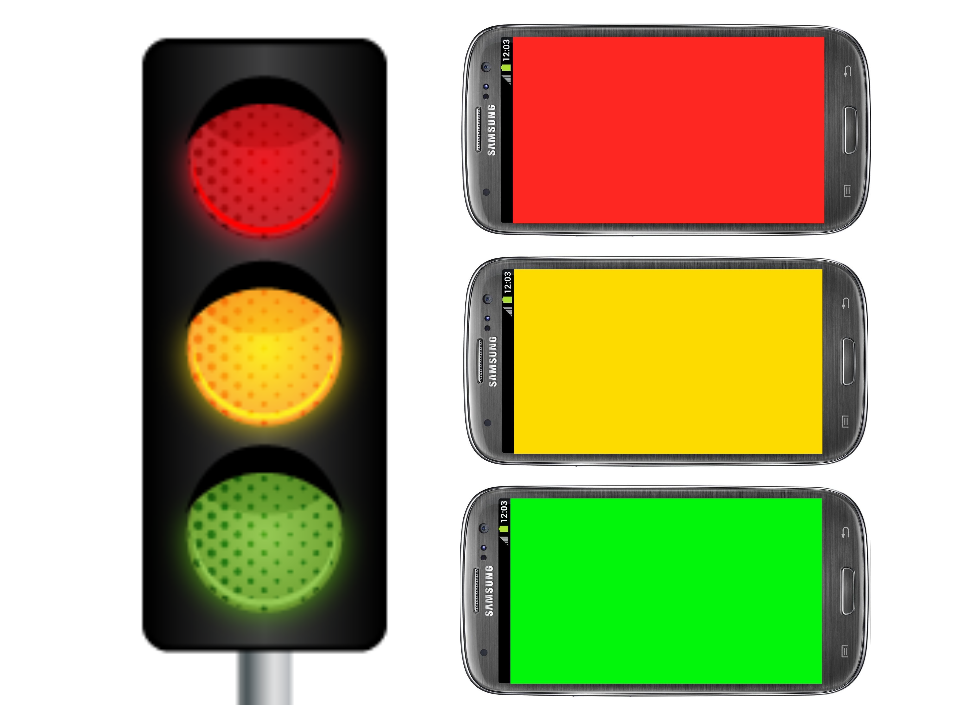
\includegraphics[width=10cm]{sprint4/trafficlight.png}
	\caption{Traffic Light.}
	\label{fig:trafficlight }
\end{figure}

\section{System Burndown}
\begin{figure}[H]
	\centering
		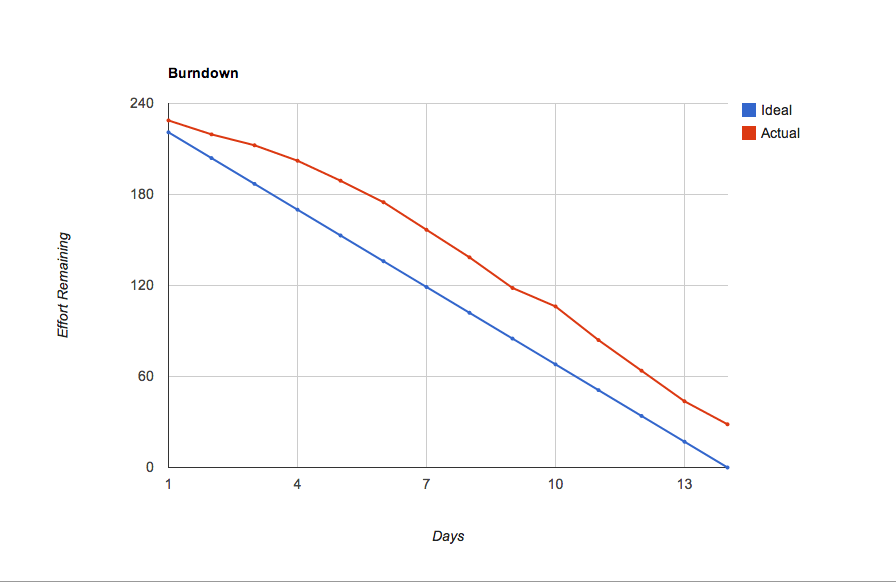
\includegraphics[width=18cm]{sprint4/BurndownSprint4.png}
	\caption{Burn down chart.}
	\label{fig:Burn4 }
\end{figure}
\section{Architecture}
\section{Implementation}
\section{Testing}
\section{Occurring risks}
\section{Customer feedback}
\section{Retrospective}
This section reflects on the past sprint. In order to learn from the mistakes done and thus to improve the workflow it is necessary to answer two essential questions: "What went well" and "What could be improved".

\subsection{What went well}
\subsection{What could be improved}


\chapter{Sprint 5}
As in previous sprint chapters, work-flow trough sprint 5 will be described. What makes this sprint different from the others, is that the team had to manage occurred risk on communication module. A good part of this chapter will be devoted to resolution of risk, but it will not lack the rest of the processes such as planning, establishing goals and retrospective.

\section{Sprint planning}

The planning started with customer meeting at Thursday 24th of October 2013. For the customer, the main event and goal of this sprint, is to finalize the prototype and record the demo video. Therefore planning includes tasks as: collecting phones from friends, researching the companies that do mobile development and borrowing the phones from them, renting the room and recording equipment from university. We planned to borrow phones from friends, but if that did not work we planned to borrow phones from companies.

The recording final demo is planned for Thursday 7th of November, and informing potential phone owners that will be able to share their phones with us is planned at least one week before the event. This way table of potential phones can be crated, and risk of not collecting the sufficient number of devices can be reduced and solved. Recording equipment is planned to be rented or reserved at least 3 days before the event.

As far as the implementation is concerned the team focused mainly on device detection part as the customer required to speed up this process. In order to achieve this task the \textit{tree algorithm} for detection was developed (see Section \ref{txt:sprint5_immplementation}). We planned that the final demo would show an equalizer since the theme for the whole project was a rock concert. Therefor we also needed to implement a predefined gallery.
In sprint 5 we plan to work further on the report. Our plan is to finish sprint 4, and sprint 5. We also need to work further on the evaluation and the conclusion chapters.  

All implementation related stories for sprint 5 are presented in Table \ref{tab:sprint5stories}.
%\caption{User stories selected for Sprint 4.}
  \label{tab:sprint4stories}
 \def\arraystretch{1.25}
 
\begin{longtable}{ccXcc}

\toprule[0.5mm]
\multirow{2}{*}{\textbf{ID}} &
\multirow{2}{*}{\textbf{Ref.}} & \multirow{2}{*}{\textbf{Description}} & \multicolumn{2}{c}{\textbf{Hours}} \\
 					& & & \textbf{Est.} & \textbf{Sp.} \\
%\textbf{ID} 	& \textbf{Description} 	& \textbf{Est.} & \textbf{Sp.} \\
\midrule
\textbf{I4.1} 	& 	& {\bf As a server I need to link the devices' location with their ids.}	 &  52	& \textbf{48} \\

\textbf{I4.2} 	& 	& {\bf As a server I need to identifiy multiple clients from light.}		 &  19	& \textbf{18} \\

\textbf{I4.3} 	& 	& {\bf As a server I need to map all available devices to grid.} 			 & 22 & \textbf{18} \\	

\textbf{I4.4} 	& 	& {\bf As a server I need to play the whole media to the grid.} 			 & 37 & \textbf{34} \\
	
\midrule
		
				&& \textbf{SUM:}		&		130	& \textbf{136}
 \\																			
\bottomrule[0.5mm]
\end{longtable}


All the documentation related stories for sprint 5 are presented in Table \ref{tab:sprint5Documentationstories}.
%\caption{User stories selected for Sprint 2.}
\def\arraystretch{1.25}
 
\begin{longtable}{ccXcc}
\label{tab:sprint2Documentationstories}\\[-6mm]
\caption{Documentation stories selected for sprint 2}\\[-4mm]
\toprule[0.5mm]
\multirow{2}{*}{\textbf{ID}} &
\multirow{2}{*}{\textbf{Ref.}} & \multirow{2}{*}{\textbf{Description}} & \multicolumn{2}{c}{\textbf{Hours}} \\
 					& & & \textbf{Est.} & \textbf{Sp.} \\
%\textbf{ID} 	& \textbf{Description} 	& \textbf{Est.} & \textbf{Sp.} \\
\midrule


\textbf{D2.1} 	& 
	\refwbs{wbs_documentation}{WBS 8.2}	& {\bf As a student I need to finish the pre-study chapter.} 									& 	12	& \textbf{ 16} \\

\textbf{D2.2} 	& 
	\refwbs{wbs_documentation}{WBS 8.2}	& {\bf As a student I need to finish the planning chapter.} 									& 	10	& \textbf{ 14} \\

\textbf{D2.3} 	&
	\refwbs{wbs_documentation}{WBS 8.2} 	& {\bf As a student I need to finish requirements chapter.} 									& 	30	& \textbf{ 26} \\

\textbf{D2.4} 	& 
	\refwbs{wbs_documentation}{WBS 8.2}  & {\bf As a student I need to finish the architecture chapter.} 								& 	24	& \textbf{ 12} \\

\textbf{D2.5} 	& 
	\refwbs{wbs_documentation}{WBS 8.2}	& {\bf As a student I need to finish sprint 1 chapter.} 										& 	12	& \textbf{ 16} \\

\textbf{D2.6} 	& 
	\refwbs{wbs_documentation}{WBS 8.2}	& {\bf As a student I need to work on the  sprint 2 chapter.} 									& 	16	& \textbf{ 18} \\
%ASK group about this:
%\textbf{360} 	& \refreq{}
%	& {\bf As a student I need to start on the architechture chapter.} 								& 	?	& \textbf{ ?} \\	

								
\hline
				&& \textbf{SUM:}		&		104	& \textbf{102}
 \\																			
\bottomrule[0.5mm]
\end{longtable}

All the project management related stories for sprint 5 are presented in Table \ref{tab:sprint5storiesProcess}.
%\caption{User stories selected for Sprint 1.}
\label{tab:sprint1storiesProcess}
\def\arraystretch{1.25}
 
\begin{longtable}{ccXcc}

\toprule[0.5mm]
\multirow{2}{*}{\textbf{ID}} &
\multirow{2}{*}{\textbf{Ref.}} & \multirow{2}{*}{\textbf{Description}} & \multicolumn{2}{c}{\textbf{Hours}} \\
 					& & & \textbf{Est.} & \textbf{Sp.} \\
%\textbf{ID} 	& \textbf{Description} 									& \textbf{Est.} & \textbf{Sp.} \\
\midrule

% === Process ==========================
\textbf{326} 	& 
	& {\bf  As a student I have to track effort time} 	& 		16	& \textbf{16} \\
\textbf{345} 	& 
	& {\bf As a student I have attend the weekly meetings with the customer} 	
	& 	22	
	& \textbf{?} \\
		&& Preparation for demonstration	& 2 & ? \\
		&& Demonstration	& 6 & ? \\
		&& Writing minutes 	&  6 & ? \\	
		&& Customer meeting	&  6 & ? \\
		&& Writting minutes	&  2 & ? \\
		
\textbf{327} 	& 
	& {\bf As a student I have to attend the weekly meetings with the supervisor} 	
	& 	12	
	& \textbf{?} \\
		&& Meeting in week I	& 4 & ? \\
		&& Meeting in week II	& 4 & ? \\
		&& Writing minutes from week I 	&  2 & ? \\
		&& Writing minutes from week II	&  2 & ? \\	

\textbf{344} 	&& {\bf As a student I need to attend the team building.} 	& 		7	& \textbf{9} \\
		

\textbf{321} 	&& {\bf As a student I need to participate to lectures about team dynamics. } 	& 		32	& \textbf{25} \\
				&& Course of group dynamics Thu.	&  &  \\
				&& Summary of course and exchange learned.	&  &  \\				
				
\hline
				&& \textbf{SUM:}		&		164	& \textbf{?}
 \\																			
\bottomrule[0.5mm]
\end{longtable}


% hous all in total: Estimated: 235  Spent: 230


\subsection{Duration}
This sprint is 2 weeks long. From 28th of October 2013 to 10th of November 2013. We agreed
on the date of presentation and showing the running demo – on Thursday 7th of November 2013.
Estimated velocity is 240 hours since we agreed on 30 working hours per person per week. 


\section{Sprint Goal}

On the end of this sprint team expect to have working, the prove of concept demo. As core modules are finished, team will invest time in tuning existing and implementing some of the supporting functionalities. Some of them are: speeding up the detection process  and preparing predefined gallery to be played. Goal for this sprint is also a time sync between server and clients. Reason is bypassing possible networking latency, and enabling clients to play the content more precise. 

\section{Duration}
This sprint is 2 weeks long. From 28th of October 2013 to 10th of November 2013. 
Team agreed on the date of presentation and showing the running demo – on Thursday 7th of November 2013.
Estimated velocity is 200 hours since every team member will devote 25 working hours per week.

\section{Architecture}

At first team was thinking about implementing the clock synchronization from scratch. Using one of the popular algorithms as Berkeley algorithm\footnote{\url{http://ieeexplore.ieee.org/stamp/stamp.jsp?tp=\&arnumber=29484}}, and adding additional responsibility to server or client application. 

The Berkeley algorithm requires feedback communication from clients by implementing receiving message system on server. Calculating the time offset on server and adjusting local times on clients. The protocol will have to expended in order to support clock sync communication. Although this approach will work, lot of changes on existing architecture have to be done.

As focus of this project is on proving the concept, and time for big implementation parts or structure changes is not sufficient, team agreed on researching alternative solutions before start implementing. This is also part of Risk management strategy where team have to be careful not to implement things they are not suppose to, according to Table \ref{tab:risks}. Further research has brought the team to Network Time Protocol (NTP)\footnote{\url{https://tools.ietf.org/html/rfc5905\#section-14}}.

Good thing about NTP is that it is used for variable-latency data networks. It was only needed to find application that provide NTP service, and change client code to call this service and determine what is a local time offset before connecting to Digital Lighter server application. In that case, change of existing architecture will be minimal, and it will play only on client application. No server, or protocol will have to be changed.

As solution Time Server\footnote{\url{https://play.google.com/store/apps/details?id=com.icecoldapps.timeserver}} application have been chosen. It will work on same device as Digital Lighter server application, and it will provide same time as Digital Lighter application would. Deployment digram is therefore changed, and now includes NTP server as artifact. 

\begin{figure}[H]
	\centering
		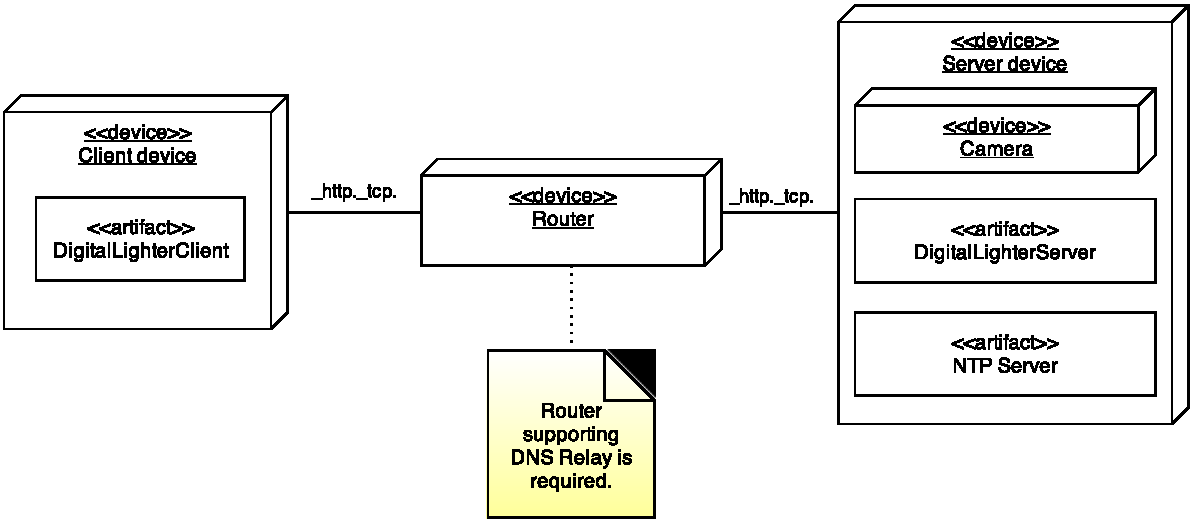
\includegraphics[width=15cm]{images/deployment-diagram-sprint5}
	\caption{Deployment diagram}
	\label{fig:sprint5_deployment_diagram}
\end{figure}

Change have influence on messages interchange between server and clients. The difference comparing to old sequence diagram is given at Figure \ref{fig:sprint5_sequence_diagram}. New calls are colored red. 

\begin{figure}[H]
	\centering
		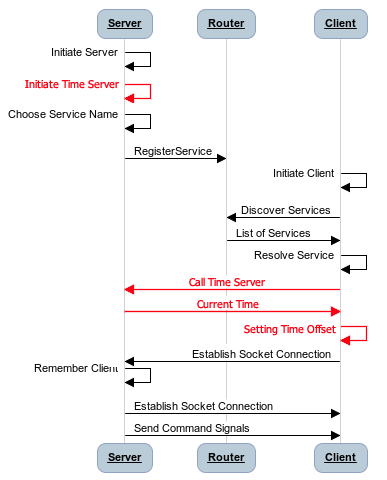
\includegraphics[width=9cm]{sprint5/communication}
	\caption{Sequence diagram}
	\label{fig:sprint5_sequence_diagram}
\end{figure}

Observing deployment and sequence diagrams, it is easy to see that this solution didn't need existing system to change. But in same time new functionality have been added and big amount of time have been saved. This way project architecture follows open/closed principle\footnote{\url{http://msdn.microsoft.com/en-us/magazine/cc546578.aspx}}. System is closed for changes, but open for extensions.

Logical view of added module is shown in Figure \ref{fig:Time_Sync_class }. Class \texttt{SNTPClient} makes call to time server in separate thread, and in \texttt{doInBackground} method retrieve NtpMessage object in order extract exact time from server. \texttt{NtpMessage} represents a NTP message, as specified in RFC 2030\footnote{\url{http://www.rfc-base.org/txt/rfc-2030.txt}}. The message format is compatible with all versions of NTP and SNTP. This class does not support the optional authentication protocol, and ignores the key ID and message digest fields. For convenience, this class exposes message values as native Java types, not the NTP-specified data formats. For example, timestamps are stored as doubles (as opposed to the NTP unsigned 64-bit fixed point format). However, the constructor NtpMessage(byte[]) and the method toByteArray() allow the import and export of the raw NTP message format.

\begin{figure}[H]
	\centering
		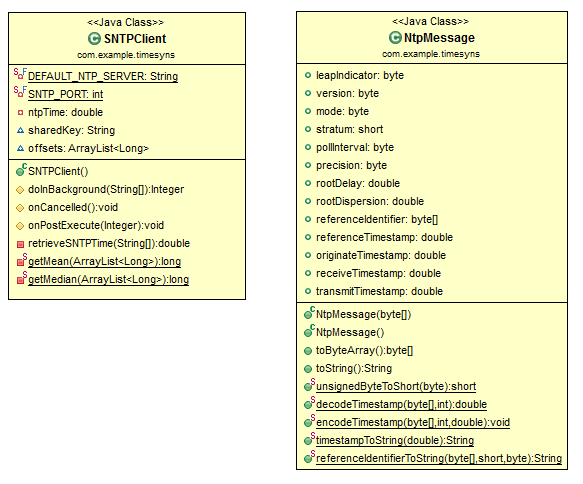
\includegraphics[width=14cm]{sprint5/sprint5_class_diagram.png}
	\caption{Time sync class diagram}
	\label{fig:Time_Sync_class }
\end{figure}

\section{Implementation} \label{txt:sprint5_immplementation}
This section is devoted to describing the improved algorithm used for faster detection of the devices. So far the simple detection using "one-by-one" approach as explained in Section \ref{txt:sprint4_processview} was used. The drawback of this algorithm is that it performs with time complexity $T(n) = O(n)$ and thus it might get inadmissibly long. Thus more advanced algorithm based on divide and conquer design paradigm was developed. It will be described in greater detail in next sections.

\subsection{Algorithm}
The algorithm is based on the assumption that the image processing module originally designed and implemented during Sprint 3 (see Section \ref{txt:sprint3_architecture}) is capable of recognizing multiple different colors. Then it possible to recursively divide all the devices into the groups of the same color until there is only one device left in each subgroup. This algorithm is referred to as the \textit{tree algorithm} since the recursive divison gradually creates the tree where each node excluding the leaf nodes has $n$ children where $n = number\_of\_colors\_used\_during\_detection$.

Figure \ref{fig:sprint5_tree_alg} depicts the example of the detection process of the 16 devices while recognizing among 4 different colors: red, green, blue, yellow. In this example the ideal conditions where each device precisely fits into one single matrix tile are set. 

One step of the algorithm can be represented as generating the new level of the tree (STEP 0, STEP 1 and STEP 2 in Figure \ref{fig:sprint5_tree_alg}). Given the specific tree level each node represents the group of devices that are to be lit with the same color. Devices are assigned to the groups randomly and it is required that each group would consist of the the same number of devices if possible (otherwise some groups might differ by 1 device).

Once it was decided which device will be lit by which color the server sends relevant signals to all of the devices and then detects the color blobs in the image. It saves the position of detected colors and proceeds to the next step.

The algorithm ends when there are is no more than one device in each color group. Then the saved history of the colors sent to each device can be compared to the actual detected colors and their positions which results in detecting the real position of each device.

\begin{figure}[H]
	\centering
		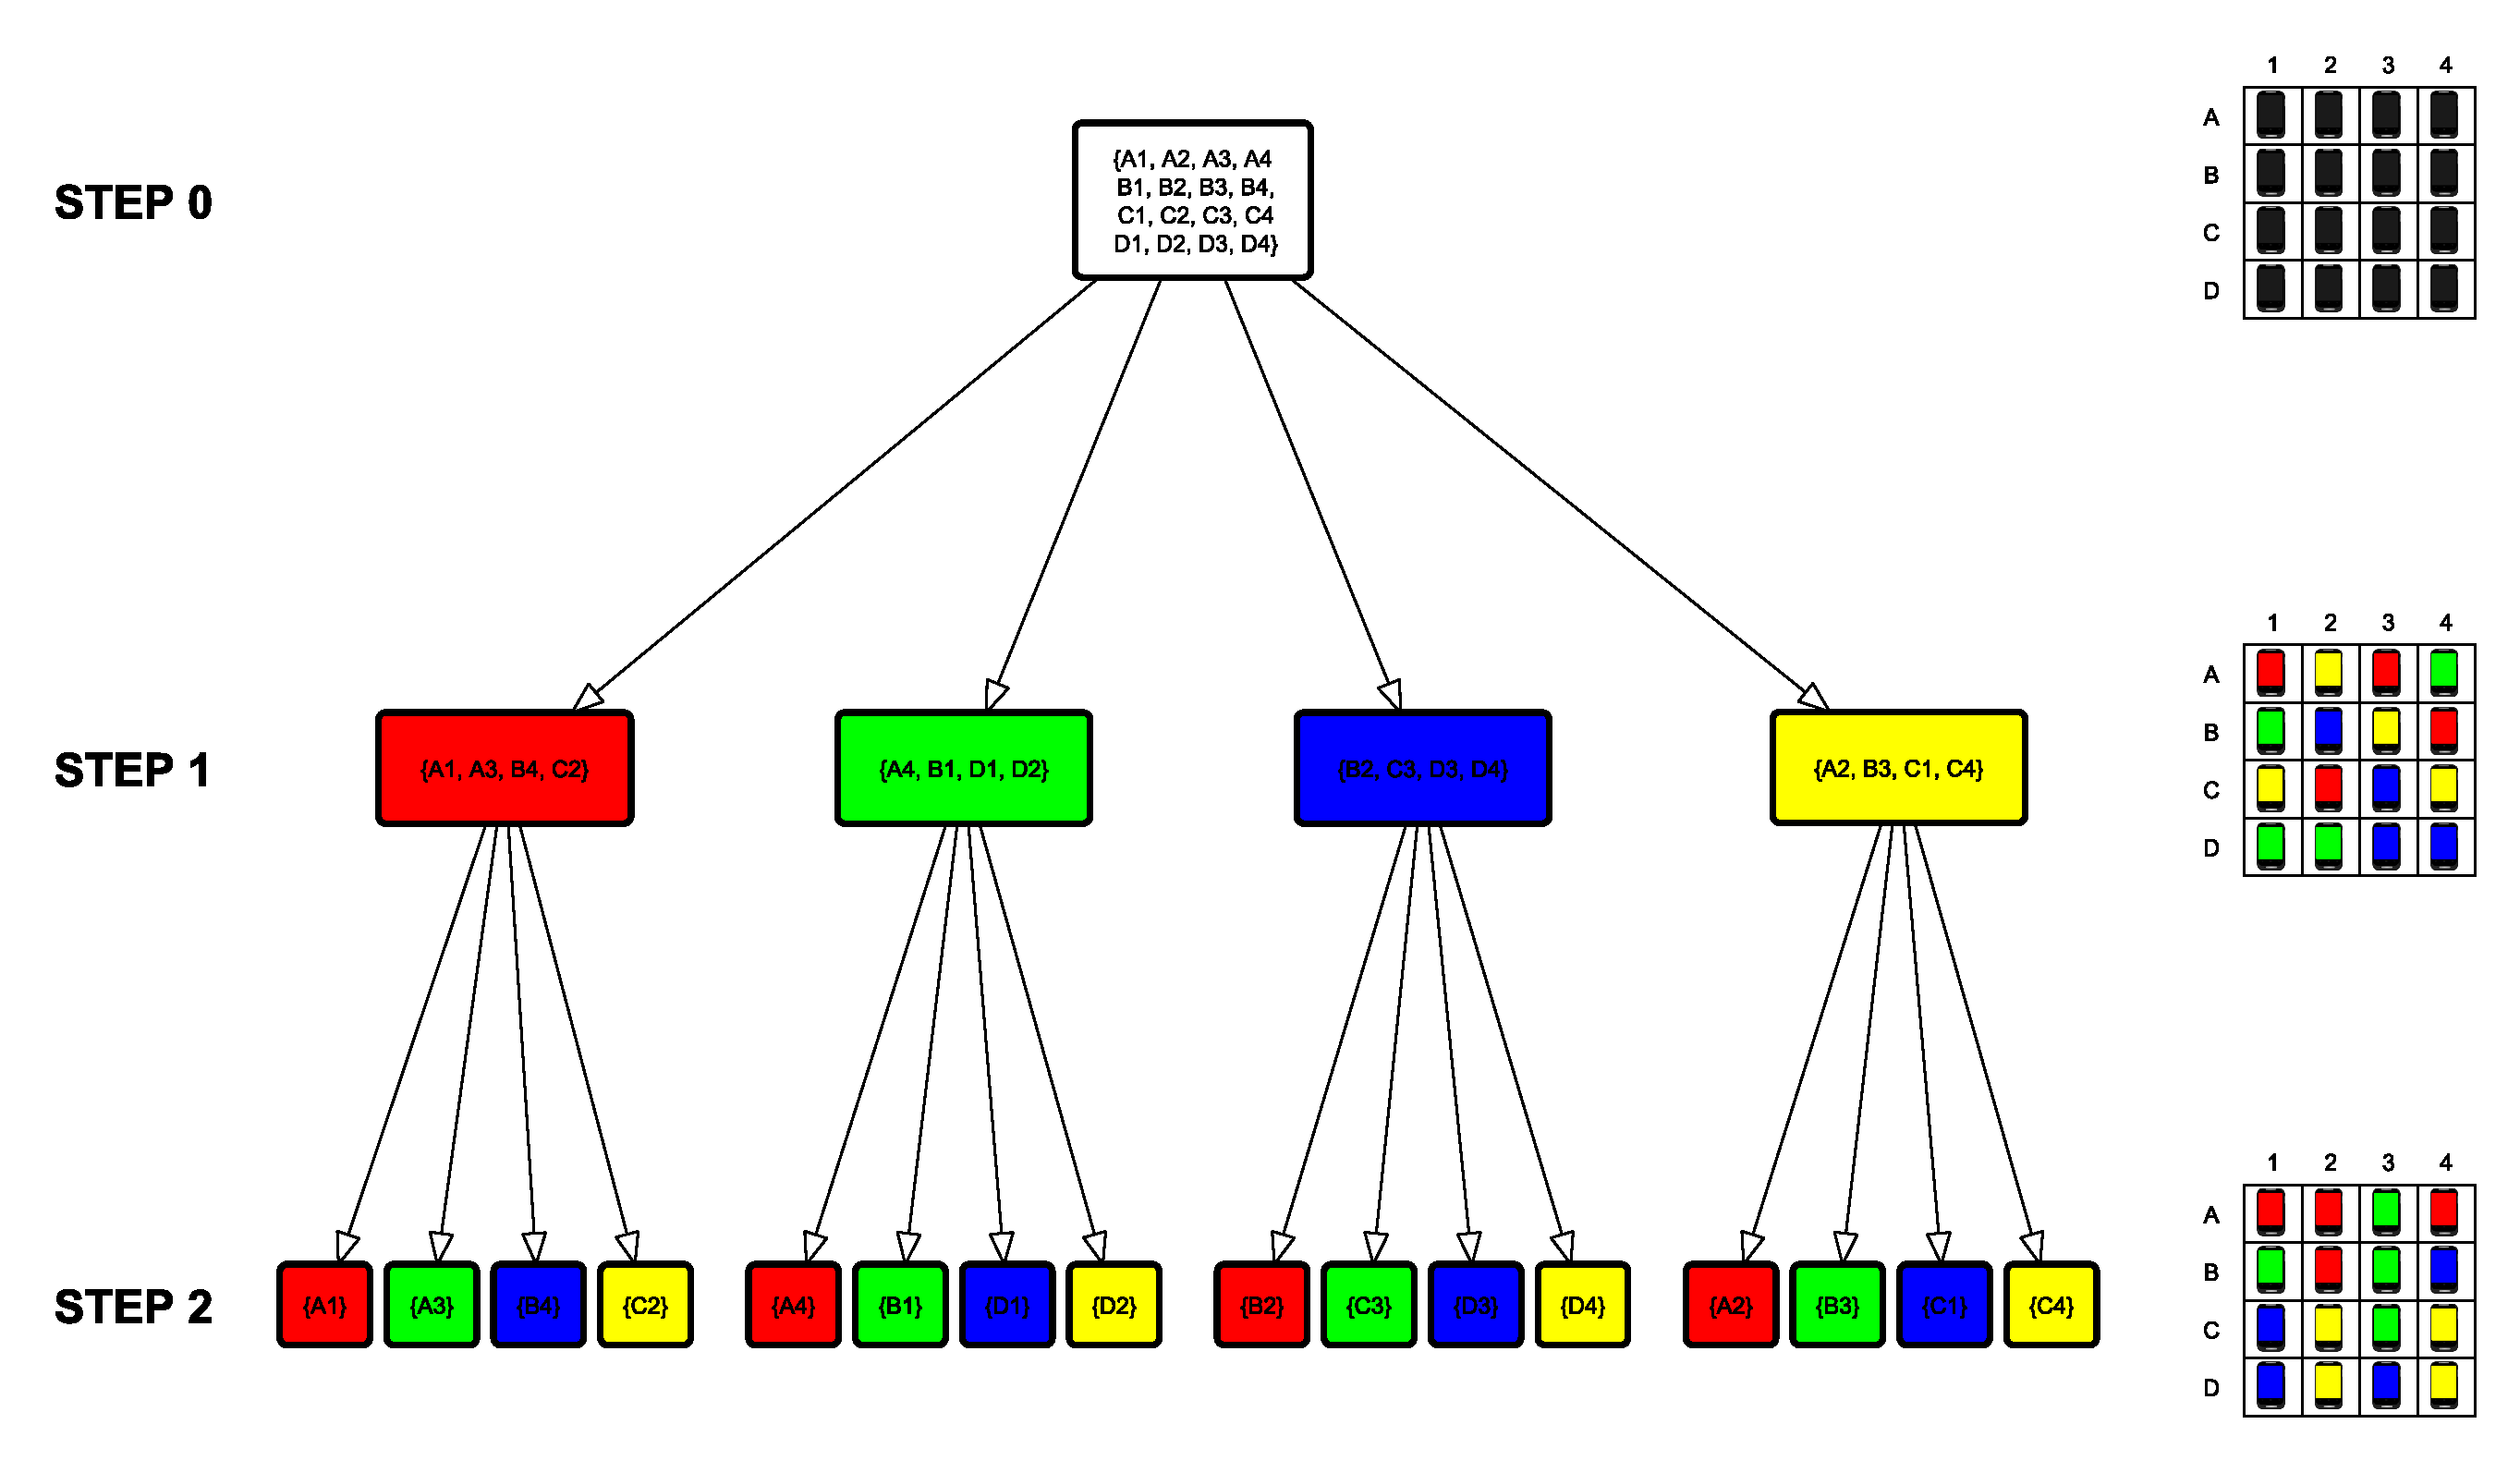
\includegraphics[width=18cm, angle=90]{sprint5/tree_algorithm.eps}
	\caption[Tree algorithm detection example]{Tree algorithm detection example. There are sixteen devices and four detected colors which means it is possible to recognize the position of all devices within two steps.}
	\label{fig:sprint5_tree_alg}
\end{figure}

\subsection{Limitations}
The main drawback of this algorithm is the position resolution. It is only be capable of distinguishing between all devices if there are no more than one device in each tile. Otherwise the ambiguities occur and the algorithm finishes in the state where some devices are assigned more then one possible positions.

Nevertheless it has been decided to disregard this issue as this project only serves the purpose of proof of concept and if needed these minor limitations might be improved on performing additional techniques that would solve the problem.

\subsection{Modification}
It might happen that certain devices are not recognized using this algorithm. Therefore this algorithm is accompanied by the former "one-by-one" approach. This fallback option is only invoked if there happen to be devices that failed to being recognized.

\subsection{Performance}
Given the divide and conquer base of this algorithm the time complexity is logarithmic, $T(n) = O(\log n)$, as compared to linear time complexity of the former algorithm. This is though the best-case scenario where all the devices are correctly recognized. In the worst case scenario where no device is recognized during performing tree algorithm the time complexity would be $T(n) = O(\log n + n)$.

\begin{figure}[H]
	\centering
		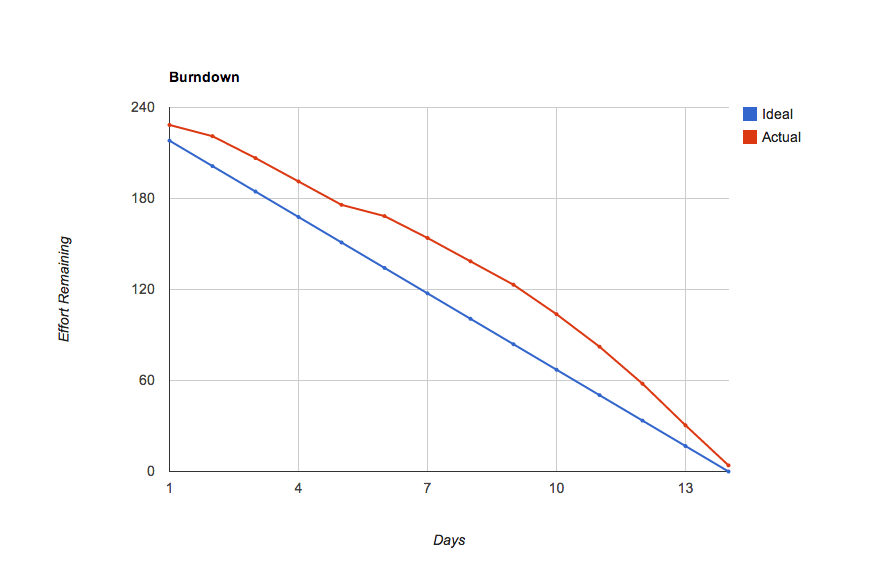
\includegraphics[width=18cm]{sprint5/BurndownSprint5.png}
	\caption{Burn down chart.}
	\label{fig:Burn5 }
\end{figure}

\section{Testing}
\section{Occurring risks}
\label{sec:sprint5_occuring_risks}
First time during development process, team have encountered the risk that might influence successful finish of the project. 
Restarting of client devices during runtime is noted. This issue didn't happen very often in the past, and source of it have been attached to not very stable Android device in team possession. Team were unable to replicate this error on other devices, and recklessly marked it as a isolated case. As number of testing devices become bigger multiple phones started to behave the same and it was obvious that it is not isolated problem. 

Researching Internet for similar problems lead to the
reason of client restarting - race condition inside \texttt{NsdManager} class. The issue is registered on the Android issues list\footnote{\url{https://code.google.com/p/android/issues/detail?id=35585}} and has been fixed on Oct 18. 2013. Release is planned for Android 4.4 so only changing Android NSD for some of the previous technologies can solve the problem. 

At that time, working on next core module (image processing), with knowledge that issue will be gone with next release of Android system, was preferable by the customer. For that reason team exchanged few e-mails with the customer explaining that previous decision to stick to Android NSD have multiple bad effects on the recording of final prototype:
\begin{itemize}
\item Team will be in possession of big number of Android devices for a limited period of time. If clients restart in middle of the presentation that will take away notably amounts of time.

\item NSD works just on devices powered by Jelly Bean(4.1.x) or KitKat(4.4). Most of the phones team have plan to borrow are not brand new and do not support Android NSD service.
\end{itemize}

Finally the customer agreed on adding another user story with high priority - Replace NSD communication module with one of the technologies previously researched.

\section{Customer feedback}
\section{Retrospective}
This section reflects on the past sprint. In order to learn from the mistakes done and thus to improve the workflow it is necessary to answer two essential questions: "What went well" and "What could be improved".

\subsection{What went well}
\subsection{What could be improved}


\chapter{Sprint 6}
\section{Sprint planning}
All implementation related stories for sprint 6 are presented in table \ref{tab:sprint6stories}.
%\caption{User stories selected for Sprint 4.}
  \label{tab:sprint4stories}
 \def\arraystretch{1.25}
 
\begin{longtable}{ccXcc}

\toprule[0.5mm]
\multirow{2}{*}{\textbf{ID}} &
\multirow{2}{*}{\textbf{Ref.}} & \multirow{2}{*}{\textbf{Description}} & \multicolumn{2}{c}{\textbf{Hours}} \\
 					& & & \textbf{Est.} & \textbf{Sp.} \\
%\textbf{ID} 	& \textbf{Description} 	& \textbf{Est.} & \textbf{Sp.} \\
\midrule
\textbf{I4.1} 	& 	& {\bf As a server I need to link the devices' location with their ids.}	 &  52	& \textbf{48} \\

\textbf{I4.2} 	& 	& {\bf As a server I need to identifiy multiple clients from light.}		 &  19	& \textbf{18} \\

\textbf{I4.3} 	& 	& {\bf As a server I need to map all available devices to grid.} 			 & 22 & \textbf{18} \\	

\textbf{I4.4} 	& 	& {\bf As a server I need to play the whole media to the grid.} 			 & 37 & \textbf{34} \\
	
\midrule
		
				&& \textbf{SUM:}		&		130	& \textbf{136}
 \\																			
\bottomrule[0.5mm]
\end{longtable}


All the documentation related stories for sprint 6 are presented in table \ref{tab:sprint6Documentationstories}.
%\caption{User stories selected for Sprint 2.}
\def\arraystretch{1.25}
 
\begin{longtable}{ccXcc}
\label{tab:sprint2Documentationstories}\\[-6mm]
\caption{Documentation stories selected for sprint 2}\\[-4mm]
\toprule[0.5mm]
\multirow{2}{*}{\textbf{ID}} &
\multirow{2}{*}{\textbf{Ref.}} & \multirow{2}{*}{\textbf{Description}} & \multicolumn{2}{c}{\textbf{Hours}} \\
 					& & & \textbf{Est.} & \textbf{Sp.} \\
%\textbf{ID} 	& \textbf{Description} 	& \textbf{Est.} & \textbf{Sp.} \\
\midrule


\textbf{D2.1} 	& 
	\refwbs{wbs_documentation}{WBS 8.2}	& {\bf As a student I need to finish the pre-study chapter.} 									& 	12	& \textbf{ 16} \\

\textbf{D2.2} 	& 
	\refwbs{wbs_documentation}{WBS 8.2}	& {\bf As a student I need to finish the planning chapter.} 									& 	10	& \textbf{ 14} \\

\textbf{D2.3} 	&
	\refwbs{wbs_documentation}{WBS 8.2} 	& {\bf As a student I need to finish requirements chapter.} 									& 	30	& \textbf{ 26} \\

\textbf{D2.4} 	& 
	\refwbs{wbs_documentation}{WBS 8.2}  & {\bf As a student I need to finish the architecture chapter.} 								& 	24	& \textbf{ 12} \\

\textbf{D2.5} 	& 
	\refwbs{wbs_documentation}{WBS 8.2}	& {\bf As a student I need to finish sprint 1 chapter.} 										& 	12	& \textbf{ 16} \\

\textbf{D2.6} 	& 
	\refwbs{wbs_documentation}{WBS 8.2}	& {\bf As a student I need to work on the  sprint 2 chapter.} 									& 	16	& \textbf{ 18} \\
%ASK group about this:
%\textbf{360} 	& \refreq{}
%	& {\bf As a student I need to start on the architechture chapter.} 								& 	?	& \textbf{ ?} \\	

								
\hline
				&& \textbf{SUM:}		&		104	& \textbf{102}
 \\																			
\bottomrule[0.5mm]
\end{longtable}


All the project management related stories for sprint 6 are presented in table \ref{tab:sprint6storiesProcess}.
%\caption{User stories selected for Sprint 1.}
\label{tab:sprint1storiesProcess}
\def\arraystretch{1.25}
 
\begin{longtable}{ccXcc}

\toprule[0.5mm]
\multirow{2}{*}{\textbf{ID}} &
\multirow{2}{*}{\textbf{Ref.}} & \multirow{2}{*}{\textbf{Description}} & \multicolumn{2}{c}{\textbf{Hours}} \\
 					& & & \textbf{Est.} & \textbf{Sp.} \\
%\textbf{ID} 	& \textbf{Description} 									& \textbf{Est.} & \textbf{Sp.} \\
\midrule

% === Process ==========================
\textbf{326} 	& 
	& {\bf  As a student I have to track effort time} 	& 		16	& \textbf{16} \\
\textbf{345} 	& 
	& {\bf As a student I have attend the weekly meetings with the customer} 	
	& 	22	
	& \textbf{?} \\
		&& Preparation for demonstration	& 2 & ? \\
		&& Demonstration	& 6 & ? \\
		&& Writing minutes 	&  6 & ? \\	
		&& Customer meeting	&  6 & ? \\
		&& Writting minutes	&  2 & ? \\
		
\textbf{327} 	& 
	& {\bf As a student I have to attend the weekly meetings with the supervisor} 	
	& 	12	
	& \textbf{?} \\
		&& Meeting in week I	& 4 & ? \\
		&& Meeting in week II	& 4 & ? \\
		&& Writing minutes from week I 	&  2 & ? \\
		&& Writing minutes from week II	&  2 & ? \\	

\textbf{344} 	&& {\bf As a student I need to attend the team building.} 	& 		7	& \textbf{9} \\
		

\textbf{321} 	&& {\bf As a student I need to participate to lectures about team dynamics. } 	& 		32	& \textbf{25} \\
				&& Course of group dynamics Thu.	&  &  \\
				&& Summary of course and exchange learned.	&  &  \\				
				
\hline
				&& \textbf{SUM:}		&		164	& \textbf{?}
 \\																			
\bottomrule[0.5mm]
\end{longtable}

\section{System Burndown}
\section{Architecture}
\section{Implementation}
\section{Testing}
\section{Occurring risks}
\section{Customer feedback}
\section{Retrospective}
This section reflects on the past sprint. In order to learn from the mistakes done and thus to improve the workflow it is necessary to answer two essential questions: "What went well" and "What could be improved".

\subsection{What went well}
\subsection{What could be improved}


\chapter{Testing}

\section{Types}
\section{Unit testing}
\section{Integration}
\section{System testing}
\section{Usability}
\section{Acceptance}







\chapter{Evaluation}
In this chapter the team will evaluate different aspects of the projects. 
Everything from team collaboration, the project assignment, the cooperation with both customer and supervisor, to risks- and role assignments. There will also be discussed how the team tackled challenges during the project, and how the team handled the project management. Briefly explained the team will discuss why and how the outcome ended up being what it is today.
This chapter is split into three major parts, which is group evaluation, project evaluation and technology evaluation. 

%_______________________________________________________________________________
\section{Group evaluation}
In this section the team will elaborate on how the group functioned as a whole, and how the team collaborated. The team will also evaluate both the customer and the supervisor, before moving on to the evaluation of the goals the team sat at the beginning of this project. After this the team will evaluate the challenges met during this project and how this affected the work. At last the risk and role assignment will be evaluated.

\subsection{Team dynamics}
In this section is about how the group functioned as a whole, how the team communicated, the work distribution, and at last our motivation.

\paragraph{In general}
The group was randomly put together, and the number of people in this group was four.
Each person with different personalities and interests. A perfect atmosphere was not expected. Fortunately the team had no major conflicts, only constructive discussions. For the most part the team functioned well together, and offered each other help when needed. 
Overall the team feels like the team work, and progression of the project was good.

\paragraph{Communication}
Good communication within a team is important. For a team to perform it needs a safe and stable working environment. The importance of this was addressed early on. 
It was decided that every decision made in the group should be a result of a democratic process, which meant making decision by the majority vote. 

The communication was mostly done collocated. Mostly because of our agreement of sitting in the same work area as much as possible. This turned out to be a good rule most of the time. 
When every one was siting together it was never difficult to get help from the rest of the group. This enabled the tea, to quickly discuss points in doubt, and continuing with the work. This also gave the team a smoother work flow, a quicker progression, and it gave the team more time to revise and improve the work.

Because of completely different schedules, it was not always possible to sit collocated. Often there was a team member missing at working hours. There were a few situations where the team would have benefited from having the entire group present, but there was nothing the team could have done. Luckily it did not affect the project too much. The team solved the problem by using Facebook. If someone had other obligations, and they were not able to be present, then the team kept in contact through Facebook. This was a suitable solution since the team members were available online often. This made coordination an easier task, since all of the team members could respond as soon as possible. 

There were a few problems with the groups communication. The team were too much dependent on the team member responsible for the communication. The team did not always get copies of emails written to the supervisor or the customer. This caused a little confusions regarding the meeting hours from time to time. It was also the cause of important information coming a bit late. The team should have had more strict rules for this.

In hindsight the team is able to point out a couple of things that could have made the communication better. The team could have done more stand ups. The lack of stand ups was another problem caused by the different schedules. The team tried to solve this problem by having longer meetings when needed, or suggested by a team member. Still, the team should have had more clear rules about stand ups, and this could have made the communication easier. 
More communication with other groups taking this course was another idea that could have improved the team communication.
Although the tasks were different, the exchanging of ideas and sharing experiences on both group dynamics and processes could have affected the team in a positive way. 

The team also had some social gatherings to get to know each other better, and throughout the project the team got well known with each other. This made the communication easier for us as a team. By learning from each other, and learning to put aside differences, one can say that everyone has grown as individuals. In spite of a couple of bumps in the road, the team feel that the issue of communication was handled pretty well.

\paragraph{Work distribution}
The distribution of work was challenging at times. 
The team had little experience with image processing, and therefore it was hard to be sure about the exact work load. Naturally this also made it difficult to maintain a balanced workload throughout the project. 
In the beginning the team agreed on what needed to be done, and then group members had to take individual responsibility to perform work on the tasks they were comfortable with. 
Towards the ending of the project it was a bit stressful, because of troubles with the final demonstration video. Suddenly the team needed to spend more hours than expected. This is something the team should have anticipated, and the team should distributed the work a better.

\paragraph{Motivation}
All team members were very motivated. Everyone wanted to receive a good grade in this course, since the course was very relevant for us.In this course the team had to use knowledge from several different courses in previous years. Another motivation was the project assignment. The fact that the assignment was interesting increased our motivation and efforts. It was exciting and the team had the opportunity to learn something new. Our customer was also a great motivator, and by forcing us to deliver something at the end of each sprint, the team always felt like the milestones was reached. This way we always felt one step closer at the end of each sprint, and it became very motivating to continue the hard work. 

\subsection{Customer and project task} 
Our customer, Peder Kongelf, was pleased with the results. During the last customer meeting he informed the team that the project goal was reached, which was to make the audience as a screen at a rock concert, and to do this using image processing.
This project was a proof-of-concept project, and if someone wanted to do further work on our application the only remaining parts would be performance and scalability. 
The team wanted to have a bigger "wow-effect" on the last video demonstration, but we did not have enough resources to conduct this. With the demonstration video it is only possible to see the potential the project has. All in all the customer was satisfied with this result. 

The team is very impressed with our customer. The project given to us for this course was extremely exciting. The team got to work with challenging and new technology, which was really great. The fact that the task was interesting increased our motivation and efforts. He had plenty of experience with working as an consultant, and he was eager to teach us as much as possible. The team also wanted to learn as much as possible from him. He gave us good advice through out the whole project. One of the best advices he gave was about working together as much as possible. Looking back the team realizes that otherwise communication challenges could have been much tougher. Our customer also helped us with the scrum methodology. He taught the team a lot about everything from epics, user stories, task, estimation, to reviews. All of this was extremely useful for the team.

Early on Peder suggested weakly meetings, which was good. He always gave the team great feedback, as well as giving an impression of having confidence in the team. Sometimes, because he had a great amount of work load him selves, the meetings where shortened. Still, he was involved and enthusiastic about the project. Of course the team expected some communication problems from time to time. This was challenges like confusion over meeting hours, but the team addressed these issues very smoothly. The final conclusion about the customer is that the team would not have been able to deliver this end result if not for the great effort and constant feedback from the customer. 

\subsection{Supervisor}
Almost every week the group met up with the supervisor. In these meetings the progress made by the group was presented, and the supervisors came with feedback on the report and other work. It was quite useful to know whether the team needed to increase the work speed or not. 
The supervisors also gave feedback on the content of our report, which was useful for the team.

Before the meetings the team sent out a meeting invitation to the supervisor.
If there were something in particular the team had questions about, then the relevant documentation was emailed to the supervisor before the meeting, so the he could get a chance to look at it before the meeting.

In the beginning the meetings were useful in order to assure that the team were on the right track. After a while there was less need for a weekly meeting, because the team had a better understanding of what the report should look like.
Maybe a shorter meeting would have been more sufficient for the middle part of the project 

The communication with the supervisor could have been better time to time. Especially there was a little misunderstanding when the supervisor had to travel to a conference, and some of the team members showed up to a canceled meeting. This was just little bumps in the road, and most of the time the supervisor was available, and gave us really valuable feedback, especially with the report. 

\subsection{Goals} 
In this section the team will evaluate the project goals, the group goals, and our personal goals, to see if the team achieved them. 

\subsubsection{Project goals}
\paragraph{Finish the project within the scheduled timetable}
The team finished the project within scheduled timetable. It was a little stressful towards the ending, but this goal was reached.
\paragraph{Finish the project with the specified requirements}
The project was finished with the specified requirements, and the team made a demonstration video for the final presentation to show off the system. This goal the team achieved. 

\subsubsection{Group goals}
\paragraph{Receive a good grade or a good recommendation}
At this stage it is difficult to determine whether this goal was achieved or not. Looking back at setting these goals the team realizes that setting more measurable goal would have been better. The team has learned from this, and will take this experience with us fore future projects.

\subsubsection{Personal goals}

\paragraph{Agnethe}
One of my personal goals was to learn more about group dynamics and collaboration. This I have definitely done. Working as a team can be challenging at times, and I have learned a lot from this experience. Another goal of mine was to learn more about writing reports. Writing this huge report has thought me a lot about technical writing, and I feel more prepared for writing reports in other courses later on. A goal that is hard to determine at this point is whether im better at holding presentations since this report is supposed to be finished before holding the final presentation. The last goal I would like to mention is that when I wrote the goals in the beginning of this course I wrote that  there is a great chance that I would work as an IT- consultant. Looking back at this and I realize that I really enjoyed this experience. Working as an IT-consultant is something I would like for the future. 

\paragraph{Jan}
When looking back on the whole project timespan now I see that one of the main purpose of this course was to teach students to cooperate and communicate both together in development team and also with the other project related authorities such as the supervisor and the customer. I gained the idea of what does it take to work under agile methodology Scrum and I appreciate this experience as I might come across it in my future carrier. I also improved my skills as far as the Java/Android programming is concerned but not as much as I expected mostly due to the fast tempo and the need of doing other tasks. Even thought sometimes boring I appreciate that writing technical documentation was a part of this project as I definitely improved my English writing skills. As for the course itself I must admit I was a bit disappointed by the organization and the lack of lectures and/or other sources of information related to the project. I enjoyed working with my team colleagues though and to conclude I feel this course was beneficial for me.

\paragraph{Milos}
After 13 weeks of team work my primary goals and expectations from this course have been fulfilled. I learned how to be part of the team and how to collaborate with other people in achieving common goals. Further more I was enjoying working with new teammates. Overall atmosphere was great, team spirit was on high level and we even spent time together beside this project. For this reason, we were able to finish all of the set requirements and manage occurred risks and minor conflicts without big effort. Writing documentation helped me with technical English, just as expected, and practicing SCRUM gave me a picture of how real companies manage their development cycle. For me this project was absolute success and I will be proud to add it to my CV.

\paragraph{Tomas}
During this course, I have enormously improved my written English. 
It was also useful to learn about technical writing in English language, since some of the rules are different than in Czech.
Working in group and collaboration was sometimes difficult, due to different views of team members, and there is often need of compromises.
I have increased my knowledge in topic of architecture and software design and I have learned a lot of new diagrams.
Unfortunately due to the work distribution, my Android platform development skills have not improved as I expected, because other more knowledgeable team members were responsible for these parts.

\subsection{Challenges}
The team will in this section reflect on the challenges experienced, why they occurred, and what we could have done differently.

\paragraph{Time and time estimation}

Throughout the project, time restrictions has been a challenge because most of the members in the group have had other projects during the semester. Agnethe had two different projects in addition to the customer driven project. Milos also had another project that was quite time consuming in the beginning. Jan and Tomas also had another projects besides the customer driven project, and Jan also wanted to take Norwegian classes. All of this made it hard to find suitable working hours, and time. 

The actual amount of logged work fell a little short of the expected amount of hours. Still, the team were able to successfully execute the tasks  planned. The team also feels like the shortage of hours did not have any significant detrimental effect to the project. 

Regarding the time estimation, the team thinks the estimates were within reasonable bounds, but still it could have been better estimations for some of the user stories. To improve these time estimation the team could have done a better job using the planning poker. While reviewing this the team realizes that realistic time estimation is valuable, and that this project has taught us a lot about this.

\paragraph{Language and Cultural Barriers}

Within the team there were three different nationalities. The were one Norwegian, one Serbian and two Czechs. Since there were different nationalities the communication had to be done in English. English was spoken internally in the group. The communication with both the supervisor and the customer
was also done in English. It was a challenge to have all communication in English. Solutions and technical issues is probably easier to discuss in a persons native language. This caused challenges during the decision makings. It was spend more hours then expected discussing some issues, because it was hard to express everything in English. It was also hard to get a clear understanding of the different arguments. Sometimes Jan and Tomas switched to Czech, to be able to help each other. Sometimes it was easy to lose focus during discussions when the language was switched, but most of the time it was very useful and it progressed the discussion.

Since everyone was used to study at different universities, with different cultures, and with different ways of doing things. The team sometimes had different methods for solving problems. If the team could not reach a decision, it was decided to ask the supervisor or customer to get additional information, and then try to make a new decision. Very often this helped to shed new light on the situation. If the team still could not make a decision the majority vote was used. For the most of the time language and cultural differences was not a problem. Everyone was excited to learn, and teach each other. 

\subsection{Role assignment}
As mentioned earlier the role assignment were adapted a bit, so they could fit the project better. Also the roles assigned to each group member was more of a guideline, rather than a binding responsibility. This was mainly because for some of the team members, this was their first scrum project. Some of the roles required more experience and knowledge then the group member had. The team solved this problem by working together, and helping each other. 

Looking back at the role assignment it is not possible to deny that there are things that could have been differently. Since everyone was working with mostly unfamiliar technologies in the beginning, it might have been a good idea to make each of the role's responsibility more clear, and enforcing them in the early stages of the project. Also, the team could have have spent more time researching the roles actually needed. Even though it was decided to embrace this as an equal development team, the roles might have been useful for us it these improvements had been done. 

These are the roles assigned, and this is how they were evaluated.

\paragraph{Project Leader}
The project leader was supposed to be responsible for the project progression, and delegate tasks to the other team members. This did not work very well, because the tasks was prioritized by the customer. If one task was done, the team member had picked the task with the highest priority to do next. All of the team members took responsibility for the progression of the project, and tried to make sure that it went according to plan. The description of this role also claimed that the Project Leader had final call in arguments. This was not the case, since it was decided from the beginning that this as an equal development team.

\paragraph{System Architect}
The system architect was responsible for checking and analyzing all the layers in the product, but this was also something not only one person took responsibility for. 

\paragraph{Scrum Master}
The Scrum Master role was assigned to one person originally. Nevertheless, all team members took responsibility for following up on this. It became natural to suggest to have stand ups during working hours, since it was not always easy too keep track of what the other team members were working on. Having the whole team responsible for scrum methodology worked for this project, because of the team members having different schedules. 

\paragraph{Communication Responsible}
This is the only role that was used throughout the whole project. The reason for this is because it was easier for the team to keep track, and it was also easier for both the customer and supervisor to have only one person to communicate with.    

\paragraph{QA Responsible}
The QA was responsible for the quality of all documents and the end product. Still, the whole team felt responsible for delivering a product with good quality. The QA was also supposed to help determining if stories and acceptance criteria was well defined. For this project it was difficult because it was hard to do with little experience. A QA is also responsible for organizing testing, and this includes that unit tests are well written, provide developers with high level test cases for the stories, and performing exploratory testing on early builds. For this project the testing part was not a priority. All of the above resulted in that this role was not used.

\paragraph{Documentation Responsible}
This is a role that all team members took responsibility for. It was smart having one person responsible for setting up a good structure in the beginning. After a while everyone participated where they could. 

\subsection{Risk evaluation}
In this section the risks from the risk Table \ref{tab:risks} in the planning section, will be evaluated. Among these risks the team only experienced a few of them.

\paragraph{Sickness/Absence}
Some of the team members where exchange students, and they wanted to travel and experience Norway during the semester. Naturally it lead to some absence at times. When this happened the team members worked extra hard for this not to affect the project. This was also the solution if members got sick, and for this project this was a good solution. 

\paragraph{Coding problems}
To some extent the team experienced some coding problems, but the team figured it out. At the end it was possible for us to reach the project goals. This is a risk that probably occurs in most projects. Because of reflecting over the risks the team was prepared that might happen.

\paragraph{Testing problems}
This risk did not occur, since the customer told us not to focus on the testing part.

\paragraph{Changing requirements} 
The team did not experience problems with requirements changing too much. The communication with the customer was really good, and possibly because of the reflection over this risk, the problem was avoided.

\paragraph{Dead end with technologies}
While doing research for existing solutions the team experienced difficulties. The team could not find a good existing solution. Luckily the team found OpenCV, and by using this it was possible to finish the project. 

\paragraph{Unrealistic time estimation}
It was not easy to estimate all of the user stories. Sometimes the team underestimated and other times the team overestimated. Towards the ending of the project it was a bit stressful, but mostly this did not affect this project.

\paragraph{Customer too ambitious}
The team did not experience that the customer was too ambitious. The reason for this was because the communication with the customer through out the project was very good. The team and the customer had good sprint reviews, and planned the next sprint together.

\paragraph{Hardware problems}
The team had some hardware problems. For this project the team were dependent on borrowing phones to be able to test the system. It was not easy to borrow phones from a lager amount of friends at the same time. The hardware problem was that the team did not have enough resources. Luckily the team was able to borrow phones two times. The first time the team experienced some troubles with the school network. Phones connecting to different subnets at NTNU made it difficult test. To solve this problem we needed our own router. The problem was solved by shooting the final demo-video at one of the team members apartment. If this risk had been more concrete from the beginning, the team could might have foreseen this.  

%_______________________________________________________________________________
\section{Project Evaluation}
This section will start with an evaluation of the preliminary studies, and the planning phase of this project.  
Then the team will evaluate the utilization of the scrum methodology, before moving on to a summary of the meetings minutes. 

\subsection{Preliminary Studies}
In this section the team will evaluate the preliminary studies done for this project.
\paragraph{Similar projects} 
The team is satisfied with the fact that similar projects was researched, because it gave inspiration for which effects the Digital Lighter should be able to play. 

\paragraph{Software development methodology}
The research of the methodologies was time well spent, because it helped the team to learn more about Scrum, and how to carry it out in practice.

\paragraph{Development technologies}
This research was the most important one. It was also what the team learned the most from. Looking back the team realizes that spending even more time researching could have been helpful, but with the given time frame this would be a too big of a risk.

\paragraph{Project management tools}
The team became better acquainted with the Scrum while spending time finding a suitable project management tool. Too understand what kind of features this kind of tool needed, the team gained a better understanding of Scrum, which was positive. What was negative was that the free tools were definitely not perfect, and the team spent more time then necessary trying to choose between several incomplete tools. 

\paragraph{Documentation tools}
Researching documentation tools gave the team an opportunity to learn more about LateX, which was planned to use for writing the report. This was very helpful since not all team members had experience using it. 

\subsection{Planning}

It was useful to plan the project, because the team got more aware of the strengths and weaknesses within the team. Therefore the time spent planning the project was not wasted. It also helped the team working more goal-oriented. In the beginning of the project the sprints was planned together with the customer. This was valuable for us, because the team avoided confusion regarding the requirements. The team also learned a lot about estimation of user stories. Doing the planning by our selves later on, this knowledge became very useful. Reviewing the time spent on planning, there is no point denying that the team could have planned the sprints better. This might have helped with avoiding stress towards the end.   

\subsection{Scrum}
The scrum development methodology was chosen early on even though some of the team members were not too familiar with it.
Still there were many good reasons why the team chose to utilize Scrum.
One of the reasons was the risk of sudden changes in the requirements.
Another was that it would be easier to monitor the progress. Staring the implementation early was also a good argument. Also the fact that the team would most likely be using agile methods in future projects. 
This was also the methodology the customer wanted us to use. 

Using Scrum was difficult at first as only some of us had any previous experience. 
In addition, the project scope was not properly set at the beginning, which made building the product backlog difficult. 
The team did not follow the Scrum convention for user stories as an example. 
All of the stories had to be changed later on to make them more consistent. 
The backlog also contained stories for writing the report and attending meetings.
The team decided to add this to report anyways, because it showed very clearly how the had carried out the project from the start till the end. 

Even though the team tried to adapt scrum to the project, one of the negative experiences was the stand ups. As a student there are several courses to take into account, and this made daily stand ups difficult to follow through. Therefore Scrum could have worked better if the team worked more as a unit with more strict working hours from the beginning.

The positive experience was that the concepts of sprints. Everything from planning to  the retrospective was well conducted, and the team learned a lot. The team also held a demo presentation for both the customer and the advisor at the end of every sprint, and this helped with keeping them updated, and opened for some feedback. Based on this feedback it was possible make the necessary changes in time.

Even though the team have had some difficulties with Scrum, the team are glad for using this methodology. Scrum made it simple to implement changes in the project, and continuously produce results that could be discussed with the customer. It would have been challenging to complete the project with a waterfall methodology, because it was important to start the implementation early.  

In the end we were able to deliver a product that we and the customer was very happy with, which in hindsight can make us say that the team was right to choose Scrum.

\subsection{Meeting summary}
Looking back the team feels like the meetings were useful. It was essential to have a good communication with the customer, because it was important not to get sudden changes in the requirements. It was also important to be sure that the customer was satisfied with the product throughout the project. While writing this report the team realized the advantage of having good meeting minutes. It was useful to be able to go back and check thoughts on decisions and thoughts on the project in general, while writing.

In the Appendix it is possible to see an example of the meeting minutes. The customer meeting minutes is in Appendix \ref{chap:customer_meetings}, and the supervisor meeting minutes is in Appendix \ref{chap:supervisor_meetings}. 
%_______________________________________________________________________________
\subsection{Course feedback}
In this section there will be an evaluation of the Customer driven development course. The team will evaluate the lectures given in this course, and evaluate the course in general.
The course in general, the project task and the lectures will be evaluated.

\subsubsection{The lectures}
In this section the team will evaluate the different lectures that were held in this course.

\paragraph{Course in group dynamics}
This course focused on making the participants aware of that everyone is different, and handles things differently. Another important focus was the awareness of collaboration. The course made the team more aware of that working together will get us further. It also made the team aware that the other group members can help with reflection during a decision making. The course also forced us to discuss the groups different goals, and the different expectations. 

This course was one of the more useful lectures, since it improved the awareness of people's differences
and that their way of behaving is different, and that forced the team to discuss how to make decisions and solve conflicts if they occurred. To give some criticism, it can be mentioned that this course should have been earlier in the semester.

\paragraph{Presentation in agile software development and estimation techniques}
This lecture focused mainly on Scrum methodology, but it also compared agile software development to other methodologies. This lecture was helpful for the team because i was decided to work in Scrum. Since only one team member had used this methodology before, it was helpful for the team to learn more about the basics. 

\paragraph{Seminar in technical writing}
This lecture was useful since it gave the team a understanding of how a technical report should be written. The only critique is that some of the feedback the team got was not consistent with the feedback given by the supervisor.

\paragraph{Course in presentation technique}
This lecture was some what useful. The team got some tips on sales, and how to hold a good presentation. These tips will be taken into account when preparing for the final demonstration. 

\subsubsection{Final comments}

All in all this has proven to be a very valuable course. It has given the team a proper insight into the how's and why's of a software development process. Everything from the very start to the end of a project. The team have learned more about how to plan, estimate and research during a project. Also the team learned more about implementation and new technologies. Of course the team also gained some experiences with utilizing the scrum methodology, and working together as a team. 

It has been exciting to work with a real customer, and learning more about working as an consultant. This was huge motivation for the team, because the team really wanted to deliver something the customer would be pleased with. All in all this has been a successful project, which the team has learned a lot from.

%_______________________________________________________________________________
\section{Technologies and tools evaluation}
In this section you can read about main used technologies and tools during developing.
Emphasis is placed on problems encountered during using these tools and technologies.

\subsection{Android}
A brief description of Android operating system have been given in Section \ref{subsec:image_processing_library}. Building system under this platform had some advantages and disadvantages. Main points of both groups will be presented but bottom line goes in favor of positive points - Android OS was a good choice.

Disadvantages:
\begin{itemize}
\item Platform fragmentation - Right now, there are so many different devices out there, it is extremely difficult to put together an application that even runs on all of them.
\item Late support for multicast DNS-based discovery - For now only Android 4.1 adds support this feature, and that leave more than 30\% of the devices behind. Even working devices have issue described in Section \ref{sec:sprint5_occuring_risks}.
\item OpenCV library for Android is still relatively new and missing some of the original library features as described in Section \ref{subsec:openCV_reflection}.
\end{itemize}

Advantages:
\begin{itemize}
\item Good documentation - Android is very well documented and covered with training tutorials and lessons \footnote{http://developer.android.com/training/index.html}. This helped the team members who have not previously met with programming mobile applications. 

\item Large community - This means a lot of answered questions, and lot of developers ready to help you with problems. In some situations it was enough to check few forums, and developing problems will be solved.

\item Biggest part of the market share - Considering the survey carried on by the well established analyst, the company IDC, as of Q2 2013 Google's Android OS held almost 80 \% of the market share\footnote{\url{http://www.idc.com/getdoc.jsp?containerId=prUS24257413}}. This means that even with cut of 30\% because of platform fragmentation, team can target the biggest number of the devices. With changed networking module as described in Section \ref{sec:sprint5_occuring_risks} Digital Lighter Client application can be deployed on more than 95\% of the Android devices. This also means that team was able to easier collect sufficient number of devices for final demo video.

\item Big number of third party libraries - Popularity of platform made everyone porting all kind of libraries to Android. Team was using some of them during the development process like OpenCV, JmDNS and netlib\footnote{https://github.com/simmons/netlib}. 
\end{itemize}

\subsection{OpenCV} \label{subsec:openCV_reflection}

OpenCV is an open source computer vision library briefly described in Section \ref{subsec:image_processing_library}.
It is a very useful library, which saved the team a lot of time instead of implementing image processing parts themselves
 -- whole light detection module was just enhanced demonstration example of OpenCV functionality.

On the other hand, some problems with this library occurred.
OpenCV Java API is a relatively new and therefore some implementation is missing.
One example of this was described in Section \ref{sec:sprint3_implementation}.
This raised a lot of problems, which resulted into discarding of user story.

OpenCV Java API can be therefore counted as a immature product but with a high potential in future, provided OpenCV developers will focus more on this API.
At this moment, new release 2.4.7 if OpenCV is 44 days late according to the plan\footnote{\url{http://code.opencv.org/projects/opencv/roadmap}} with still 32 opened bugs or new features.

\subsection{Git}
The team adopted Git as its version control system since early phase as described in Section \ref{subsec:git}.
Most of the members had experience with some other VCS such as Subversion and therefore the idea of versioning was not new.
On the other hand, three of four members of the team had no experience with Git itself.

Even though Git is a powerful tool with a lot of features, the main reason of using was to share code.
Since development was rather linear, branching was used rarely.
On the other hand, support of releases was used quite often \footnote{\url{https://github.com/dohnto/DigitalLighter/releases}}.
This was very comfortable for creating a final report, when the team could easily see exactly what features were included in each prototype and also it was possible to se the GUI of product in particular phase.

Of course, troubles during merging occurred.
Since merging conflicts can be sometimes demanding and usually requires a deep knowledge about merging code, sometimes it was impossible for one person to solve it.
These conflicts were in most cases solved by discussion with all interested members.

After all the experience with Git is rather positive. 
It is always good to be able to work with tools, that a lot of companies use in real development.


\subsection{Target Process}
Target Process is a collaborative project management tool described in Section \ref{subsec:targetProcessToolDescription}.
This tool was chosen after two another tools were tried.
It is very complex tool for large teams and it provides many different views on project (called boards) and also offers to personalize these views.

This tool was used mainly for a collaboration with customer. 
Before sprint planning, user stories for next sprint were prepared and inserted into Target Process.
Customer could easily prioritize these stories by dragging and dropping.
He could also see spend hours on particular story and also the progress bar depicting progress of this story.

Sometimes, due to lack of a discipline, the spend hours and finished stories and tasks were not filled in time and therefore the retrospective cannot be that precise.
Anyway, Target Process was very mature and useful tool for customer communication with much more features that was for this project necessary.


\subsection{TestFlight}
TestFlight service, described in Section \ref{subsec:testflight}, was adopted because of customer proposal.
The service was used in early phases of development for customer comfort when testing the product.

Since the beginning of implementation, some non-reproducible errors occurred in client application.
After some testing, the team suspected TestFlight of those problems.
TestFlight for Android is relatively new service \footnote{\url{http://blog.testflightapp.com/post/49971420302/android}} and there it was decided to discard it from the implementation.
After some time, the team has discovered, that the issues were caused by Android system itself, as described in Section \ref{sec:sprint5_occuring_risks}, but the TestFlight was never used again, because the demonstration for customer were performed in form of videos.
 
Therefore it is difficult to evaluate tool, that has been used only for a short period of time.

\subsection{Technical issues}
During testing light detection module, problem situation\footnote{Tested with Samsumg Galaxy S3 and Samsung Galaxy S2.} with mobile devices camera was encountered.
In dark, if a tracked object (mobile phone lighting with single color) or camera itself is moving, everything is working as expected.
But if both object and camera are static, after some time, the camera starts to adjust the colors.
You can see that situation in Figure \ref{fig:screen_colors_in_enviroments}.
This is probably caused by exposure settings, and further research concerning that topic would have to be done.
\begin{figure}[h]
        \centering
        \begin{subfigure}[b]{0.4\textwidth}
                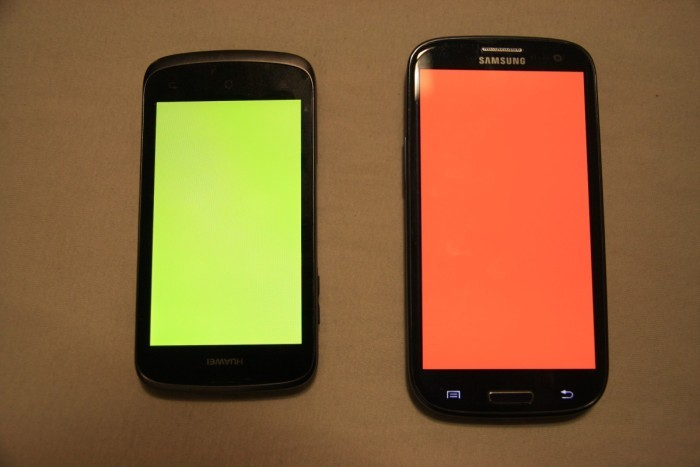
\includegraphics[width=\textwidth]{evaluation/IMG_7029.JPG}
                \caption{Colors of screens in light environment}
                \label{fig:tiger}
        \end{subfigure}
        ~ %add desired spacing between images, e. g. ~, \quad, \qquad etc.
          %(or a blank line to force the subfigure onto a new line)
        \begin{subfigure}[b]{0.4\textwidth}
                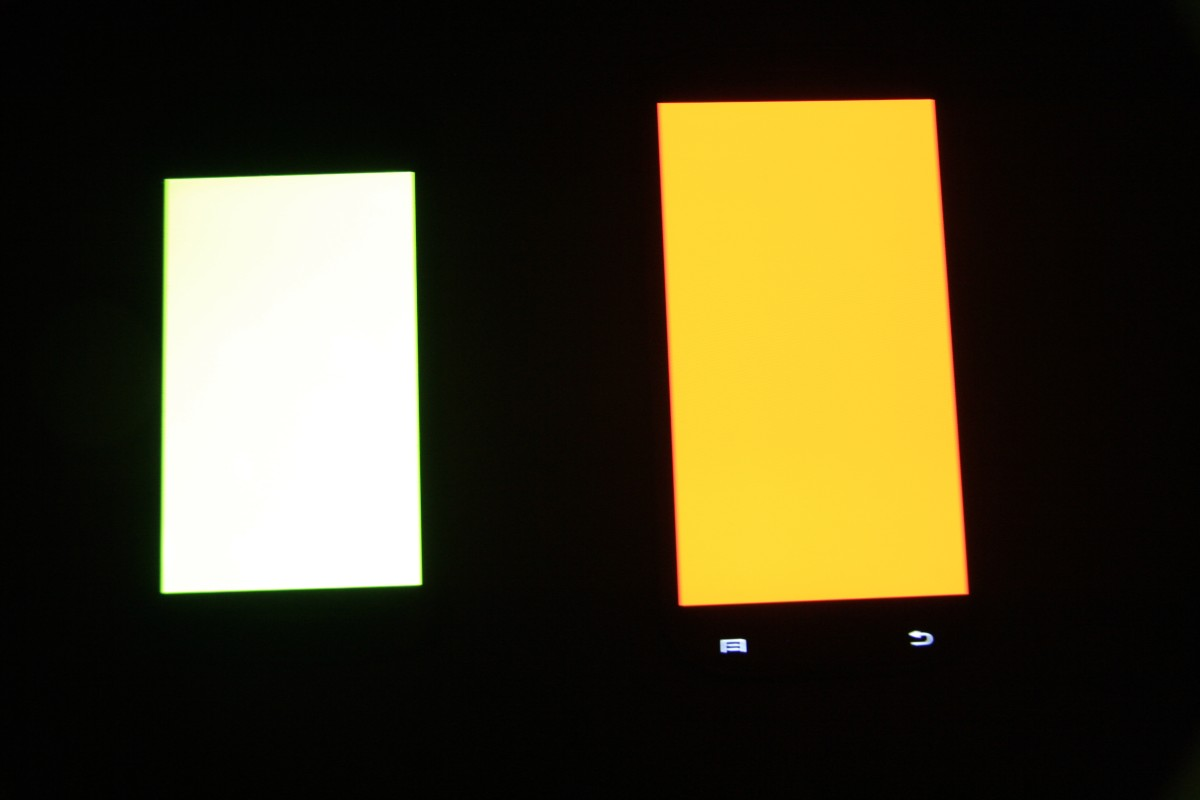
\includegraphics[width=\textwidth]{evaluation/IMG_7032.JPG}
                \caption{Colors of screens in dark environment}
                \label{fig:mouse}
        \end{subfigure}
        \caption{Colors of screens in different light environments}\label{fig:screen_colors_in_enviroments}
\end{figure}
By empirical research there were established colors (e. g. blue and white) which are least affected by this behavior.


\chapter{Conclusion}
\section{Introduction/Final product/description}
\section{Results}
\subsection{Server-side application}

Maybe we can present milestones reached

\begin{figure}[H]
	\centering
		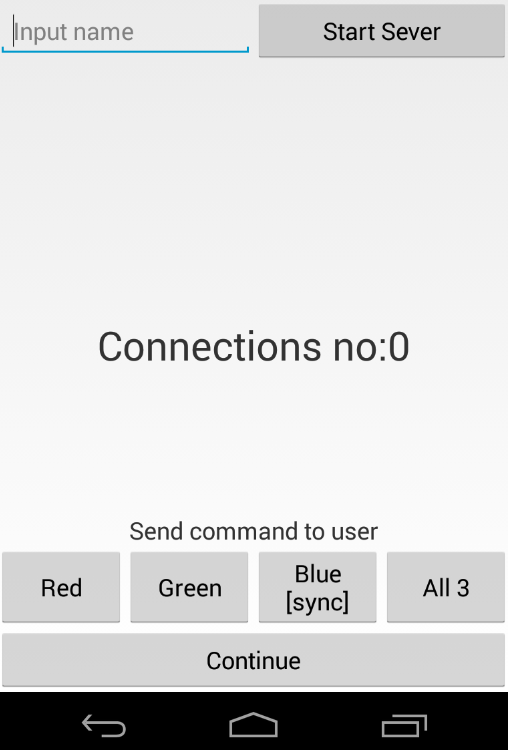
\includegraphics[width=5cm]{conclusion/server_ui.png}
	\caption{Server UI}
	\label{fig:Server_UI }
\end{figure}

\subsection{Client-side application}
\begin{figure}[H]
	\centering
		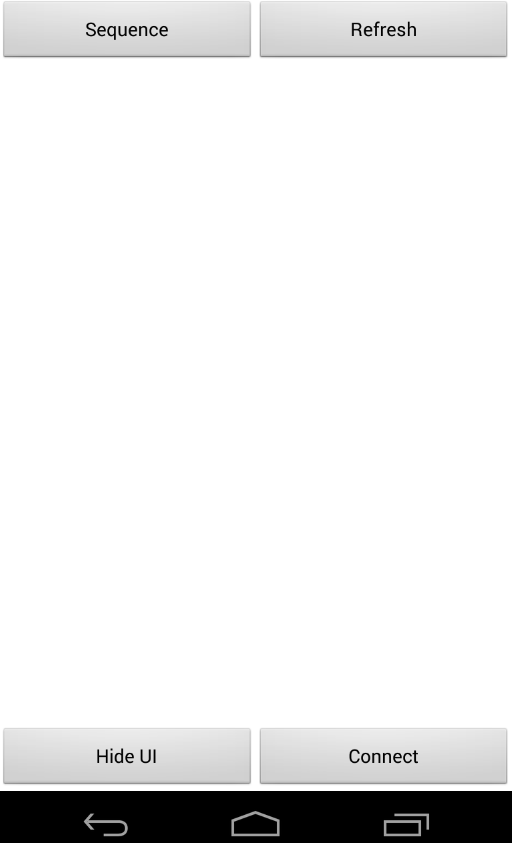
\includegraphics[width=7cm]{conclusion/user_ui.png}
	\caption{Client UI}
	\label{fig:Client_UI }
\end{figure}
\subsection{Functionalities}
\section{Evaluation criteria}
\section{Evaluation Results}
\section{Conclusion}
\section{Discussion}
\section{Further work}
\section{Reflection}
\section{Summary}

\chapter{References}
\input{references/references.tex}

\chapter{Attachments}
\input{attachments/attachments.tex}

\begin{flushleft}
	\bibliographystyle{plain}
	\bibliography{literature.bib}
\end{flushleft}

\appendix
\chapter{User Manual}

\chapter{Installation Guide}

\chapter{Work breakdown structure} \label{txt:work_breakdown_structure}

\begin{figure}[!h]
	\centering
		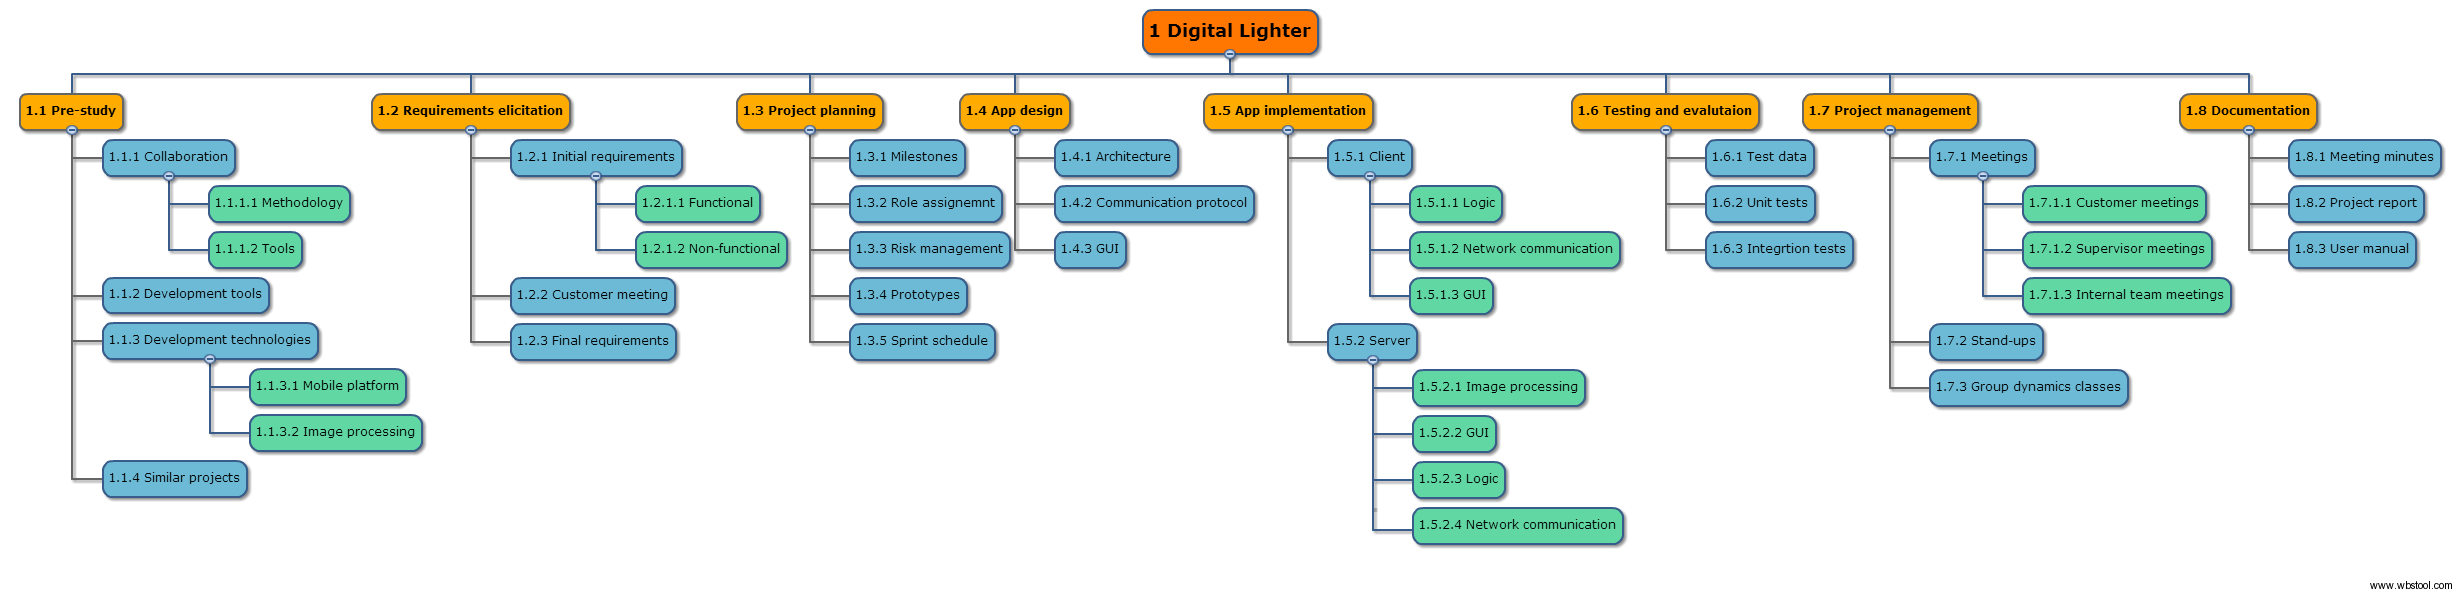
\includegraphics[width=12cm, angle=90]{planning/wbs.png}
	\caption{The work breakdown structure}
	\label{fig:wbs}
\end{figure}

\chapter{Customer meetings}

\chapter{Supervisor meetings}

\chapter{Evaluation Questioner}



\end{document}

%\subsection{Project background}
%\subsection{Source code}
